\chapter{Grammatical domains} \label{chap:3}

This chapter deals with what \citet{Givón1979b} and \citet{HeineEtAl1984} have called the various channels of grammaticalization. The term ``channel'' graphically expresses the fact that the fate of a category in grammaticalization is largely predetermined once we know two things: (1) its meaning, (2) its syntactic function. These conditions are equally necessary. \citet[213f]{Givón1979a} and others have emphasized condition 1, whereas \citet[170]{Meillet1915} had already said: “c'est le rôle dans la phrase qui décide de tout.”

The terms ‘grammaticalization scale’ and ‘grammaticalization channel’ will often be used interchangeably. A \textsc{grammaticalization scale} is a theoretical construct along which functionally similar signs types are ordered according to their degree of grammaticality as measured by certain parameters to be discussed in \sectref{chap:4}. The relation among the elements on such a scale is panchronic. A \textsc{gram\-maticalization channel} is a frequently recurring route which signs with a given function may take when they are grammaticalized in language change. The relation among the elements in such a channel is a diachronic one.

The aim of \sectref{chap:3} is twofold. First, a certain amount of examples of grammaticalization will be accumulated in order to give an idea of the nature of this type of process and to provide suitable empirical material to refer to from the more theoretical chapters to follow. Second, although, naturally, not all parts of the grammar can be treated here, the chapter is meant to demonstrate that grammaticalization is omnipresent and not specific to any particular part of the grammar.

The subdivision of the material follows, in part, from the connections established by grammaticalization channels. But as some channels cross, the presentation will necessarily be somewhat repetitive. The amount of material presented is still greatly reduced in comparison with the masses of evidence available for most of the channels. It would be impossible to display it all here; the reader is referred to the cited literature.

\section{Verbal complexes}

\subsection{Existence and possession}

Verbs such as Engl. \textit{exist}, \textit{possess}, or Latin \textit{existere}, \textit{possidere}, are lexical verbs like any other and have no particular grammatical function. But most languages have more grammaticalized verbs with similar meanings, verbs which roughly correspond to English \textit{be} and \textit{have}.

The various forms of Engl. \textit{be}, as well as of its cognates in other Indo-European languages, go back to three different roots: PIE *\textit{bhew}{}- ‘become’ yields forms such as Engl. \textit{be}, German \textit{bin}, Span. \textit{fuí}\todo{change to fui without accent?}. PIE *\textit{Hes}{}- ‘exist, be in a place’ yields forms such as Engl. \textit{is}, German \textit{ist}, Span. \textit{es}. And Proto-Germanic *\textit{wes}{}- ‘live’ yields forms such as Engl. \textit{was}, German \textit{war}. These are doubtless typical sources of the verb ‘to be’. ‘He lives’ is, for instance, the etymological meaning of the verb \textit{ʔúhki} ‘he is’ in Tunica \citep[41ff]{Haas1941}. Another source of ‘be’-verbs is ‘to stand’. This can be seen in Span./Port. \textit{estar}, French \textit{être}, which derive from Latin \textit{stare}. Among the 15 auxiliaries which \citet[85f]{Žirmunskij1966} cites from Usbek, there are also \textit{quj}{}- ‘stand, place’ and \textit{tur}{}- ‘stand’. ‘To remain’ is the original meaning of the Port. verb \textit{ficar}, which is currently taking over some functions of the verb ‘to be’. These verbs are usually highly irregular or even suppletive, which points to their grammaticalized status.

Engl. \textit{have}, German \textit{haben} and cognates derive from Proto-Germanic *\textit{hafjan} ‘seize’. Span. \textit{tener} ‘have’ meant ‘hold’ in Latin. Anticipating future developments of English, we can say that ‘receive’ is another source: \textit{have} (phonologically /v/ or /z/ or /d/ in the various inflected forms) is currently reinforced by \textit{got} and will soon be entirely renovated by it. These are all, of course, common sources of the possessive verb; see \citet[104-106]{Seiler1983}.

Although there are diachronic derivational relations between ‘be’ and ‘have’ in many languages, there is, interestingly, no unidirectional grammaticalization relation between them. On the one hand, existence predications are often grammaticalized constructions of the verb ‘have’. Thus dialectal German \textit{es hat}, Span. \textit{ha(y)}, French \textit{il y a}, all ‘there is/are’. On the other hand, possessive predications very often contain a verb of existence: Latin \textit{Paulo est liber} ‘Paul has a book’, Mandarin \textit{w\v{o} y\v{o}u yí-zh\=i g\v{o}u} (I \textsc{Exist} one-\textsc{Cl} dog) ‘I have a dog’; cf. also Russian \textit{est'} and Japanese \textit{arimasu}. This is, by the way, an argument against reducing possession to existence or vice versa.

\subsection{The copula} \label{sec:3.1.2}

A copula is a word which turns a nominal into a predicate. This function will not be considered here because it will be treated in subsequent sections. Here we concentrate on the question: through which grammaticalization channels do elements arise which function as the copula in nominal clauses? There are, in principle, two such channels.

As is familiar from Indo-European languages, a copula may be a grammaticalized ‘be’-verb, any one of those treated in the preceding section. In this case, the copula has obviously verbal properties, i.e. it may inflect for person, number, tense etc.; though it may be absent when all the categories are unmarked, as it is, e.g., in Russian.

A less familiar, but equally frequent origin of the copula is a demonstrative or anaphoric pronoun. Consider the case of the Chinese copula, as analyzed by \citet{LiEtAl1977}. In Archaic Chinese, nominal clauses contained no copula. The subject of a nominal predication, especially a relatively heavy one, could be topicalized by left-dislocation. This necessitates a substitute in the subject position of the nominal clause, a demonstrative or personal pronoun which anaphorically takes up the topicalized \np. The resulting nominal clause is, of course, syntactically completely unmarked. The complex sentence structure is as follows: \textsubscript{S}[~\np~\textsubscript{S}[~\textsc{dem} \np~]~]. The \textsc{dem} in Archaic Chinese is \textit{shì}. By the 1. cent. \textsc{ad}, this construction was sufficiently grammaticalized to be reanalyzed as \textsubscript{S}[\np \textsc{dem} \np]. Here \textit{shì} already functions as a copula, one criterion being that it is indifferent as to the person of the subject. About the same time, it ceases to be used as a demonstrative, while in its copula function it becomes increasingly obligatory.

Copulas of this origin may also be found, according to Li and Thompson, in Hebrew, Palestinian Arabic, Wappo and Zway. Such copulas do not, of course, express verbal categories. Since the latter are, in fact, irrelevant to them, they are also not distributed according to marked and unmarked verbal categories, but also appear in what would correspond to a present indicative verbal clause.

The second grammaticalization channel also admits nominal clauses which already contain a copula, which is then reinforced by the pronoun. This is currently happening in French. ‘To live is to learn to die’ is not \textit{Vivre est apprendre à mourir}, but rather \textit{Vivre c'est apprendre à mourir}, which is pronounced, as \citet[72]{Frei1929} insists, “sans pause”.

\subsection{Modals and moods}\label{sec:3.1.3}

Modal verbs or auxiliaries may, of course, derive from full verbs. In what follows, I list some possible sources.

\label{page30}In the Germanic languages, many modal verbs derive from Proto-Indo-\linebreak European \textsc{preterite-presents}, i.e. original full verbs whose inherited perfect form was used with stative present function. Among them are OE \textit{can(n)} ‘know, be able’, \textit{sceal} ‘owe’, \textit{mæg} ‘be able’. These verbs developed a past tense inflection of their own, which made them morphologically highly irregular. Their syntax was still that of common verbs in Old English. During the Middle English period, however, they developed those syntactic pecularities which make them constitute the syntactic category of modal verbs; and as such the verbs \textit{can}, \textit{shall}, \textit{may} and others appear in the 16th century. This development is analyzed in detail by Lightfoot (1979:98ff), though he tries to do without the concept of grammaticalization. A synchronic example for the ambivalence, or transitional status, of a verb between full verb and auxiliary is provided by Romanian \textit{poate} ‘can’; see \citet[198f]{MallinsonEtAl1981}.

\textsc{desiderative} modals such as \textit{will} evolve, of course, from verbs meaning ‘want’. As also shown by English, they may subsequently form the basis of subjunctive auxiliaries such as \textit{would}. The German equivalent is \textit{würde}, but this has a different source. The original meaning of \textit{werden} is ‘become’, and since \textit{würde} is formally subjunctive, its original (still alive) meaning is ‘would become’. In this meaning, the verb formed constructions such as \textsc{ohg} \textit{würde lesende} ‘would become reading’, with a clearly inchoative meaning. The latter, however, disappeared in Middle High German, and in the course of grammaticalization only the subjunctive meaning remained: ‘would read’. Once \textit{würde} had become a sign of the subjunctive, the marked participial form of the verb was no longer necessary. In analogy to the other modal verb periphrases, it was simplified to the infinitive form: \textit{würde lesen}. For this account, see \citet[60f]{Ronneberger-Sibold1980}. The interesting thing about this development is the solution to the problem of reinforcing the subjunctive mood. This was done by extracting this mood from the main verb and using an auxiliary verb as its bearer whose lexical meaning was necessarily irrelevant since its function was nothing more than to carry the subjunctive. This is why, in this construction, it lost its meaning so soon. Contrast this with the formation of the \textit{werden}{}-future dealt with in \sectref{sec:3.1.4}.

The omnipresent existence verb also forms modal constructions, chiefly \textsc{obli\-gative} ones. It combines with nominal verb forms to yield expressions of the type ‘my going exists’, meaning ‘I have to go’. Compare Lat. \textit{mihi est eundum} id., but also Yucatec Maya \textit{yàan in bin} (\textsc{Exist} 1.\textsc{Sg} go) id. Once more, the functional similarity of ‘have’ and ‘be’ in the existence meaning asserts itself here. Thus we have Engl. \textit{I have to go}, and also Vulgar Latin \textit{cantari habet} ‘has to be sung’, which, according to \citet[§~\textsc{ii}]{Benveniste1968}, ultimately yielded the Romance future (cf. below).

Continuing grammaticalization transforms modal verbs into affixes. Examples for the development of desiderative and obligative modals into future markers have already been mentioned and will yet be seen in the following section. The existence of verbal mood affixes is known; besides the common Indo-European subjunctive suffixes, note in particular the Sanskrit desiderative suffix -\textit{sa}. What is lacking in my data is historical evidence for their development out of modal verbs; but on the basis of the analogy to related categories, such evidence must exist.

\subsection{Tense and aspect} \label{sec:3.1.4}

Tense and aspect are often expressed with the help of periphrastic verb constructions in which an auxiliary is used to support a nominal main verb. The two auxiliaries which predominate in Indo-European languages are presumably widespread everywhere: ‘have’ and ‘be’. Both are used in the analytic perfect of the Germanic and Romance languages. For the origin of this construction, see \citet[141-143]{Meillet1912}, \citet[§~\textsc{i}]{Benveniste1968}, \citet{Seiler1973}, \citet{Rosén1980}, \citet{Ramat1983}.\label{page31} In Persian, the auxiliary ‘be’ has been agglutinated to the main verb and now expresses the personal endings of the \textsc{past tense} verb. Similarly, \citet{Haas1977} demonstrates that the personal endings in the conjugation of some Muskogean languages go back to an agglutinated auxiliary.

\citet[130]{HeineEtAl1984} show that in Africa, too, past tenses are frequently expressed with the help of ‘be’. Following \citet[§~5]{Givón1973}, they posit two other possible origins: verbs of motion, especially ‘come’; and verbs meaning ‘to be/have finished’. Both can be exemplified from Portuguese: \textit{vem de escrever} (comes from writing) ‘has written’ (cf. French \textit{vient d'écrire}); \textit{acaba de escrever} (finishes of writing) ‘has just written’. Both of these examples illustrate that past tenses often start out as perfects or perfective aspects; the past meaning actually results from a further grammaticalization. The same is to be observed in the development from the Indo-European perfect to the Germanic past and of the Latin perfect to the Romance simple past tense. And the same is again happening with the ‘passé composé’ in French and the \textit{haben}-perfect in Bavarian German.

%\setcounter{page}{1}
Passing over to \textsc{future tenses}, we again meet ‘have’ here, viz. in Latin-\linebreak Romance. The periphrastic construction ‘infinitive of main verb + form of \textit{habere}’ started in Vulgar Latin, according to \citet[§~\textsc{ii}]{Benveniste1968} in passive clauses, and according to \citet{Ineichen1980} in subordinate clauses. In the course of its expansion, the construction became agglutinative and led to the synthetic Romance future (cf. also \citealt[132--151]{Coseriu1974}). Overall, ‘have’ is probably not so common a future tense auxiliary. Much more wide-spread is ‘go’. It occurs in periphrastic futures in English and various Romance languages, e.g. Port. \textit{vou escrever} (go.1.\textsc{Sg} write:\textsc{Inf}) ‘I will write’. An isolated precedence of this may be seen in the Latin passive infinitive of the future, \textit{scriptum iri} ‘to be going to be written’ (cf. \citealt[109--114]{Ultan1978b}). ‘Go’ also figures in the Usbek and Tunica auxiliary lists given in \citet[85f]{Žirmunskij1966} and \citet[41--51]{Haas1941}, respectively. For African languages, see \citet[§~5]{Givón1973} and \citet[131f]{HeineEtAl1984}.


Since ‘be’ is the counterpart of ‘have’ in so many respects, obligative ‘be’ grammaticalizes to future just as obligative ‘have’ does. An example is provided by Yucatec Maya. The construction \textit{yàan in bin} mentioned in \sectref{sec:3.1.3} is also used colloquially to mean ‘I will go’.

Equally often, the future may arise through the grammaticalization of a desiderative modal. English \textit{will} is a known example. In 13th cent. Greek, an impersonal \textit{thélei} ‘it wishes’ governs a subordinate clause introduced by \textit{ná} ‘that’. This is shortened to \textit{thé ná}, then contracted to \textit{thená} and, by the 16. century, yields \textit{thá} \textsc{Fut}. In Swahili, -\textit{taka} ‘want’ {\textgreater} -\textit{ta}{}- \textsc{Fut}, as illustrated in \REF{ex:E2} (cf. \citealt[131]{HeineEtAl1984}).


\ea\label{ex:E2}
\langinfo{\LangSwah}{}{~\citep[916]{Givón1973}}
 \ea
 \gll n-a-taka ku-la \\   
 \textsc{sbj}.1.\glsg-\textsc{prs}-want  \glinf-eat  \\
\glt ‘I want to eat’
 \ex
 \gll ni-ta-ku-la \\
 \textsc{sbj}.1.\glsg-\textsc{fut}-\glinf-eat\\
 \glt ‘I will eat’ \\
\z
\z
\noindent At a more advanced stage of grammaticalization, we find the Ancient Greek future in -\textit{se/so}{}-, which derives from a PIE desiderative; see \citet[224f]{Rix1976}, and cf. the Sanskrit -\textit{sa}{}-desiderative mentioned in the preceding section.

Finally, future auxiliaries may evolve from verbs with an inchoative meaning. \citet[917]{Givón1973} adduces the example of SiLuyana (Bantu) -\textit{tamba} ‘begin’ {\textgreater} \mbox{\textit{-mba}}-\scfut, as in \textit{ni-mba-kela} (\textsc{sbj}.1.\glsg{}-\scfut-work) ‘I will work’. On the other hand, we have the German future with \textit{werden}. This started at the same time and in the same construction as the \textit{würde}{}-subjunctive mentioned above. Here, again, the original participle of the \textsc{ohg} construction \textit{wird lesende} (‘becomes reading’) is simplified to an infinitive. However, the inchoative meaning here is not discarded, but grammaticalized to a future meaning.

\label{page33}The main source of \textsc{progressive aspect} conjugations is a periphrastic construction formed with the verb ‘be’ plus  a nominalized verb form in some locative dependence. A typical instance of this is the Engl. \textit{she is on working} {\textgreater} \textit{she is a-working} {\textgreater} \textit{she is working}. Compare also the Portuguese variants \textit{está a trabalhar} (stand:3.\glsg at work:\glinf; European) and \textit{está trabalhando} (stand:3.\glsg work:ing, Brazilian). Colloquial German has \textit{ist am arbeiten}, corresponding to the European Portuguese version. One may also be more precise on the nature of the ‘be’-verb involved: Since the construction originally expresses a state (position or condition, ``Befindlichkeit'') of the subject — as is sufficiently proved by the prepositions used —, the verb employed as an auxiliary, if there is a choice, will be the verb ‘be at a place’. It could therefore be predicted that Spanish and Portuguese use \textit{estar} rather than \textit{ser} in their progressive constructions. The same can be seen in African languages. Thus, the Ewe progressive construction \textit{éle vavá \'m} (he:is \rdp:come \glprog) ‘he is coming’ originally expresses a location: \textit{m} derives from *\textit{me} ‘inside’, so that the original meaning is ‘he is in coming’ \citep[105f]{Heine1980}. In Abkhaz \citep[128, 181f]{Hewitt1979}, the postposition \textit{-\k{c}'\`ə} ‘in’ is converted into the intransitive verb ‘be in’ by adding stative verb inflection. The full verb is put into the masdar, an infinitive-like verbal noun, and is constructed as the oblique complement of the auxiliary, as shown in \REF{ex:E3}.

\ea\label{ex:E3} 
\langinfo{\LangAbkh}{}{~\citep[181]{Hewitt1979}}\\
 \gll a-x˚màr-ra  \k{c}\`ə-w+p'\\
{\textsc{art}-play-\glinf}  \textsc{abs}.3-\textsc{obl}.3.\glsg.\textsc{nhum}+in-\textsc{prs}-\textsc{indep}\\
\glt {‘he is playing’}\\
\z
\noindent In Usbek \citep[86]{Žirmunskij1966}, there are four auxiliaries which may be used in the progressive frame ‘main verb-gerund auxiliary-gerund-inflection’, e.g. in \textit{ëz-ib} \textsc{Aux}{}-\textit{ib-man} ‘I am writing’, namely \textit{tur}{}- ‘stand’, \textit{\u{u}t} ‘sit’, \textit{ët }‘lie’ and \textit{jur}{}- ‘walk about’. It is palpable how all these verbs characterize the spatial situation of the subject.\todo{is this layout delibarate?}

\citet[§~5]{Givón1973} and \citet[124-126]{HeineEtAl1984} also point to a second source of progressive aspect markers, namely verbs of the meaning ‘stay’, ‘remain’, ‘keep’. This can also be exemplified from Portuguese, which uses \textit{ficar} (beside \textit{estar}) in progressive constructions.

\label{page33b}For \textsc{habitual aspect/aktionsart}, two sources may be mentioned. The first is a periphrasis with the copula, as for progressive aspect. In Imbabura Quechua, the same suffix \textit{{}-j} which also forms simultaneous relative clauses is used on the full verb. The resulting form is constructed as the predicate complement of the copula. Sentences such as the one in \REF{ex:E4} can nevertheless not be analyzed as containing a syntactically regular free relative clause (see \citealt[149]{Cole1982}).

\ea\label{ex:E4}
\langinfo{\LangQue}{}{~\citep[149]{Cole1982}}\\
\gll Utavalu-pi  trabaja-j  ka-rka-ni\\
Otavalo-\textsc{loc}  work-\textsc{sim}.\textsc{nr}  \textsc{cop}-\textsc{past}-1.\glsg\\
\glt {‘I used to work in Otavalo.’}\\
\z
\noindent Subordinate clauses cannot contain validators (a kind of modal particle). However, in habitual sentences such as \REF{ex:E4}, validators are possible. This shows that there is only one clause in this construction and that non-finite verb plus copula form a periphrastic verb form in it. What started out as a simultaneous nominalizer of clauses ends up as a verb marker of habitual aspect.\label{page34}

The second source of habitual aspect are periphrases which involve the verb ‘do’. Sentences such as \REF{ex:E5} occur in Irish English.

\ea\label{ex:E5} He does plough the field for us. \textup{(John Harris p.c.)}\\
\z
\noindent In Mayan languages, the predicate focus construction is mainly used in order to express habitual aspect, as in \REF{ex:E6} from Yucatec.

\ea\label{ex:E6}
\langinfo{Yucatec}{}{}\\
\gll puroh  káaltal  k-in  bèet-ik\\
 mere  drink  {\textsc{impf}-\textsc{erg}.1.\glsg}  do-\textsc{incompl}\\
\glt {‘mere drinking was what I did’}\\
\z
\noindent Here the full verb becomes non-finite, and the whole predicate is put into focus position. The extrafocal clause reduces to a finite form of \textit{bèet} ‘do’, to which the nominalized predicate is the direct object.

\subsection{Passive and emphasis}\label{sec:3.1.5}

The analytical \textsc{passive} with \textit{esse} ‘be’, which was used, in Latin, only in the perfective categories, replaced the synthetic forms in the Romance languages and yields such passives as Italian \textit{è detto} ‘is said’. This is currently being renovated with the auxiliaries \textit{venire} ‘come’ and \textit{andare} ‘go’. Of these, the unmarked form is \textit{viene detto} ‘is said’; but the contrast with \textit{va detto} evokes the deictic potential of these auxiliaries: the former then implies ‘is said to the speaker’, the latter ‘is said by the speaker’.

The notion of ‘becoming’ is at the basis of the auxiliary which serves in German (\textit{werden}) and Persian (\textit{šodan}) passive constructions; it also appears in the English \textit{get}{}-passive. Because of the basic meaning of the auxiliary, these passives were originally inchoative; \textit{wird grammatikalisiert} would have meant ‘becomes grammaticalized’, the passive meaning being carried exclusively by the participial form of the main verb. With increasing grammaticalization, however, the auxiliary loses its inchoative meaning and becomes a mere carrier of finite verbal categories. This is another example of renovation through complex reinforcement. For other sources of the passive, see \citet[85f]{Givón1979}.

As for \textsc{emphatic constructions}, we will mention here only the auxiliary ‘do’. There are different types of emphatic constructions, and in at least three of them the verb ‘do’ may appear. For the first type, cf. the predicate focus construction mentioned in \sectref{sec:3.1.4}.

Second, the emphasis may not be on a particular sentence constituent, but rather the assertion itself may be emphasized. This type is exemplified in English. According to \citet[55]{Traugott1980}, in Middle English the verb \textit{do} was used as an auxiliary, apart from causative constructions, only if a positive assertion was to be strongly emphasized. By 1700, it came to be used also when the assertion was to be questioned, that is, as an interrogative auxiliary; and by 1900, it appeared also as an auxiliary in negation. The desemanticization accompanying this expansion has led to the situation that \textit{do} is currently being used everywhere with little or no emphasis.

\label{page35}In the third type of emphasis, the main verb is used as a contrastive topic; and due to its being foregrounded, it needs a substitute in the clause. This function is fulfilled by \textit{tun} in Standard German, in sentences such as \textit{Kochen tut sie nicht schlecht} (lit. cooking does she not badly). In Non-Standard German, the auxiliary \textit{tun} has been generalized beyond this context to expressions such as \textit{sie tut nicht schlecht kochen} (cf. p.~\pageref{page123}\chk%102
).

\subsection{Auxiliaries and alternative sources} \label{sec:3.1.6}

The discussion in \sectref{sec:3.1.2}--\sectref{sec:3.1.5} has concentrated on auxiliaries and the like. We will first sum it up and then turn briefly to alternative sources of the grammatical categories mentioned.

The common denominator of the above developments can be characterized as follows: main verb becomes auxiliary verb, possibly via modal verb; this then becomes a mood or aspect marker, and the latter finally a tense marker. The most important and most differentiated instance of this development is certainly represented by the verb ‘be’. It starts out as a ‘verbum substantivum’, a verb of existence. Subsequently, it comes to be used in location predications, with the meaning ‘to be in a place’. Then it appears as the copula in nominal sentences. As such, it may be employed when the predicate is a nominalized verb form, and in this way it ends up as an auxiliary. This development was already posited by \citet[131]{Meillet1912}, who exemplifies it as follows:

\begin{table}
\begin{tabular}{ll}
\lsptoprule
verbum substantivum: & \textit{je suis celui qui }\textbf{\textit{suis}}\\
‘be in a place’: & \textit{je }\textbf{\textit{suis}}\textit{ chez moi}\\
copula: & \textit{je }\textbf{\textit{suis}}\textit{ malade}\\
auxiliary: & \textit{je }\textbf{\textit{suis}}\textit{ parti}\\
\lspbottomrule
\end{tabular}
\end{table}

As was already mentioned with reference to Persian and Muskogean, further grammaticalization yields inflectional endings.

The grammaticalization of full verbs to auxiliaries shows us two things. First, a piece of methodology: The dispute on whether auxiliaries are main verbs or not (J. Ross: yes; L. Palmer: no; R. Huddleston: yes; etc.) is fruitless. Two grammatical categories connected on a grammaticalization scale are neither the same nor distinct. The difference between them is gradual, and there is no clear-cut dividing line. Secondly, an empirical insight: Grammaticalization can turn syntactic relations around. In a word combination which contains two verb forms, one of which will become the auxiliary in an analytic construction, this latter one starts by being the syntactic (not lexical!) main verb (cf. \citealt[96f]{Givón1979}), while the other, governed verb carries the major part of the lexical meaning.\footnote{The term 'main verb' is, unfortunately, ambiguous. In its syntactic sense, it means the governing verb; and in this sense the auxiliary in an analytic verb phrase is the main verb, as is argued above. In its semantic sense, it means, within an analytic verb form, that verb which carries the lexical meaning, and consequently denotes the exact opposite of the first sense. The term denoting the second sense should probably be ``full verb''.} However, only a free form can exert government. As, in the course of proceeding grammaticalization, the auxiliary loses its verbal properties, it can no longer be said to govern the lexical verb.\label{page36} When it has become a tense/mood/aspect marker, it depends on the lexical verb, which is now the main verb. Thus, the syntactic relations are almost reversed; though not quite, because within a word there are no syntactic, but morphological relations. We shall find (\sectref{sec:4.3.2}) that this development of relations is characteristic of grammaticalization processes. For the trouble that intermediate stages of this development may cause to synchronic analysis, see \citealt[155f]{Matthews1981}.

\newpage
We now turn to alternative sources of the verbal categories treated above. There appear to be two principal ones: serial verbs and adverbs. Serial verbs will be treated in more detail in \sectref{sec:3.4.1.7}, as a source of adpositions. They have, in fact, been studied mainly in that connection, and comparably little attention has been devoted to their aspectual or aktionsart function.

\label{page37}I cannot clarify here the complex and much debated issue of the syntactic relations among the verbs in a series. Let us assume the following definition: a \textsc{serial verb construction} is the combination of two or more asyndetically juxtaposed verbs with at least one shared argument in order to express a complex, but unitary situation. In the course of grammaticalization of a serial verb construction, one verb in a pair undergoes the usual symptoms of grammaticalization, becoming, in the last event, a grammatical formative, while the other remains virtually unaffected.\footnote{An alternative development is that a pair of verbs in a series becomes a compound verb; but this is not grammaticalization; see §~5.2.} I shall refer to that member of a series which is (destined to be) grammaticalized as ‘the \textsc{serial verb}’ in the construction. This terminology is based on the assumption that wherever verb serialization occurs, there is a relatively closed class of verbs with an active serialization potential (the serial verbs), combining with verbs from an open class which are indifferent to serialization. Such serial verbs which develop into adpositions are called ``coverbs'' in the literature and will be dealt with in \sectref{sec:3.4.1.7}.

Examples of serial verbs with aspectual function may be adduced from Niger-Congo languages (see also \citealt[113--117]{Sasse1977a} on Mba). In Akan (Kwa), there is a verb \textit{bá} ‘come’ which has developed a grammatical function as the first verb in a series \citep[353f]{Welmers1973}. In this position, it has become a future marker, which is subject to phonologically conditioned allomorphy and has become prefixed, together with its personal prefix, to the following full verb. This is the origin of such forms as \textit{\'ɔ-bέ-bá} (3.\textsc{sg-fut}-come) ‘he's going to come’ or \textit{ò-bé-dìdí} (3.\textsc{sg-fut}-eat) ‘he's going to eat’. In Efik (Benue-Kongo), the verb \textit{mà} ‘fulfill, accomplish’ takes the first position in a series. Here it is grammaticalized to a neutral past marker and undergoes tonal assimilation, as in the following examples \citep[371]{Welmers1973}: \textit{ì-mà í'dí} (we-\past we-come) ‘we came’; \textit{\'m'má ń-dí} (I-\past I-come) ‘I came’.

%\setcounter{page}{1}
More evidence for serial verbs in aspectual function comes from Creole languages. Tok Pisin (New Guinea) provides us with the following examples (from \citealt{Mosel1980}):

\xbox{\textwidth}{
\ea\label{ex:E7}
\langinfo{\LangTok}{}{~\citep[108]{Mosel1980}} \\
\gll ol  manmeri  bilong  Papua  Niu  Gini  i  save  kaikai  kaukau\\
\textsc{pl}  man  of  Papua  New  Guinea  \textsc{sbj}.3  \textsc{hab}  eat  {sweet potato}\\
\glt ‘Papua New Guineans eat sweet potatoes.’\\
\z
}
\noindent Portuguese provided the verb \textit{saber} ‘know, can’, which has become \textit{save} ‘to do habitually’ in Tok Pisin. This enters verbal series as the first member and ends up as an aspectual marker, as in \REF{ex:E7}.

English \textit{stop} yields \textit{stap} ‘live, be located’ in Tok Pisin. This enters a verbal series as the last member and develops into a marker of continuous action, as in \REF{ex:E8}.

\ea\label{ex:E8}
\langinfo{\LangTok}{}{~\citep[108]{Mosel1980}}\\
\gll em  i  wok  i  stap  yet\\
 he  \textsc{sbj}.3  work  \textsc{sbj}.3  \textsc{cont}  self\\
\glt {‘he is/was still working’}\\
\z
\noindent A similar fate has befallen English \textit{finish}; this has become a postverbal completive aspect marker in Tok Pisin:

\ea\label{ex:}
\langinfo{\LangTok}{}{~\citep[123]{Mosel1980}} \\
\gll em  i  go  pinis\\
he  \textsc{sbj}.3  go  \textsc{compl}\\
\glt {‘he has/had/will have gone’}\\
\z
\noindent I shall gloss over several problems in these examples. It is evident, for instance, that in some of them the serial and the full verb each have their own personal prefixes, whereas in others only one of them has. Furthermore, the question naturally arises as to whether we need to treat grammaticalized serial verbs as distinct from auxiliaries or modal verbs. All the examples seem to be interpretable in either of these two terms. This would mean that we have only found a new source of auxiliary verbs, but not a new source of mood/aspect/tense markers, since these would still derive from auxiliaries. Much seems to speak in favour of this position. On the other hand, the morphological difference just mentioned might correlate with a difference among serial, modal, and auxiliary verbs. The latter distinction might also account for the positional differences in the last three examples. \citet[128]{HeineEtAl1984} have an intriguing example from Ewe (Kwa). The language has serial verb constructions in which the serial verb follows the full verb(s). It also has auxiliaries which precede full verbs. There is a verb \textit{nɔ} ‘remain, stay’ which has been grammaticalized to a habitual aspect marker. In standard Ewe, this is constructed as a serial verb, e.g. \textit{me-yí-na} (I-go-\textsc{Hab}) ‘I am in the habit of going’. In the Dahome dialect of Ewe, however, \textit{nɔ} is constructed as an auxiliary, as in \textit{m-nɔ-sa} (I-\textsc{Hab}{}-sell) ‘I am in the habit of selling’.

Faced with problems such as this, I prefer to take no stand on the issue of whether (some of) the grammaticalized serial verbs in the above examples are to be analyzed as auxiliary or modal verbs. It suffices to say that these categories are functionally and structurally quite similar.

We finally turn to a definitely different source of tense markers. \citet[218f]{Givón1979a} raises the question whether tense/mood/aspect distinctions can arise from \textsc{adverbs}, and answers it in the negative. Available evidence, however, argues for a more differentiated hypothesis: while modal and aspect markers appear, in fact, to derive exclusively from periphrastic verbal constructions, tenses may come from adverbs (see also \citealt[Ch. 3.1.1.3]{HeineEtAl1984}). There are probably quite a number of languages which use a word meaning ‘already’ in the function of a past or perfect tense marker; Indonesian \textit{sudah} is one example. Future markers deriving from adverbs can be exemplified from creole languages \citep{Labov1971}. English \textit{by and by} has yielded the free future temporal adverb \textit{baimbai} of the pidgin stage of Tok Pisin (which lacks tense). This was subsequently simplified and grammaticalized to a preverbal future marker, which may cooccur with future adverbs, as in \textit{klostu bai i dai} (soon \textsc{Fut} \textsc{Sbj}.3 die) ‘he'll die soon’. In the present creole language, it has become increasingly obligatory and is further phonologically reduced to \textit{be} (cf. also \citealt{SankoffEtAl1974}). Spanish \textit{luego} ‘soon’ underwent a maximally parallel fate in Papiamento: it was reduced to \textit{lo} and became a preverbal future marker, as in \textit{lo mi kanta} (\textsc{Fut} I sing) ‘I will sing’.\label{page39b} Adverbs which are grammaticalized to future and past tense markers and adjust their position vis-à-vis the verb accordingly have also been found in the Nilotic languages Luo, Lotuko and Bari \citep[130, 132]{HeineEtAl1984}.\label{page39} Finally, according to an Indo-Europeanist hypothesis of long standing, the final \textit{{}-i} common to the so-called primary verbal desinences is an original deictic particle. While a reconstruction, obviously, does not count as evidence, the other cases clearly show that the development ‘adverb → tense marker’ must be posited as a grammaticalization channel.

The developments discussed in the preceding sections may be summarized in \figref{fig:interrelated}.

%\setcounter{page}{1}

 
%%please move the includegraphics inside the {figure} environment
%%\includegraphics[width=\textwidth]{\textsc{thoughts}-img1.svm}
 
%%please move the includegraphics inside the {figure} environment
%%\includegraphics[width=\textwidth]{\textsc{thoughts}-img2.svm}
 
%%please move the includegraphics inside the {figure} environment
%%\includegraphics[width=\textwidth]{\textsc{thoughts}-img3.svm}

%\begin{tabular}{llllll} 
%\lsptoprule
%   & modal verb &  &  & mood marker & \\
%full verb &  &  & auxiliary verb &  & \\
%&  & serial verb &  & aspect marker & \\
%adverb &  &  &  &  &  tense   marker\\
%\lspbottomrule
%\end{tabular}

\begin{figure}

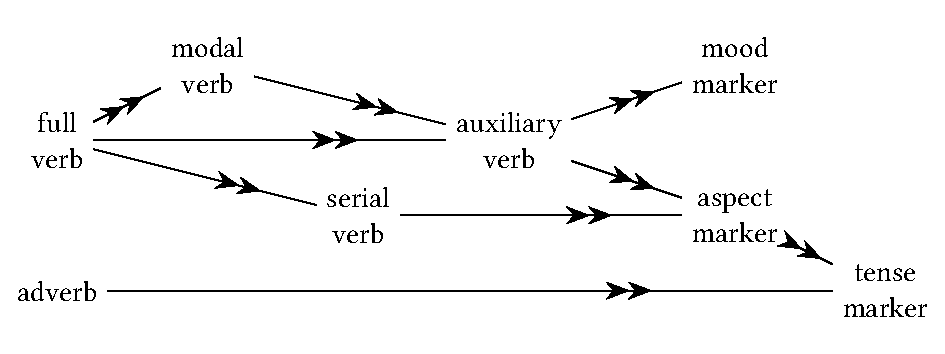
\includegraphics[width=.9\textwidth]{figures/2-someintverbcat.pdf}
\caption{Some interrelated grammaticalization channels of verbal categories}\label{fig:interrelated}
\end{figure}


\section{Pronominal elements}\label{sec:3.2}

I shall not deal here with all the different kinds of pronouns. A major distinction will be made between definite and indefinite pronominal elements. Under the category of definite pronominal elements I will treat demonstratives, definite articles and personal pronouns, as well as their products in grammaticalization. The heading of indefinite pronominal elements will comprise indefinites properly speaking, indefinite articles and interrogative pronouns, and again their grammaticalization products.

\subsection{Definite pronominal elements}

There is one type of pronoun at the root of this family, and this is the free \textsc{demonstrative pronoun}. In its full, ideal form, this contains three components, two semantic and one syntactic. First, the demonstrative element in the narrow sense, which embodies definiteness and a pointing gesture. Second, what we may call the deictic element, which directs the attention to something located in regard to the speech situation (speaker vs. hearer, visible vs. invisible, etc.). Third, a categorial element, either \np or \gldet, which renders the pronoun either syntactically autonomous or dependent. Of these, the deictic component will usually be segmentally expressed at the stage of the free demonstrative pronoun (otherwise it fuses with the demonstrative one). Either the demonstrative or the categorial component will almost always lack expression. The Yucatec Mayan discontinuous (or circumfixal) demonstratives express the demonstrative and the deictic components separately. We have the following paradigm:

\begin{table}[H] % maybe instead of H we should insert some reference into the text
\begin{tabular}{ll}
\lsptoprule
\textit{le} \np-\textit{a'} & ‘this \np’\\
\textit{le} \np-\textit{o'} & ‘that \np’\\
\textit{le} \np-\textit{e'} & ‘aforementioned \np’\\
\lspbottomrule
\end{tabular}
\end{table}

The Japanese demonstrative (and other) pronouns express the deictic and the categorial components separately, as shown in the following paradigm:

\begin{table}[H] % maybe instead of H we should insert some reference into the text
\begin{tabular}{llll}
\lsptoprule
\multicolumn{2}{l}{\textsc{pronoun}} & \multicolumn{2}{l}{\textsc{proadjective}}\\
\itshape ko-re & ‘this one’ & \textit{ko-no} N & ‘this N’\\
\itshape so-re & ‘that one’ & \textit{so-no} N & ‘that N’\\
\itshape a-re & ‘yonder one’ & \textit{a-no} N & ‘yonder N’\\
\lspbottomrule
\end{tabular}
\end{table}

The first step in the grammaticalization of the demonstrative pronouns is the weakening of the deictic component. Deictic distinctions tend to be neutralized, the paradigm is reduced, and at the same time its unmarked member, namely that of third person deixis, assumes a primarily anaphoric function. An example, Latin \textit{ille}, has already been mentioned in \sectref{sec:2.2}. A case of extreme reduction is provided by Vulgar Latin *\textit{ecce hoc ill\=ac} ‘lo this over there’{\textgreater} French \textit{cela} ‘that’ {\textgreater} \textit{ça} ‘it’. We disregard for the moment the fate of the more marked demonstrative pronouns (see §~6.3) and concentrate on the further development of the unmarked one. There are two principal grammaticalization channels, corresponding to whether the categorial component is \np or \textsc{det}; and we will subdivide the discussion accordingly.

\subsubsection{Definite determiners}
At the present stage of the development, we have an adnominal demonstrative pronoun which is deictically neutral and therefore mainly used for anaphoric purposes. Examples, besides Late Latin \textit{ille}, are Gothic \textit{sa}, \textit{s\=o}, \textit{Þata}, OE \textit{s\=e}, \textit{s\=eo}, \textit{thæt} and Homeric \textit{hó}, \textit{h\'{\=e}}, \textit{to}, all deriving from PIE *\textit{so}, \textit{s\=a}, \textit{tod}. Persian \textit{\=an} and Japanese \textit{sono} appear to be well on their way towards this stage.

The following development has been described by \citet{Greenberg1978} for African languages (cf. also \citealt[§~3]{Givón1978}), but it occurs in languages all over the world. The demonstrative component is gradually reduced to mere definiteness, and the result is a \textsc{definite article}. We thus get French \textit{le}, \textit{la}, \textsc{ohg} \textit{ther}, \textit{thiu}, \textit{thaz}, Engl. \textit{the} and Attic \textit{ho}, \textit{h\=e}, \textit{to}. Further grammaticalization agglutinates the article to the noun. Suffixed articles occur in Romanian, Swedish, Danish, Basque, Ijo (Kwa), Koyo (Kru) and Yuman languages such as Mohave, Diegueño and Yavapai. Prefixed articles occur in Abkhaz (Caucasian) and Arabic vernaculars.\label{page42} The Swedish case illustrates that while the definite article is typically in opposition to a demonstrative, a definite affix starts cooccurring with other definite elements.

At this stage, further semantic weakening leads to a reduction of definiteness to specificity. This is largely true for the Abkhaz article and for the suffixed article of Dagbani (Gur). If this last bit of referential meaning is lost, too, we are left with the categorial component of the erstwhile demonstrative. That is, the element then signals only that the word it is attached to is a noun, and can therefore still be used as a nominalizer (which is an important function of the definite article, anyway). See \citealt[§~3.5]{Greenberg1978} on the nominalizing -\textit{s} of Plateau Penutian.\label{PlateauPenutian}

If the demonstrative pronoun which is at the beginning of this process expresses any noun class or gender distinctions — the primary locus of which is, in fact, the pronoun —, then these will go all the way along, and when the specificity of the article is lost, they will be left as \textsc{noun class markers}. This appears to be a plausible account of the genesis of nominal gender or class markers as they occur, for instance, in Bantu languages (details in \citealt[§~7.2]{Lehmann1982b}).

\subsubsection{Personal pronouns} \label{sec:3.2.1.2}
We go back again to the stage of Early Latin \textit{is}, Late Latin \textit{ille}, Gothic \textit{sa}, Homeric \textit{hó} and Bambara \textit{ò}. One thing that often happens to such anaphoric pronouns with a slight demonstrative force is that they come to be used as relative pronouns. This happened, for instance, to \textsc{ohg} \textit{ther} and to Homeric \textit{hó}. The development is treated in detail in \citet[Ch.~\textsc{vi}.1.1.2 and 1.2.2]{Lehmann1984}. Although this is a deviation from the main channel, it certainly is a grammaticalization, since the pronoun loses its demonstrative force and definiteness (cf. \citealt[Ch. \textsc{v}.2.3, §2]{Lehmann1984}) and becomes syntactically obligatory in a certain construction.

Returning to the main thread, we find the pronouns here losing their demonstrative force, too. The result is a \textsc{free personal pronoun} as exemplified by Proto-Romance *\textit{illu}, Engl. \textit{he} or German \textit{er}. The latter two derive, in fact, from the PIE demonstrative *\textit{ei-s} which also yielded Latin \textit{is}. Having thus arrived at a third person pronoun, let us now turn to first and second person pronouns and discuss briefly their possible origin.

New pronouns, especially for the second person singular, are often obtained by shifting pronouns around in the paradigm, especially by substituting marked forms for unmarked ones. This explains, e.g., the use of German \textit{Sie}, French \textit{vous} and English \textit{you} for the second person singular (see \citealt[112]{Syromjatnikov1980} for Japanese). Again, a new first person plural pronoun is being formed in French and Portuguese by what has so far been the non-specific indefinite pronoun ‘one’, namely \textit{on} and \textit{a gente}, respectively. Here grammaticalization plays no part.

However, new forms may also come from outside the paradigm; nouns may be grammaticalized to pronouns. In Spanish, \textit{vuestra merced} ‘your grace’ has yielded the honorific second person pronoun \textit{usted}, whose plural \textit{ustedes} has already ousted, in South America, the original plain form \textit{vos(otros)}. The Portuguese product of \textit{vossa mercê}, \textit{você}, is used in most parts of Brasil instead of the original \textit{tu}.\footnote{In Rio de Janeiro, even dogs are addressed by \textit{você}.} Japanese provides the following examples: \textit{watakusi} lit. ‘my private affair’ {\textgreater} \textit{watasi} ‘I’ (hon.); \textit{boku} (Chinese loan) ‘slave’ {\textgreater} ‘I’; Old Jap. \textit{kimi} ‘lord’ {\textgreater} ‘you’ (hon.) {\textgreater} ‘thou’; \textit{anata} lit. ‘that part’ {\textgreater} ‘you’ (hon.); \textit{omae} (\textsc{Hon}:front) {\textgreater} ‘thou’ (vulg.) (from \citealt{Syromjatnikov1980} and Yoshiko Ono, p.c.). Vietnamese \textit{tôi} ‘I’ comes from a word meaning ‘subject’ (Wilfried Kuhn, p.c.). The Indonesian \textit{saya} ‘I’ derives from a literate word \textit{sahaya} ‘servant’ (which in turn comes from Sanskrit \textit{sah\=aya} ‘assistant’); and \textit{tuan} ‘you’ (hon.) is an original Arabic loan meaning ‘master’ \citep[152]{Gabelentz1891}. In East-Asia, the use of relational nouns instead of personal pronouns whenever there is a personal relation between the discourse participants is wide-spread and liable to yield rich material for the grammaticalization origin of first and second person pronouns.

\label{page43}We see that personal pronouns derive from two entirely different sources: whereas those of the third person come from demonstratives, those of the first and second persons come from nouns of social relations. There is no a priori reason why the grammaticalization processes which lead to these two kinds of personal pronouns should take a parallel course. It is therefore no wonder that we find many languages where the third person pronouns are not well integrated into the paradigm. Several of the ancient Indo-European languages are examples of this, as their third person pronouns retain a slight demonstrative force which is, of course, absent from the first and second person pronouns. And there are quite a number of languages which are conventionally said to lack third person pronouns altogether, a situation which we might rephrase by saying that what would be the third person pronouns are either too little or too much grammaticalized to be able to fulfill that function. Such languages are Walbiri, Dyirbal, Mangarayi (North Australia; \citealt[99]{Merlan1982}), Japanese, Lakhota (Sioux) and Basque. This situation repeats itself in the personal affixes of many languages: there are paradigms in which the third person (singular) affix is zero (although this may also be explained by its semantic unmarkedness). On the other hand, the genetic and functional difference of the two kinds of pronouns does not necessarily prevent them from forming an integrated paradigm and behaving maximally similar, as they do, for instance, in English, German, Russian, Arabic, Turkish and Chinese. Such paradigmatic differences will be disregarded in what follows. For more details on the subsequent development, see \citealt[§§~6.2 and 7.1]{Lehmann1982b}.

When personal pronouns are deaccentuated, they become clitic, usually either in Wackernagel's position or to the word which governs them. Examples are the oblique pronouns \textit{le}, \textit{la} etc. in Italian, French and Spanish or the forms \textit{ne}, \textit{se}, \textit{s} of Northern Substandard %
%Politisch korrekt ist 'Nonstandard'.
German (e.g. \textit{Ich habe ne/se/s doch gestern gesehen}! ‘But I saw him/her/it yesterday!’). Such forms are frequently phonologically reduced in comparison with eventually coexisting stressed forms.\label{page44b} While full personal pronouns may have the same distribution as lexically headed \nps, \textsc{clitic pronouns} are often confined to certain positions. Many languages, such as Modern Greek and Romance languages, have a set of primary prepositions which require a full \np or personal pronoun as their complement and do not accept a clitic pronoun.

Clitic pronouns become fillers of syntactic positions which may not be left open. In Italian, for instance, if the direct object is topicalized by left-dislocation, it must be represented in the clause by a clitic pronoun, as in \textit{Giovanni}, \textit{l'ho visto ieri}. ‘John, I saw (him) yesterday.’ (cf. \citealt[154]{MallinsonEtAl1981}). In Spanish, the clitic object pronoun may even cooccur with a nominal object within a clause, as in \textit{Ayer lo vi a Juan}. ‘Yesterday I saw John.’\label{page44} At this stage, the pronoun potentially loses its anaphoric function and becomes an \textsc{agreement marker}. At about the same time, it turns from a clitic into an affix (cf. \citealt[496f]{Humboldt1836} on this phase of the development). In this way, the carrier of the affix acquires the morphological categories of person, number and gender/noun class.\footnote{On p.~\pageref{page31}\chkfn%25
it was mentioned that a verb may acquire such categories through the agglutination of an auxiliary which possesses them. Ultimately, however, this is probably not an alternative, since the auxiliary, in turn, must have acquired these categories somehow.} Simplifying somewhat, we call these \textsc{personal affixes}. They may appear on verbs (for subject, direct and indirect object), nouns (for the possessor) and adpositions (for the complement). There are a number of languages such as Navaho, Abkhaz or Arosi, which have all three of these types. \REF{ex:E10} contains examples from Abkhaz \citep[105, 116, 103]{Hewitt1979}. \enlargethispage{2\baselineskip}

\ea\label{ex:E10}
\langinfo{\LangAbkh}{}{} \\
 \ea
 \gll (sarà)  a-x°əč'-k°à                  a-š°q°'-k°à                          Ø- r\'ә- s- to -yt'.\\
I            \textsc{art}-child-\textsc{pl}  \textsc{art}-book-\textsc{pl}  \textsc{abs}.3.\textsc{pl}- \textsc{io}.3.\textsc{pl}.\textsc{hum}- \textsc{erg}.1.\glsg- give.\textsc{dyn} -\textsc{indep}\\
\glt ‘I give the books to the children’
\ex 
\gll à-č'k°'ən  yə-y°nr\'ә\\
 \textsc{art}-boy  \textsc{obl}.3.\textsc{sg.m}-house\\
\glt ‘the boy's house’\\
\ex
\gll a-yr\'әyas  a-q'+nr\'ә\\
 \textsc{art}-river  \textsc{obl}.3.\glsg.\textsc{nhum}-at\\
\glt ‘at the river’\\
\z
\z
\noindent In the cases cited, the personal agreement affixes may still function (anaphorically) as personal pronouns, when no \np is present in the same construction. Further semantic weakening makes them lose this ability, and they become entirely conditioned by agreement. The personal endings of the finite verb in French, Russian and German illustrate this stage of the development. If grammaticalization proceeds further, the personal agreement affixes become invariable markers. The subject affixes of the verb become elements which identify the category ``verb'' or the constituent ``predicate'', and its object affixes become transitivity markers. Both these developments have occurred to the erstwhile pronouns \textit{he} and \textit{him}, respectively, in Tok Pisin. The resulting invariable morphemes, the preverbal \textit{i}{}- and the postverbal -\textit{im}, are exemplified in \REF{ex:E11}.

\ea\label{ex:E11}
\langinfo{\LangTok}{}{~\citep[67f]{Sankoff1977}} \\
\gll  Man  i-mek-im  singsing\\
man  \textsc{sbj}.3-make-\textsc{tr}  spell\\
\glt {‘Men utter a spell’} \\
\z
\noindent This is the final stage in the grammaticalization of personal pronouns before their disappearance.

\subsubsection{Reflexive pronouns} \label{sec:3.2.1.3}
The grammaticalization of reflexive pronouns has been studied recently by \citet[esp. Ch. \textsc{iv}]{Faltz1977}, \citet[640--647; largely based on Faltz]{Edmondson1978} and \citet{Strunk1980}. Several of my examples are drawn from these sources, and the following discussion, too, is indebted to them. Just as it would be difficult to formulate a common grammatical denominator for all the different phenomena arranged on a grammaticalization scale together with personal pronouns and treated in the preceding section, so it is difficult to find a single grammatical denominator for all the phenomena which are commonly called reflexive and which we will again find to be arranged on a grammaticalization scale. Their common denominator lies precisely in the fact that they are connected by a grammaticalization channel, this in turn being determined by a function which might be roughly characterized as marking identity with or back reference to an entity involved in the same proposition (sentence or clause); cf. \citealt{Plank1979a}.

I will simplify the discussion a bit by assuming the following four categories, enumerated here in the order of increasing grammaticalization:

\begin{enumerate}
 \item[(i)]   autophoric nouns, e.g. Sanskrit \textit{\=atmán} ‘soul’;
 \item[(ii)]  reflexive nouns, e.g. English \textit{self};
 \item[(iii)]  reflexive pronouns, e.g. German \textit{sich} ‘oneself’; 
 \item[(iv)]  verbal reflexives, e.g. Russian -\textit{sja}.              
\end{enumerate}


\noindent It does not need to be emphasized that the boundaries between these categories are fluid.

There is a whole set of notions centering around the person, as a whole or in part, which are generalized in many languages to comprise the self and which I call \textsc{autophoric}. Typical examples are Sanskrit \textit{tan} ‘body, person’ and \textit{\=atmán} ‘breath, soul’, Buginese \textit{elena} ‘body’, Okinawan \textit{d\=una} ‘body’, !Xu \textit{l'esi} ‘body’, Basque \textit{burua} ‘head’, Abkhaz \textit{a-x} ‘the head’. In their respective languages, all these nouns are translation equivalents of English \textit{self}. As relational nouns, they are often accompanied by a (reflexive) possessive pronoun. Typical examples from Vedic \citep[207f]{Delbrück1888} are:

\ea\label{ex:12}
\langinfo{\LangVed}{}{~\textsc{rv} 7,86,2}\\
\gll utá  sváy\=a  tanv\`{\=a}  sám  vade  tát\\
 and  \textsc{poss}.\textsc{refl}:\textsc{inst}.\glsg.\textsc{f}  self:\textsc{inst}. \glsg.\textsc{f}  together  speak:I  that:\textsc{acc}.\glsg.\textsc{n}\\
\glt {‘and I converse thus with myself’}\\
\z
\noindent \ea\label{ex:13}
\langinfo{\LangVed}{}{~\textsc{rv} 9,113,1} \\
\gll bálam  dádh\=ana  \=atmáni\\
strength:\textsc{acc}.\glsg.\textsc{m}  put:\textsc{part}.\textsc{pf}.\textsc{mid}  self:\textsc{loc}.\glsg\\
\glt {‘putting strength in myself’}\\
\z
\noindent At the other end of the spectrum, Old Indic makes use of a middle voice, which will be discussed below.

The difference between an autophoric and a \textsc{reflexive noun} in the present conception is mainly one of transparency or etymologizability. That is, autophoric nouns are ordinary nouns with free non-reflexive uses; reflexive nouns are nouns meaning ‘self’ and nothing else. Examples are German \textit{selbst}, Latin \textit{ipse}, Spanish \textit{mismo}, Italian \textit{stesso}, Finnish \textit{itse}, Hungarian \textit{magan}, Turkish \textit{kendi}, Japanese \textit{zibun} and Yucatec \textit{báah}. Some illustrative sentences are:

\ea\label{ex:E14}
\langinfo{\LangGerm}{}{}\\
 \ea
 Ich komme selbst.\\
  
\glt ‘I am coming myself.’\\
\ex 
\glt Wollen Sie die Karten für sich selbst?  (cf. \REF{ex:E15})\\
\z
\z
\noindent \ea\label{ex:E15}
\langinfo{\LangFinn}{}{}\\
\gll Halu-at-ko  lipu-t  itse-lle-si?\\
 want-2.\glsg-\textsc{int}  ticket-\textsc{acc}.\textsc{pl}  self-\textsc{all}-\textsc{poss}.2.\glsg\\
\glt {‘Do you want the tickets for yourself?’}\\
\z
\noindent 
Reflexive nouns are a heterogeneous class. In some languages, for instance Finnish, Hungarian, Turkish and Yucatec, they take possessive affixes, just like autophoric nouns (cf. Engl. \textit{myself}, \textit{yourself}). In others, such as German or the Romance languages, they are not normally combined with possessive pronouns. Again, in some languages such as Japanese and Yucatec, a reflexive noun can by itself function as a reflexive pronoun; in others such as German, Latin and the Romance languages, a reflexive noun can only accompany appositively a reflexive pronoun or another noun in order to emphasize the identity. Reflexive nouns of the latter subtype are formally similar or identical to the (pro-)noun of identity, ‘same’; this is so with German \textit{selb-}, Italian \textit{stesso}, Spanish \textit{mismo}. They are somewhat marginal to the grammaticalization channel; but they may enter it if used in reinforcement; see below.

\textsc{reflexive pronouns} function syntactically like ordinary personal pronouns. Examples are German \textit{sich}, Russian \textit{sebja}, Latin-Romance \textit{se}, \textit{si}, \textit{soi}. Because of their primary function to refer back to the subject, reflexive pronouns normally lack a nominative. Instead, an appositive reflexive noun will normally appear, as in \REF{ex:E14}.a above. Just as ordinary personal pronouns have reflexive counterparts, so ordinary possessive pronouns may have reflexive counterparts. Examples are Latin \textit{suus} (as opposed to \textit{eius}), Portuguese \textit{seu} (as opposed to \textit{dele}) and Russian \textit{svoj} (as opposed to \textit{ego}). As these examples show, the proper possessive pronouns may be inherently reflexive, while the non-reflexive forms are in fact genitives of the personal pronouns.

\textsc{verbal reflexives} are verb affixes expressing that the action somehow affects the subject. Examples are:

\ea\label{ex:E16}
\langinfo{\LangTurk}{}{~\citep[156]{Wendt1972}}\\
\gll Çocuk  yıka-n-dı.\\
 child  wash-\textsc{refl}-\textsc{past}\\
\glt {‘The child washed himself.’}\\
\z
\noindent \ea\label{ex:E17}
\langinfo{\LangMang}{}{~\citep[135]{Merlan1982}} \\
\gll jalŋa  Ø-bu-yi-ni  a-andi\\
hard  3.\glsg-hit-\textsc{refl}-\textsc{past}  \textsc{n}.\textsc{inst}-stick\\
\glt {‘He hit himself hard with a stick.’ }\\
\z
\noindent \ea\label{ex:E18}
\langinfo{Greek}{}{~(Pl. \textit{Gor.} 7, 452)}\\
\gll   khr\=ematists  hoûtos áll\=oi  anaphansetai  khr\=ematizómenos\\
 businessman:\textsc{nom}.\glsg.\textsc{m}  \textsc{d}\oldstylenums{1}:\textsc{nom}.\glsg.\textsc{m}  other:\textsc{dat}.\glsg.\textsc{m} {show:\textsc{fut}:\textsc{mid}.3.\glsg} trade:\textsc{part}.\textsc{prs}.\textsc{mid}:\textsc{nom}.\glsg.\textsc{m}\\
\glt {‘this businessman will appear to acquire for somebody else’}\\
\z
\noindent The verb forms in \REF{ex:E16}--\REF{ex:E18} are opposed to unmarked active verb forms: thus compare \textit{yıka-dı} ‘he washed’ with \REF{ex:E16}, \textit{bu-ni} ‘he hit’ with \REF{ex:E17} and \textit{anaphansei} ‘he will show’ and \textit{khr\=ematíz\=on} ‘trading’ with \REF{ex:E18}. Following traditional terminology, I have dubbed the affixes in Turkish and Mangarayi ``reflexive'', but the Greek affix ‘middle (voice)’. There is, in fact, a structural difference in that the reflexive affixes here come near the verbal stem and are almost derivational, whereas the morphological category of middle in Greek is amalgamated with the personal desinences. On the other hand, the Turkish and Greek categories have in common that both are largely ambiguous between reflexive and passive, while the Mangarayi category is ambiguous between reflexive and reciprocal. In all three languages, the reflexive fills the position of a voice or valence-changing verbal derivation. Reflexive suffixes with similar function occur in Swedish (-\textit{s}) and Quechua (mostly -\textit{ku}, but -\textit{ri} in Imbabura, \citealt[90f]{Cole1982}).

This type is to be distinguished from a reflexive affix which fills the position of a personal (agreement) affix on the verb, as it occurs, for instance, in Swahili (\textit{ji}{}-), Abkhaz (\textit{ə}{}-, \citealt[77]{Hewitt1979}), Italian and Portuguese (-\textit{se}). Examples are:

\xbox{\textwidth}{
\ea\label{ex:E19}
\langinfo{\LangSwah}{}{} \\
 \ea
 \gll a-li-ji-ona  \\
\textsc{sbj}.\textsc{cl}1-\textsc{past}-\textsc{obj}.\textsc{refl}-see\\
\glt ‘he saw himself’\\
\ex
\gll a-li-mw-ona \\
 \textsc{sbj}.\textsc{cl}\oldstylenums{1}-\textsc{past}-\textsc{obj}.\textsc{cl}\oldstylenums{1}-see \\
 \glt ‘he saw him’\\
\z
\z
}

\ea\label{ex:E20}
\langinfo{\LangPort}{}{}  \\
 \ea
 \gll vende-se  \\
 sells-\textsc{refl}  \\
\glt ‘sells itself’ (i.e. is for sale)
\ex 
\gll vende-me \\
sells-me \\
\glt ‘sells me’
\z
\z
\noindent However, these morphological differences need not coincide with semantic differences. Thus, both in Greek and in Portuguese the reflexive and the passive are not clearly distinguished; and furthermore there are many reflexive verbs whose meaning differs minimally from that of the corresponding active verb. A Greek example can be seen in \REF{ex:E18}, where \textit{khr\=ematizómenos} may be substituted by \textit{khr\=ematízon} without much consequence. An example from Portuguese is \textit{lembrar-se} = \textit{lembrar} ‘to recall’.

As the examples may have rendered plausible, these four categories of reflexive elements are in fact on a scale of increasing grammaticality. We have yet to present evidence for diachronic transitions between these stages. In doing this, I will also comment on some of the semantic differences associated with the structural ones.

The transition from an autophoric to a reflexive noun may be illustrated by Arabic \textit{nafs}. In Classical Arabic this is an autophoric noun with the lexical meaning ‘soul’. In Cairene Egyptian Colloquial Arabic it has become a reflexive noun with obligatory possessive suffixes, which regularly functions as a reflexive pronoun \citep[80f]{GaryEtAl1982}. Probably Hungarian \textit{magan} is another example, as it appears to be etymologically related to \textit{mag} ‘kernel’.

I have no examples for an accomplished transition from a reflexive noun to a reflexive pronoun, that is, no examples of a stage where a reflexive pronoun stemming from a reflexive noun can no longer be apposed to a noun to emphasize the identity of reference. However, the examples mentioned from Finnish, Hungarian and Arabic illustrate such a change underway. So there is reason to doubt Faltz's assertion (\citeyear[236--238]{Faltz1977}) that the change does not occur.

There is probably an alternative source for reflexive pronouns (according to \citet[248--266]{Faltz1977} it would be the only one), namely same-subject markers. These are pronominal elements representing the subject of a clause and expressing that it is the same as the one of the preceding clause. Grammaticalization would reduce the structural scope of this device to a single clause. In view of the development of the personal pronoun sketched in the preceding section and of general considerations of grammaticalization (see \sectref{sec:4.3.1}), this would seem to be a plausible development, though it would more probably result in verbal reflexives than in free reflexive pronouns. Due to empirical uncertainty, I will leave the issue at that.

The development of verbal reflexives out of reflexive pronouns is well attested. Deaccentuation is a common fate of reflexive — as of other personal — pronouns. Thus, the Indo-European reflexive *\textit{swe} became the enclitic -\textit{za} in Hittite (the \textit{a} is purely orthographic) and the prefixal \textit{he}{}- in Greek. The Latin reflexive pronouns \textit{se} became clitic in the Romance languages, and the Russian reflexive pronoun \textit{sebja} (\textsc{refl:acc}) was reduced to -\textit{sja}. Sometimes, as in Russian or in French \textit{soi}, the original form subsists beside the reduced one. The latter then tends to become affixal, normally to the verb. Hittite -\textit{za} in postinitial position is definitely a minority here. In Italian, Spanish and Portuguese, \textit{se} may be either proclitic or enclitic (and subsequently suffixal) to the verb. Russian -\textit{sja} occurs exclusively as a verb suffix. \citet[377]{Jespersen1922} adduces the following example: Old Norse \textit{finna sik} ‘find themselves’ (or ‘each other’) {\textgreater} \textit{finnask} {\textgreater} \textit{finnast} {\textgreater} \textit{finnaz} {\textgreater} Swedish \textit{finnas} ‘are found’.

All the above verbal reflexives have a pronominal source. I know nothing about the genesis of the diathetic verbal reflexives exemplified above for Turkish, Mangarayi, Greek and Quechua (see, however, \citealt[305--309]{Szemerényi1970} on the Indo-European middle).

As reflexive pronouns shift from representatives of \nps with a special semantosyntactic feature to markers of a verbal category, they are commonly reduced to \textsc{middle voice} markers, “that is, more or less general intransitivizers” \citep[268f]{Faltz1977}. The semantic development to be posited here may be illustrated by the following series of examples from Russian:

\begin{itemize}

\item[] \textit{Myt'sja} ‘wash oneself’: Here a transitive action affects an object which is identical to the subject.

\item[] \textit{Kusat'sja} ‘bite (intr.)’: Here the object is not identical to the subject. There is, in fact, no object; the action abides in the sphere of the subject. The reflexive marker renders the verb intransitive.

\item[] \textit{Brat'sja} ‘take (for oneself)’, \textit{idtis´} ‘go (away)’: Here the reflexive marker does not change the transitivity of the underlying active verb, can even be attached to intransitive verbs and expresses only an autistic nuance in the action of the subject.

\item[] \textit{Smejat'sja} ‘laugh’, \textit{bojat'sja} ‘be afraid’ ({\textless} fear oneself), \textit{ostat'sja} ‘remain’: These are ‘reflexiva tantum’, where the reflexive marker is obligatory and therefore nearly meaningless. At this stage, we also find morphologically conditioned alternation between reflexive and non-reflexive verb forms, e.g. \textit{stat'} (perf.) vs. \textit{stanovit'sja} (impf.) ‘place oneself, become’.

\end{itemize}

\noindent Most of these examples could be doubled by synonyms from other Indo-European languages. They occur with the free reflexive pronoun of German, the clitic reflexive pronouns in Romance and the flexional Greek middle voice; recall the comments on the Greek example \REF{ex:E18}. This shows that the semantic continuum is not neatly matched by a morphological continuum. To expect this would be expecting too much. We must be content to find tendencies. What we can say is that the semantic transition from the notion of an action affecting the subject along the above stages to zero takes place in the morphological zone from a reflexive pronoun via a verbal reflexive to zero. The approximativity of the correlation is also due to the fact that the semantic phenomena themselves are partly dependent on particular verbal meanings. That is, the transition is not one of pure grammaticalization, but involves some lexicalization.

One phenomenon exhibiting a correlation between the semantic and morphological scales may, however, be mentioned. It concerns the difference between the first of the above semantic stages (\textit{myt'sja}) and the subsequent ones. \citet[646f]{Edmondson1978} posits the following situation: a semantically bivalent verb in an ergative language has a reflexive object. Then with several languages which leave a choice in the expression of the reflexivity, and also cross-linguistically, the following can be observed: If the object is represented by a reflexive noun or free reflexive pronoun, the subject is in the ergative, which means that the verb is syntactically transitive. If there is a verbal reflexive, the subject is in the absolutive, which means that the verb has been detransitivized.

The examples which I have adduced show reflexive elements unmarked for person, and thus possibly referring to the third person. Some languages have reflexive pronouns for the other persons as well. In Greek we have \textit{me} ‘me’ and \textit{se} ‘you (\glacc)’, but \textit{meautón} ‘me myself’ and \textit{seautón} ‘you yourself’. However, the less differentiated system in which the unmarked pronouns of first and second person are also used in the reflexive function, seems to be more widespread. An alternative, but equally economical development, which often accompanies the grammaticalization of a reflexive element to a verbal reflexive, is the generalization of the form which is unmarked for person to the first and second persons. A notable example is Russian; the paradigm runs as follows:

\begin{table}
\begin{tabular}{ll}
\lsptoprule

\itshape ja mojus' & ‘I wash myself’\\
\itshape ty moješsja & ‘you wash yourself’\\
\itshape on mojetsja & ‘he washes himself’\\
\lspbottomrule
\end{tabular}
\end{table}

\noindent with the allomorphs -\textit{s' ${\sim}$} -\textit{sja} being phonologically conditioned. The same phenomenon occurs in the Russian reflexive possessive pronoun; \textit{svoj} ‘his (own)’ may be substituted for \textit{moj} ‘my’ and \textit{tvoj} ‘your’ if reflexitivity is involved in the possessive relationship. The same is true for Sanskrit \textit{svá}. Tendencies to use the unmarked \textit{se} instead of the first and second person pronouns have also been observed in substandard %
%dito
 French by \citet[147]{Frei1929}. His examples are in \REF{ex:E21}.

\ea\label{ex:E21}
\langinfo{\LangFren}{}{} \\
 \ea  On nous prie de s'adresser à vous.

\glt ‘One asks us to address ourselves to you.’\\
\ex Nous se reverrons.\\
\glt ‘We shall meet again.’\\
\ex Veuillez, Monsieur, nous faire le plaisir de s'en occuper.\\
\glt ‘Will you, sir, do us the favor to take care of it.’\\
\ex Vous se privez.\\
\glt ‘You deprive yourself.’\\
\z
\z
\noindent The generalization of the unmarked reflexive pronoun is the first in a long series of phenomena which raise the intricate question of the difference between grammaticalization and analogical extension. On the one hand, it would be easy enough to argue that what we have here is analogical extension. On the other hand, the semantic bleaching of the reflexive element causes it to no longer signify features of a referential entity (or an \np), but rather features of the action (or of the verb), and this involves the loss of the category of person. I will content myself with having stated the problem and not try to solve it here. There will be ample discussion of it in §~5.4.

A last feature in the development of reflexive elements which commands attention is their frequent reinforcement. I have said above that reflexive nouns are often used in apposition to reflexive pronouns, as in \REF{ex:E14}.b. This is essentially an emphatic, intensifying use, and it is therefore no wonder that reflexive pronouns are commonly reinforced by reflexive nouns. The Indo-European reflexive *\textit{swe}{}- had yielded atonic \textit{he}{}- in Proto-Greek. This was reinforced by the reflexive noun \textit{autós} to yield Greek \textit{heautós} ‘he himself’. Latin \textit{se} is itself a renovation (probably via complex reinforcement, see \sectref{sec:2.5}) of the Indo-European middle voice. Like other personal pronouns, it was commonly intensified by the meaningless suffix -\textit{met} or by \textit{ipse} ‘self’ or by both, e.g. \textit{semet ipsum}. In Vulgar Latin, this was again strengthened by putting \textit{ipse} in the superlative: *\textit{semet ipsimum}. This becomes *\textit{se medesimo} {\textgreater} Port. \textit{se mesmo}, Span. \textit{se\todo{si instead of se here?} mismo}. A series of reinforcements of the reflexive is also reconstructed for Southern Paiute in \citet[107]{Langacker1977}. Speakers feel the necessity of such renovations whenever the reflexive element characterizes merely the action rather than the identity of some actant; then the latter is underscored by apposing a reflexive noun. Cf. especially \citealt[238--244]{Faltz1977} and \citealt[329--334]{Strunk1980}.

\subsection{Indefinite pronominal elements}

Overall, indefinite pronominal elements play a much weaker role in the grammar than definite ones, mainly because they don't relate to the context. Indefinite pronominal elements contain a semantic component which says that the entity meant is not identical with anything established in the current universe of discourse. In addition, there is a categorial component classifying the word as either a determiner or an \np. In contradistinction to definite pronominal elements, the categorial component is often represented by a morpheme of its own; cf. Engl. \textit{some} vs. \textit{someone}, \textit{which} vs. \textit{who}.

I shall treat here the following types of indefinite pronominal elements: interrogative pronouns, indefinite pronouns, negative pronouns and indefinite articles.

\subsubsection{Interrogative pronouns}
In a normal pronominal question, the interrogative pronoun is in focus position. This can be proved by the cleft-sentences which it requires or favors in many languages, e.g. in French (see \citealt{Sasse1977b}, and cf. fn. 42, p. \pageref{page125}\chk%103
). In Japanese, the focus marker \textit{ga} is applied to interrogative subjects. This function of the interrogative pronoun has the consequence that it is normally an accentuated free form. There is thus little room for variation, and a more grammaticalized interrogative pronoun would cease to be an interrogative pronoun. This would also seem to account for the amazing diachronic persistency evinced by interrogative pronouns. Thus, the forms reconstructable for Indo-European, *\textit{kwi-s} ‘who’ and *\textit{kwi-d} ‘what’, have survived into most of the modern languages despite eventual sound changes. However, in some cases they have been reinforced. The French cleft-structures \textit{qui est-ce qui/que} and \textit{qu'est-ce qui/que} may be interpreted as reinforced interrogative pronouns. They are in fact well on their way to becoming new interrogative pronouns /ki$\varepsilon $ski, ki$\varepsilon $sk/ and /k$\varepsilon $ski, k$\varepsilon $sk/, respectively. In Italian, the neuter \textit{che} ‘what’ has been reinforced by \textit{cosa} ‘thing’. The resulting \textit{che cosa} is currently being reduced to \textit{cosa}. This shows a possible source for interrogative pronouns.

When they are not in focus position and deaccentuated, interrogative pronouns may lose their interrogative force and become mere indefinite pronouns. Examples: Greek \textit{tís}, \textit{tí} ‘who, what’ as opposed to \textit{tis}, \textit{ti} ‘someone, something’. The Latin interrogatives \textit{quis}, \textit{quid}, when atonic, may function as indefinites in certain clause types. Similarly, the German interrogatives \textit{wer}, \textit{was} are employed, in the substandard language, as indefinites. The same applies, finally, to \textit{man}, \textit{m\=a} of Classical Arabic.

\subsubsection{Indefinite pronouns}
Indefinite pronouns arise from a lot of different sources. The first has just been mentioned in the preceding paragraph: interrogatives, when atonic, may be used as indefinites. A second source is provided by the numeral ‘one’. Just like other nominal determiners, it may be used either as a determiner or as an \np. We leave its determinative function for p. 46\todo{Is this still the correct pg?}~and observe here its role in the construction of indefinite pronouns. German \textit{einer}, Italian and Spanish \textit{uno} and Abkhaz \textit{a-k'(\`ә)} are relevant examples. \textit{One} in its turn may come from a noun meaning ‘single’ (\textsc{ie} *\textit{oinos}). Instead of taking the detour via the numeral ‘one’, such nouns may also directly be used in indefinite pronouns. Examples are Nahuatl \textit{tlaa} ‘something’ {\textless} \textit{itlaa} ‘thing’ and the nouns in Engl. \textit{somebody} and \textit{something}.

In the Indo-European area it is generally the case that a language has more than one paradigm of indefinite pronouns. Complex, more or less emphatic indefinites may be built up by combining single ones either with each other or with yet other pronominal elements. The English words formed with a determinative indefinite pronoun — \textit{some} or \textit{any} — and a nominal head have already been mentioned. The German forms \textit{jemand} (ever:man:0) ‘someone’ and \textit{jemals} (ever:time:\advr) ‘ever’ have an analogous structure. These may in turn be reinforced by \textit{irgend} ‘any’ to yield \textit{irgend jemand}, \textit{irgend etwas}; but \textit{irgend} may also be combined directly with the more basic atonic interrogative-indefinites to yield the whole paradigm of \textit{irgendwer} ‘anyone’, \textit{irgendwann} ‘any time’ etc. Similarly, the Latin interrogative-indefinite \textit{quis} and the other pronouns of its paradigm may be reinforced by \textit{ali}{}- ‘other’ to yield \textit{aliquis} ‘someone’ etc. Alternatively, the reinforcement may be done by suffixing \textit{quam} ‘how’ $\Rightarrow $ \textit{quisquam} ‘anybody’\footnote{Analogs to this occur in Japanese (suffix -\textit{mo} and Imbabura Quechua (suffix-\textit{pash}, \citet[131]{Cole1982}).} or by reduplication $\Rightarrow $ \textit{quisquis} ‘whoever’; and there are yet other possibilities.

Another widely favored way of forming complex indefinites is by using the numeral ‘one’ as a nominal head and expanding it by determinative indefinite elements. Typical examples are English \textit{someone} and \textit{anyone}, corresponding to German \textit{irgendeiner}. ‘One’ may also be combined with indefinites which are already complex. Thus Latin \textit{aliquis} $\Rightarrow $ Vulgar Latin *\textit{aliqui-unu} {\textgreater} Ital. \textit{alcuno} ‘someone’ (cf. French \textit{aucun}). Similarly, Latin \textit{qualis} ‘which’ + \textit{quis} yielded Vulgar Latin *\textit{quali-qui} {\textgreater} Ital. \textit{qualche}, French \textit{quelque}. These function as adjectives and are combined with ‘one’ to yield the substantival indefinites \textit{qualcuno}, \textit{quelqu'un}. Much could be added here about the formation and fate of meaning ‘whoever’, ‘every(one)’ etc. It will appear from this exemplification that indefinite pronouns are a particularly rich field of continuous reinforcements by ever new combinations of old material.

As for the non-specific human indefinite pronoun ‘one’, two sources have been found. The first is, once more, the numeral ‘one’, as in English. This occurs also in Cairene Colloquial Arabic \citep[79]{GaryEtAl1982}. The other source are nouns with the general meaning ‘person’. Compare French \textit{on} {\textless} *\textit{hom} ‘man’, German \textit{man} id., Ital. \textit{la gente} ‘the people’ and Abkhaz \textit{a-way°} \textsc{Art}{}-man/person \citep[157f]{Hewitt1979}.

While definite, namely personal, pronouns generally have a strong tendency to become clitic and affixal to the term governing them, mostly the verb, such advanced grammaticalizations have been little observed in the case of indefinite pronouns. I am aware of two cases of (former) indefinite pronouns filling the position of a personal verb affix. The Nahuatl indefinite pronoun \textit{tlaa} ‘something’ may be incorporated into the verb in direct object position, as in \REF{ex:E22}.

\xbox{\textwidth}{
\ea\label{ex:E22}
\langinfo{\LangNah}{}{~\citep[118]{Misteli1893}} \\
\gll  ni-k-neki  in  ti-tla-kwa-s.\\
\textsc{sbj}.1-\textsc{obj}.3-want  \textsc{sr}  \textsc{sbj}.2-\textsc{obj}.\textsc{ind}-eat-\textsc{fut}\\
\glt {‘I want you to eat (something).’}\\
\z
}
\noindent In Abkhaz, there is an indefinite pronoun \textit{a-k'} ‘something’, which is identical to the numeral ‘one’ and which may be expanded to \textit{a-k'-r} ‘anything’ \citep[158]{Hewitt1979}. A reduced form of this may appear in the absolutive prefix position of a few verbs, as in \REF{ex:E23}.

\ea\label{ex:E23}
\langinfo{\LangAbkh}{}{~\citep[220]{Hewitt1979}}\\
\gll (a+)k'rə-y-fò-yt'\\
 \textsc{abs}.\textsc{art}+\textsc{ind}-\textsc{erg}.3.\glsg.\textsc{m}-eat.\textsc{dyn}-\textsc{indep}\\
\glt ‘he's eating’ \\
\z
\noindent In both of these examples, the morphological grammaticalization is matched by a semantic one, since there is no emphasis on an indefinite object, but rather the verb is detransitivized by this device.

So far we have dealt with substantival indefinite pronouns only. I will not comment here on the various morphological differences which often separate indefinite determiners from substantival pronouns. However, just as the definite pronominal elements take a different course, accordingly as they are \nps or determiners, developing into articles in the latter case, the same happens with indefinite pronouns, which also develop into articles when adnominal. In the most widely known examples, it is the numeral ‘one’ which becomes an \textsc{indefinite article} (for a recent treatment see \citealt{Givón1981}). The English, German and Romance cases are too well-known to require exemplification here. The same phenomenon occurs in Persian (\textit{yek}), Turkish (\textit{bir}) and many other languages. The phonological weakening which separates English \textit{a(n)} from \textit{one} is noteworthy, as it is an outer sign of the grammaticalization performed. Similarly, the possibility to pluralize Spanish \textit{un (unos)} marks the grammatical distance from the numeral \textit{un(o)}.

I have been implying here that the development in question passes through the stages numeral ‘one’ {\textgreater} (determinative) indefinite pronoun {\textgreater} indefinite article (cf. \citealt[273]{HeineEtAl1984}). One may ask what the evidence for the intermediate stage is. Why not simply pass from the numeral to the article, as most linguists have assumed? The reasons are both theoretical and empirical. Theoretically, we may posit, on the basis of the facts ascertained about definite pronominal elements, the following proportion: Just as an adnominal demonstrative does not directly change into a definite article, but passes through the intermediate stage of a deictically unmarked determiner (e.g. Vulgar Latin \textit{ille}, German \textit{dér}), so the numeral ‘one’ does not directly become an indefinite article, but passes through the intermediate stage of a numerically neutral indefinite determiner. ‘Numerically neutral’ does not mean that more than one may be meant, but that the opposition to the other cardinal numbers is lost. If this assumption is correct, we should expect there to be indefinite articles coming from indefinite pronouns other than those based on the numeral ‘one’. Such cases do exist. The English atonic \textit{some}, often linguistically rendered as \textit{sm}, is a first example. A more convincing one comes from Kobon \citep{Davies1981}. There is an indefinite pronoun \textit{ap} ‘some’, usable as a substantive or a determiner, which is unrelated to the numeral ‘one’ and may even cooccur with it (op. cit. 150), but which possibly comes from a former interrogative ‘what’ (\textit{nöhön} ‘what’ would then be a renovation, at the side of \textit{an} ‘who’; o.c.~8). This is regularly used as an obligatory postnominal indefinite article, as in \textit{ni ap} ‘a boy’ (o.c.~60). It may also be combined with a partitive morpheme \textit{rmn}{}- to yield \textit{rmnap} ‘some’, which is preferably used with mass nouns, as in \textit{hałl rmnap} ‘some greens’ (o.c.~151). So this is a piece of empirical evidence to prove that the grammaticalization stage immediately preceding the indefinite article is an adnominal indefinite pronoun, which may in turn come from the numeral ‘one’.

In \sectref{sec:3.2.1.2} we observed that the main grammaticalization channel of the definite pronominal elements allowed for a side-channel which led to relative pronouns. The same repeats itself with the indefinite pronominal elements.\linebreak Interrogative-indefinites are often used as relative pronouns, especially in preposed relative clauses. Examples are again \textsc{ie} *\textit{kwis}, which yielded the Hittite and Latin relative pronouns \textit{kwis} and \textit{qui}, respectively, and Bambara (Mande) \textit{mìn}. The grammaticalization of the indefinite to the relative pronouns involves the loss of the indefiniteness feature; since relative pronouns are mere place-holders, they are neither definite nor indefinite. Further details in \citealt[Ch.~V.2.3, §~2]{Lehmann1984}.

\subsubsection{Negative indefinites} \label{sec:3.2.2.3}
Pronouns equivalent to Engl. \textit{nobody}, \textit{nothing} are mostly either formed by a negator plus an indefinite pronoun, or the negator is directly combined with an element from the same source that also feeds the indefinites. As for the first alternative negation appears to be the principal context in many languages which allows atonic interrogatives to be used as indefinites, the negator and the interrogative-indefinite then frequently coalescing to a negative pronoun. Thus, from the volitive negation \textit{n\=e} plus \textit{quis} we get Latin \textit{n\=equis} ‘nobody’; and in an exactly parallel fashion we get Mangarayi \textit{ŋiñjag ŋiñja} (\volneg who) ‘nobody’ \citep[36, 119]{Merlan1982}.\footnote{I cannot dwell here on the role of volition in this context nor on the obvious similarity -- not noted by Merlan -- between the volitive negation and the word for ‘who’.} Non-interrogative indefinites are at the basis of German \textit{niemand} (\glneg:someone) ‘no one’, \textit{nie(mals)} (\glneg:ever) ‘never’ etc., and similarly of Latin \textit{numquam} ‘never’ etc. Cf. also French \textit{aucun} (...\textit{ne}). The numeral ‘one’ is also used; cf. English \textit{no one}, Ital. \textit{nessuno}, Span. \textit{ninguno} etc.

Lexical nouns seem to be exploited to a greater degree in the formation of negative indefinites than of plain indefinites, which would be explicable as a consequence of the greater emphasis commonly associated with the former. Thus, while English \textit{nobody}, \textit{nothing} do correspond to plain indefinites formed with the same nouns, Latin \textit{nemo}, \textit{nihil} and German \textit{nichts} do not have such counterparts. \textit{Ne} + \textit{ho/emo} ‘man’ yields \textit{nemo} ‘nobody’, \textit{ne} + \textit{hilum} ‘fiber’ {\textgreater} \textit{nihilum} {\textgreater} \textit{nihil} ‘nothing’, \textsc{ohg} \textit{ni} + \textit{wiht-s} (\textsc{Neg} + thing-\textsc{Gen}) {\textgreater} German \textit{nichts} ‘nothing’.

While these forms, even if synchronically not fully analyzable, clearly contain a negative (sub)morphemic unit, we also find negative indefinites which are analyzable, but contain no trace of a negator. The better known cases\footnote{For less known cases in Germanic languages see \citealt[73]{Krahe1967}.} are French \textit{personne}, \textit{rien} etc., the former of quite recent origin, the latter going back to Vulgar Latin \textit{rem} ‘thing’. In the literary style, these are still combined with the negator \textit{ne}; but they retain their negative meaning even in isolation and will certainly outlive \textit{ne}.

If negative pronouns are further grammaticalized, they commonly become negators. Thus, Latin \textit{nihil} ‘nothing’ {\textgreater} \textit{nil} and Spanish \textit{nada} id. are often used in the sense of ‘not (in the least)’. The Latin negator \textit{non} originates in the combination *\textit{ne-oenum} ‘not one’. In a parallel fashion, we have \textsc{ohg} \textit{nih-ein} (\textsc{Neg}.and-one) ‘not even one’, which gave German \textit{nein} ‘no’ (cf. \citealt[140]{Meillet1912}). The German \textit{nicht} ‘not’ has the same origin as the pronoun \textit{nichts} mentioned above.

A moment ago we saw that the cooccurrence of a negator with an indefinite pronoun may yield a possibly discontinuous negative pronoun, of which only the latter part may survive as a negative pronoun with no morphological sign of negation. The same may happen with negators when they are intensified. A known example is French \textit{ne}...\textit{pas}, originally ‘not a step’, then simply ‘not’. The original negative particle is becoming optional now, and we witness new reinforcements of the remaining \textit{pas} $\Rightarrow $ \textit{pas du tout}, or its renovation by \textit{point}. See already \citealt[140]{Meillet1912}. Further examples in \citealt[204]{Givón1979a}. Givón (\citeyear[204]{Givón1979a} and \citeyear[917]{Givón1973}) also discusses an alternative source of negative markers, namely verbs with the meaning ‘fail’, ‘lack’, ‘refuse’ etc., which I will not take up here.

%\setcounter{page}{1}

%\setcounter{page}{1}
\begin{figure}
	\resizebox{\textwidth}{!}{
		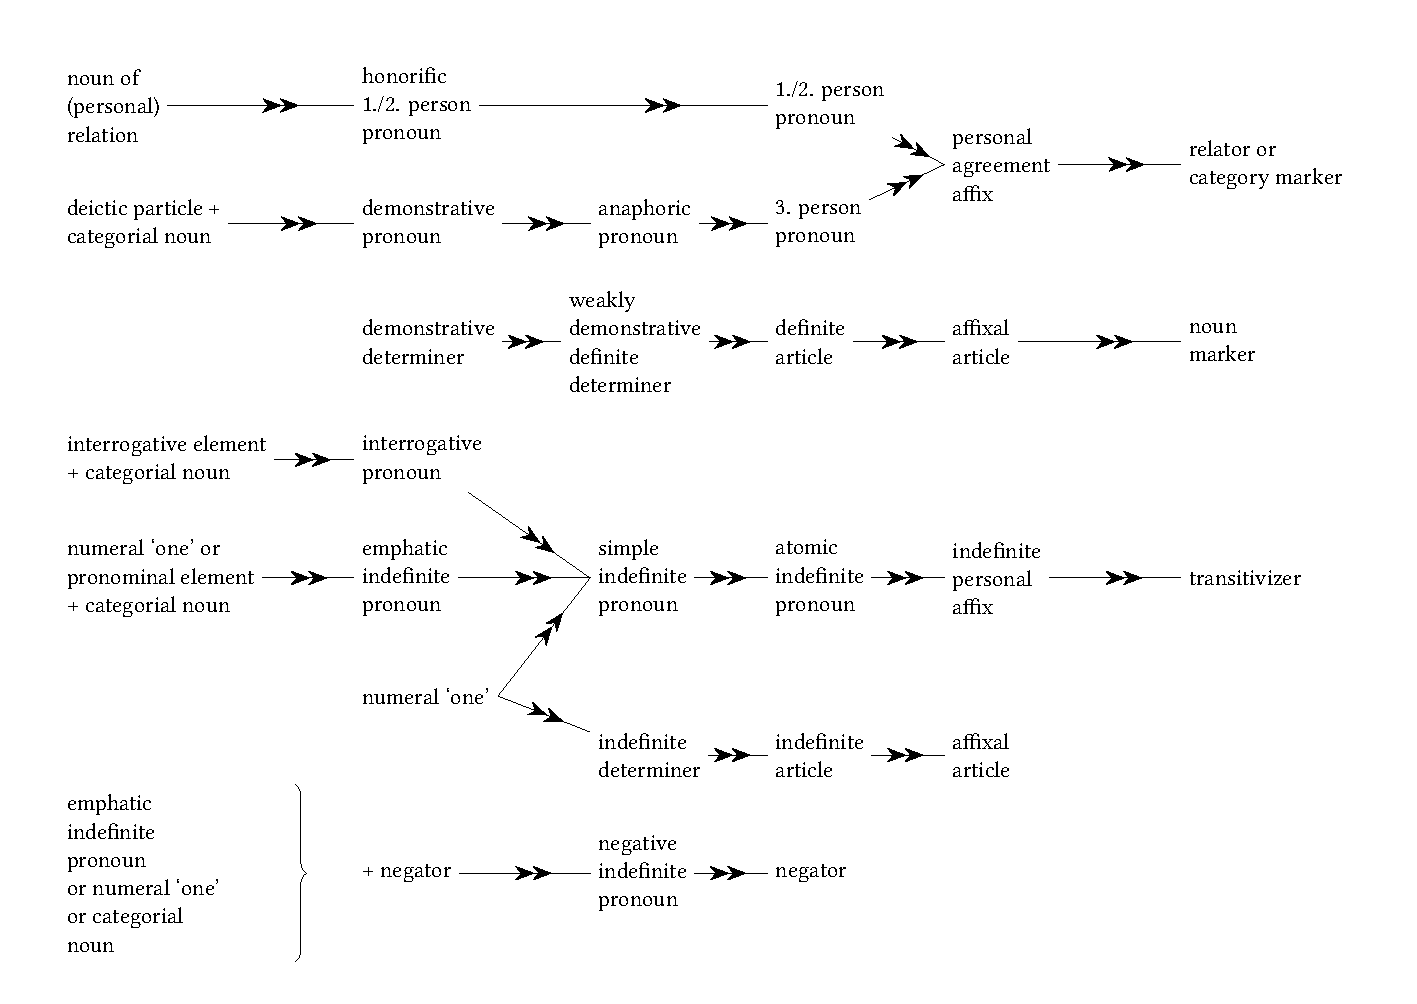
\includegraphics[angle=90, origin=c]{figures/3-Someinterrelatedgramchanels.pdf}
	}
	\caption{Some interrelated grammaticalization channels of pronominal elements} \label{interrelatedpronomel}
\end{figure}
% \REF{ex:F3}.  \textit{Some interrelated grammaticalization channels of pronominal elements}

\subsubsection{Conclusion}
In conclusion of this \sectref{sec:3.2}, we may summarize the various grammaticalization channels of pronominal elements in \figref{interrelatedpronomel} (p.~\pageref{interrelatedpronomel}).
%(\pageref{abc}\chk%49    ) - removed since we can rely on \figref
What has been put in the same column is at the same stage of grammaticalization or has the same degree of grammaticality. Here as in all grammaticalization scales, there are functional similarities between neighbouring positions in a row; but there are also changes which bring it about that the end of a scale may have little in common with the beginning.

There are some open questions here. For instance, in some cases a category developed in the course of grammaticalization is already presupposed at the beginning of the channel. The reader may well wonder about the origin of the elements posited at the beginning of the process. We will defer this troublesome question to §~7.

\section{Nominal complexes}
\subsection{Nominal categories}

Much of what would belong in this section has already been dealt with in the section on the pronoun. Let me briefly repeat the relevant results: Definiteness and indefiniteness affixes on nouns derive from pronouns used as determiners. These may ultimately become mere noun markers.\label{page59} \citet[§~5.3]{Greenberg1978} shows, for instance, that the long vowel in which virtually all nouns in Hausa end may be explained as a former definite article. If such determiners express gender or noun class, then these become, by the agglutination process, categories of the noun.\footnote{As explained above, non-grammaticalizational origins of such nominal categories are conceivable.} Finally, possessive affixes on nouns originate in possessive pronouns which have undergone the agglutination process described in \sectref{sec:3.2.1.2}.

The remaining nominal categories to be treated here are number and numeral classifiers. Case will be left for \sectref{sec:3.4}.

\subsubsection{Number} \label{sec:3.3.1.1}
Languages without a category of nominal number are not rare. When it seems necessary to focus on a group of individuals, many of these can use morphemes of a \textsc{collective} meaning in combination with the noun. An example is Mandarin \textit{men}, which originally meant ‘class’, but is now only used as a collective or plural suffix to human nouns, as in \textit{rénmen} (man-\textsc{Coll}) ‘people’. Similarly, Hixkaryana has a postnominal particle \textit{komo}, which may be appended only to human nouns and other nouns culturally relevant to humans; e.g. \textit{harye komo} (sweet.potato \textsc{Coll}) ‘sweet potatoes’. See also \citet[§~2.1]{Kölver1982a} on so-called nouns of multitude in Bengali and \citet[272]{HeineEtAl1984} on a collective noun meaning ‘kids’ in Boni. All these are enclitic or suffixed to nouns and strictly optional; i.e. the unmarked noun may have a singular or plural meaning.

At the next stage of grammaticalization we get agglutinative number affixes, mostly plural suffixes. The change ‘collective {\textgreater} plural’ is illustrated with historical evidence from Russian, Persian and Arabic in \citealt[52]{Kuryłowicz1965}. Other examples of agglutinative plural suffixes are Turkish -\textit{ler}, Quechua -\textit{kuna} and Yucatec -\textit{o'b}. These vary in degree of optionality, but none is completely obligatory. In the languages enumerated, the plural suffix is at least absent when the noun is accompanied by a numeral.

In \sectref{sec:3.2.1.2} we saw that verbs may acquire the category of number by the agglutination of a personal pronoun. This is also a possible origin of nominal number. We meet here again the two stages just described: first the pronoun accompanies the noun only when there is some special emphasis on plurality; then it becomes affixal and increasingly obligatory. Heine \& \citet[234]{HeineEtAl1984} adduce Yoruba \textit{awɔn} ‘they’, which precedes the noun, as an example of the first stage, and Ewe \textit{wó} id., which is suffixed to the noun, for the second stage. As a result of this, we often find nominal affixes formally similar to third person verb affixes. Compare Yucatec \textit{ch'íich'-o'b} bird-\glpl with \textit{bin-o'b} go-3.\glpl. Mangarayi has \textit{wu-r} \textsc{nonsg-du} and \textit{wu-la} \textsc{nonsg-pl} both as number suffixes to kin terms (other nouns take partly different suffixes) and as pronominal prefixes of third person dual and plural, respectively, to intransitive verbs \citep[88f, 160f]{Merlan1982}.

There is yet a third source of nominal number, and this is numerals and quantifiers. (The three sources are also in \citealt[273]{HeineEtAl1984}). The numerals ‘one’ and ‘two’ may be combined with nouns to yield singular (or singulative) and dual, and a quantifier may provide the plural. In Tok Pisin we get all of these possibilities and in addition a trial. Thus:
\newpage
\ea\label{ex:E24}
\langinfo{\LangTok}{}{~\citep[115, 60]{Mosel1980}}\\
\ea
   dok  \\
\glt ‘a dog, dogs’\\
 wanpela dok \\
\glt ‘one/a dog’\\
\ex tupela dok \\
\glt ‘two dogs’\\
\ex tripela dok \\
\glt ‘three dogs’\\
\ex ol dok \\
\glt ‘(the) dogs’   \\
\z
\z
\noindent The claim that these elements have at least entered the course of grammaticalization may be proved by the fact that \textit{tupela} and \textit{tripela} may also be suffixed to personal pronouns to signify the respective number categories.

Irrespective of their different origins, the three types of number markers have several grammatical properties in common. One of them is their optionality or incomplete obligatoriness, as already mentioned. Furthermore, they are often restricted to human or animate nouns, or these get different affixes from each other or from inanimate nouns. Cf. \citealt[149]{Hewitt1979} on the two number suffixes of Abkhaz. Finally, in this early phase of grammaticalization the paradigm not infrequently comprises more than two numbers. There is a dual in Mangarayi and even a trial in Tok Pisin, and there is a choice among several nouns of multitude in Old Bengali and Hua \citep[221f]{Haiman1980}.

\enlargethispage{1\baselineskip}
As grammaticalization increases, number affixes become completely obligatory and fusional. This stage is characteristic of several ancient Indo-European languages and also some modern ones such as German. The paradigm tends to be reduced to a binary opposition, which is just what we observe in the development from Proto-Indo-European to the historical languages. Number marking is generalized to all nouns in all contexts, and any formal differences among affixes of the same subcategory either disappear or become purely allomorphic, i.e. they lose their semantic motivation. The penultimate stage of grammaticalization of the number distinction is represented by such alternations as \textit{mouse} vs. \textit{mice}, which are more common in Classical Arabic, and by suppletive forms such as Russian \textit{čelovek} vs. \textit{l'udi} ‘man, men’ or \textit{god} vs. \textit{leta} ‘year, years’. The outlet is always that stage where the grammatical marker becomes zero. In nominal number, this is represented by cases such as German \textit{der Wagen} — \textit{die Wagen} ‘the car — the cars’ or English \textit{the fish}.

There is little historical evidence available for this course of events. For the change from the independent to the agglutinative state of the number marker, Bengali (see \citealt{Kölver1982a}) and Chinese are relevant. The evolution from reconstructed Proto-Indo-European to modern German may be taken to evidence the transition from the agglutinative to the fusional and zero stage.

\label{page63}The various grammatical factors which make up every grammaticalization process will be surveyed in \sectref{chap:4}. One of them plays a peculiar role in the development of nominal categories and here appears as the gradual intrusion of the grammatical morpheme into the \np. By this the following is meant: A noun of multitude, personal pronoun or quantifier used as a number marker occurs only once in each \np, normally at its margin. It is a feature of the \np as a whole. With ongoing grammaticalization it may be repeated on the head noun if this does not already carry the marker. This leads to number agreement (and, in the case of the other nominal categories, to gender or case agreement). In this way, number becomes a category of nominal words. A fine example of this phase is Abkhaz; see \citet[222f]{Hewitt1979}. At the end of the process, number again disappears from non-nuclear subconstituents, ending up as a category of the noun. This is largely true of English. For details see \citealt[§~6.3]{Lehmann1982b}; for the parallel development of case marking see p. \pageref{page92}\chk%76
  below.

We will only touch upon one phenomenon which is very frequent in the development of number marking, but whose counterparts occur throughout the grammar: the paradigm is often simplified by generalizing one allomorph to the detriment of the others. This is particularly common when grammaticalization is already far advanced. Thus, the plural in -\textit{s} has been generalized to practically all nouns in English and in Spanish, though at earlier stages of the languages there had been much irregularity. However, whereas in the above cases a reduction of the paradigm, i.e. of the semantically distinct subcategories, was observed, here we face a reduction of allomorphy. These two processes are to be clearly distinguished, and we shall see in \sectref{sec:4.2.2} that only one of them is a defining characteristic of grammaticalization.

\subsubsection{Numeral classifiers}
Morphemes which express the lexical class into which a noun belongs may be combined with any of its determiners or attributes. According to the category that they attach to, we distinguish between article, possessive and numeral classifiers. Since very little is known about the first two types, I will not treat them here (see \citealt[§~6.3.3]{Lehmann1982b} for some discussion). For detailed information on numeral classifiers, see \citealt{Kölver1982b} and \citealt{Serzisko1980,Serzisko1982}.

The Indo-European languages originally had no classifiers. In modern Persian (Farsi, \citealt{Moinfar1980}), nouns may still be accompanied by a bare numeral, as in \textit{do \=ir\=an\=i} `two Iranians'. The noun is always in the singular. Alternatively, however, we may bestow a classifier on the numeral and form \textit{do nafar \=ir\=an\=i} (two person Iranian). The optionality of the pattern points to its relatively weak grammaticality, as does the size of the paradigm, which consists of 14 classifiers.\footnote{This is not a very reliable criterion, as we shall see in \sectref{sec:4.2.2}. In the case of numeral classifiers, one must be warned that the figures given in the literature on various languages are often greatly exaggerated, because mensuratives, which designate portions of masses or form collections, are counted as classifiers.} All of them derive from nouns, whose lexical meanings are still perfectly transparent, and all but two can still be used as nouns. They remain free forms in the numerative construction, and no sandhi phenomena occur. On the other hand, several features indicate that the classifiers are already grammaticalized to a certain degree. First, the paradigm is tightly integrated and hierarchically organized. There are eight forms for different classes of inanimate objects, one for bigger and domestic animals, two for smaller animals and inanimate objects which neutralize the first eight, two for human beings, and one universal classifier which neutralizes all the others. Secondly, although the ``Grundbedeutungen'' of the classifiers are transparent, some of these do not fit the classifier use. For instance, \textit{dast} means ‘hand’ but is used in, e.g. \textit{yek dast leb\=as} (one hand clothing) ‘one suit’. The grammatical correlate of this desemanticization is the fact that the construction is not syntactically treated as one of nominal modification, with the classifier as the head noun. If it were, the attributor (izafat) -\textit{e} would have to be appended to the classifier (cf. \sectref{sec:3.3.3}), which it never is. In short, what we have here is a weakly grammaticalized system of numeral classification.

Contrast this with the Japanese classifier system. First of all, there are two series of numerals, one of native Japanese origin, the other borrowed from Chinese. Some classifiers combine with one number series, some with the other series, with no interchange possible. Apart from those classifiers which represent objects directly counted, such as money and time units, there are only five classifiers in general use: two of Japanese origin for humans and non-humans, and three of Chinese origin for different kinds of objects. Classifiers are completely obligatory; it is impossible to count objects without an intervening classifier. None of the classifiers has an independent use or a meaning of its own. They are suffixed to the numerals, and this is accompanied by assimilations of great irregularity. For instance, \textit{hati} ‘eight’ + -\textit{hon} ‘long, cylindrical object’ yields \textit{happon}, whereas with -\textit{satu} ‘bound object’ it yields \textit{hassatu}. The system is further complicated by the fact that some numerals have allomorphs whose distribution is determined by the following classifier, and vice versa: some classifiers have allomorphs whose distribution is determined by the preceding numeral. This is clearly a strongly grammaticalized classifier system.

Mandarin Chinese has long had a classifier system, which formerly had been, and in the written style still is, fairly differentiated. The classifiers are suffixed to the numeral. In the modern spoken language, the Mandarin dialect, the system is reduced to what had been the most general classifier, -\textit{ge}. Furthermore, the combination \textit{yí-ge} (one-\textsc{cl}) may be reduced to \textit{ge}, whereby \textit{ge} assumes the meaning of unity. Its use has also been generalized to demonstrative pronouns, and here it functions as a marker of singularity. At this stage, it means no more than ‘individual, unit’ (cf. \citealt[24f]{Serzisko1980}). This is the end of the grammaticalization of a numeral classifier system.

\label{page65}One feature that characterizes classifier systems to a varying degree is the paradigmatic variability of the classifier (see especially \citealt{Serzisko1982}). Suppose a noun has a constant, inherent classifier corresponding to its lexical class. Normally this may be substituted by a more general, unmarked classifier, but this is not paradigmatic variability. What is meant by this term in numeral classification is the discretionary combination of a noun with a classifier neither inherent to it nor hierarchically superordinate, by which it is, for the moment, allocated to a different class. The following examples are from Burmese (s. \citealt[20]{Serzisko1980}). The noun \textit{myiʔ} ‘river’ is inherently classified by itself, yielding the repeater construction \textit{myiʔ tə myiʔ} ‘one river’, where the order is ‘noun numeral classifier’. However, the classifier may alternatively be \textit{yaʔ} (\cl.place), if we refer to the river as, for instance, a place for a picnic; or \textit{tan} (\cl.line), meaning, for instance, a river on a map; or \textit{'pa} (\cl.sacred object) in dealing with mythological rivers. This wrong, as it were, classification of a noun is used in various languages for jocular or derogatory effects and points to the relative freedom of the speaker vis-à-vis the system. Paradigmatic variability is more likely among free forms than among bound forms. We may therefore say that it decreases with increasing grammaticalization.

\subsection{Nominalization} \label{sec:3.3.2}

Viewed syntactically, nominalization is the transposition of a clause into a noun; viewed semantically, it is the transposition of a proposition into a concept. As there is a great distance between the two poles of this transition, there are many stages in between, which correspond to different degrees of grammaticalization of the construction. Since I have treated nominalization more comprehensively in \citealt{Lehmann1982a}, I will here exemplify only some of these stages in order to make the principle apparent.

In Chinese, both classical and modern Mandarin, subject and object complement clauses may be embedded without any sign of subordination, as in \REF{ex:E25} from Mandarin.

\ea\label{ex:E25}
\langinfo{\LangMand}{}{~\citep[38]{Bossong1979}}\\
\gll   t\=a  s\v{i}-le  w\v{o}  zh\=en  nán-shòu\\
 he  die-\textsc{pf}  I  very  sad\\
\glt {‘I am very sad that he has died.’}\\
\z
\noindent Similar constructions are frequent in English, where we have \textit{I bet (that) he wins}, with or without the subordinator. There is no structural difference between the embedded and an independent clause, the only hint for the embedding being the syntactic function of the dependent clause as an \np in the superordinate clause. This is why we recognize nominalization here.

The development of subordinators from other conjunctions will be treated on p.~\pageref{page70}\chk%58
 . Apart from this, there are two main sources of subordinative conjunctions which serve to embed clauses. The first may be exemplified by English \textit{that}, German \textit{daß}, Welsh \textit{a}, Accadic \textit{ša} ({\textless} \textit{šu}) and Nahuatl \textit{in}. Here a \textsc{demonstrative} is used to announce the embedded clause. Then a mechanism sets in which prescribes that whatever is preceded (or followed, as the case may be) by a demonstrative as a coconstituent must be a nominal. So the embedded clause is perforce nominalized, and the demonstrative degenerates to a mere subordinator.

The second source of subordinators are \textsc{verba dicendi}. Their grammaticalization to subordinators has been studied in \citet{Lord1976}. Ewe has several such verbs, one of them, \textit{bé}, governing indirect speech as in \REF{ex:E26}.

\ea\label{ex:E26}
\langinfo{Ewe}{}{~\citep[179]{Lord1976}}\\
\gll me-be 
 me-wɔ-e.\\
 I-say  I-do-it\\
\glt {‘I said (that) I did it.’}\\
\z
\noindent Subsequently, this verb is used to introduce indirect speech after verbs which cannot govern it, in a type of construction such as ‘I argued that it is wrong.’ At a further stage of grammaticalization, the indirect speech condition is dropped, and \textit{bé} is used to introduce all types of object clauses, then all types of complement clauses, yielding sentences such as \REF{ex:E27}.

\newpage
\ea\label{ex:E27}
\langinfo{Ewe}{}{~\citep[180]{Lord1976}}\\
\gll me-dí  bé  má-ɸle  awua  ɖewó.\\
 I-want  \textsc{sr}  I:\textsc{sbjv}-buy  dress  some\\
\glt {‘I want to buy some dresses.’}\\
\z
\noindent \textit{Bé} now has become a complementizer. In such constructions, it no longer behaves like a verb; it takes, for instance, no verbal affixes. Lord adduces similar examples from Efik and Yoruba.

The weak degree of grammaticality of these two types of subordinators is obvious from several facts. They are full words, forming a constituent of their own and not particularly attached to any specific constituent of the subordinate clause. Their etymological meaning is perfectly transparent. In the better known cases (English, German), the subordinator enters into a paradigm with a host of conjunctions which take the same position but differ from it in meaning. Note the optionality of \textit{that} in some contexts.

If the subordinator, instead of preceding the dependent clause, comes at its end, the construction is slightly more grammaticalized. This may be observed in Japanese, as in \REF{ex:E28}.

\newcommand\jpn[1]{\raisebox{-.45cm}{#1}}
\ea\label{ex:E28}
\langinfo{\LangJap}{}{~\citep{Kuno1973}} \\
\gll Ano  hito  {$\left\{\begin{array}{c}\text{ga}\\\text{no}\end{array}\right\}$} hon  o  kai-ta  koto  ga  yoku  sirarete  iru. \\
\jpn{that}  \jpn{person}  {$\left\{\begin{array}{c}\text{\textsc{nom}}\\\text{\glgen} \end{array}\right\}$}  \jpn{book}  \jpn{\textsc{acc}}  \jpn{write-\textsc{past}}  \jpn{\textsc{nr}}  \jpn{\textsc{nom}}  \jpn{well}  \jpn{known}  \jpn{is}\\
\glt {‘That that person has written a book is well known.’}\\
\z
\noindent The etymological meaning of the subordinator \textit{koto} ‘thing’ is still recoverable. It is an independent word and constitutes a paradigm with several other subordinators which can appear in its position (e.g. \textit{no}; cf. p.~\pageref{page74}\chk%61
f  below). However, the construction is slightly more grammaticalized than the English one, as may be seen by the following criteria. Firstly, the subordinator of complement clauses is non-omissible. Secondly, the construction may be followed by a case particle (\textit{ga} in \REF{ex:E28}), indicating that syntactically it is treated like any \np. Thirdly, the verbal paradigm of the subordinate clause is reduced, several modal and honorific forms being excluded from it. Lastly, the subject of the subordinate clause may not only be in the nominative, but alternatively in the genitive. On a typological scale, this mostly occurs only if the subordinate verb itself is nominalized (cf. also \citealt[39]{Bossong1979}), which is clearly not the case in \REF{ex:E28}. However, diachronic considerations \citep[45--47]{Bossong1979} make it plausible that the genitive in subordinate clauses such as \REF{ex:E28} is a holdover from an earlier embedding construction where the verb did have a nominal form.

At the next stage of grammaticalization, the subordinator becomes affixal, and the subject of the nominalized clause regularly goes into the genitive, as in \REF{ex:E29}.

\xbox{\textwidth}{
\ea\label{ex:E29}
\langinfo{\LangTurk}{}{~\citep[187]{Wendt1972}} \\
\gll Anne-n-in  gel-mey-eceğ-i-ni  söyle-di.\\
{mother-your-\glgen}  come-\textsc{neg}-\textsc{nr}.\textsc{fut}-her-\textsc{acc}  say-\textsc{past}\\
\glt {‘He said that your mother will not come.’}\\
\z
}
\noindent There is only one more nominalizer in Turkish which functions like the one in \REF{ex:E29}, and it indicates non-future. Neither has an independent meaning. Both of them occupy the position of the verbal tense suffix, thus reducing the tense paradigm to a binary opposition. The subject-predicate syntagm of the nominalized clause is maximally likened to a genitive-head noun syntagm, since not only does the subject have a genitive suffix, but also the nominalized verb has an obligatory possessive suffix referring back to the subject. Nevertheless, we do not yet have a deverbal derived noun here; the formation of \REF{ex:E29} is entirely a matter of syntax.

However, the next step in the grammaticalization scale does lead us to \textsc{verbal nouns} which retain few of the properties of the full clause which we started from. English nominalizations in -\textit{ing} are an example. Here it is clear that we are dealing with the nominalization not of a clause, but of a verb. The suffix constitutes a one-member paradigm of nominalizers and cancels all the verbal categories of English. Still, the verbal noun may take arguments and adjuncts almost like the finite verb of a clause. The subject is, of course, in the genitive. In the other modifiers, there is an interesting variation: the object may either remain in the accusative, or it may pass into the genitive, too. In the first alternative, adverbs remain such, whereas in the second alternative they become adjective attributes to the verbal noun. A third correlating phenomenon is the possibility of an article in the latter, but not in the former case. Thus:

\ea\label{ex:E30}
\langinfo{\LangEngl}{}{} \\
\ea John's constantly reading magazines
\ex John's constant reading of magazines
\ex *the (constantly) reading magazines
\ex the (constant) reading of magazines\\
\z
\z
\noindent So we have two stages of our grammaticalization scale embodied in the English \glposs-\textit{ing} construction. At the latter stage, the nominalized verb has assumed all the relevant features of a noun; -\textit{ing}{}-nominalizations are even pluralizable.

Extreme grammaticalization leads to the deletion of the grammatical formative. In nominalization, we would be looking for \textsc{conversion} of verbs into nouns without an overt derivative affix. Examples are, of course, known from English: \textit{to run — the run, to love — the love}, etc. However, while virtually all verbs can be nominalized by the -\textit{ing} suffix, most verbs cannot be nominalized by a zero affix. There is a restriction of productivity here which we have so far not found to be typical of grammaticalization. I will return in §~5.2 to a conception which can accommodate these heterogeneous facts, and try here another example which apparently does not present this complicating factor. Nominalizations similar to the ones just cited from English are common in Classical Chinese; cf. the following example from Su Shi:

\ea\label{ex:E31}
\langinfo{\LangMand}{}{~\citep[40]{Bossong1979}}\\
 \ea
 \gll b\=ing  bù  kě  qù.\\
 soldier  not  can  leave\\
\glt {‘Military is indispensable.’}

\ex
\gll xi\=an  wáng  zh\v{i}  b\=ing  zh\v{i}  bù  kě  qù.\\
   former  king  know  [soldier  \glgen  not  can  leave]\\
\glt {‘The former kings were aware of the indispensability of the military.’}
\z
\z
\noindent There is only an indirect sign of nominality of the verb phrase \textit{bù kě qù} in \REF{ex:E31}.b, viz. the genitive particle following its semantic subject. We must therefore assume nominalization by a zero affix to have taken place; and this is in fact such a common process in classical Chinese that earlier scholars (e.g. \citealt{Misteli1893}) had diagnosed a random shift of word classes or, equivalently, the total lack thereof. However, on the basis of facts about grammaticalization that we have seen up to now, the technique exemplified by \REF{ex:E31} fits in the scale as representing an expectable, if extreme, degree of grammaticality of nominalization. There arises, however, the further problem that the difference of nominalizations as exemplified by \REF{ex:E31} and such others as exemplified above by \REF{ex:E25}, which we have posited at opposite ends of the grammaticalization scale, appears to be minimal. This will be dealt with in \sectref{sec:4.4.4}.

The renovation of a nominalizing construction may be either complete or partial. We may call it complete if no feature of an inherited nominalizing construction is used in the renovation. This has happened during the change from classical to modern Japanese (see \citealt[45f]{Bossong1979}). Classical Japanese had an infinite verb form which was used in nominalizations. By phonological and morphological change, this became indistinguishable from the “finite” main clause verb form, and nominalization was renewed by means of postposed particles of nominal origin, as exemplified in \REF{ex:E28}. A complete renovation is also the substitution of the Latin accusativus-cum-infinitivo construction by clauses subordinated with the help of \textit{que/che} in the Romance languages.

In partial renovation, only the subordinator is renewed. This process, which is very common in Indo-European languages, was already studied by \citet{Meillet1915}. Typically, a subordinate clause introduced by the unmarked subordinator (English \textit{that}, German \textit{daß}, Romance \textit{que/che}, Persian \textit{ke}, Turkish -\textit{diğ}{}-, etc.) is embedded as the complement to a noun or a preposition. Then either this head coalesces with the subordinator, or the subordinator becomes dispensable, the former head becoming the new subordinator. Examples are Italian \textit{dal momento che} ‘since’, French \textit{parce que} ‘because’, \textit{puisque} ‘since’, \textit{avant que} ‘before’, Turkish -\textit{diğ}-\glposs \textit{zaman/hal-de} (-\nr-\glposs time/ state-\glloc) ‘when/although’. The former subordinator has disappeared in English \textit{before}, German \textit{bevor} and \textit{fall-s} (case-\advr) ‘if’.

The \textsc{making of conjunctions} would easily fill a whole book. The process by which local conjunctions become temporal ones and temporal conjunctions become causal, conditional etc. conjunctions, is also a sort of grammaticalization (see §~5.1). Examples are German \textit{da} ‘at the place where’ {\textgreater} ‘at the time when’ {\textgreater} ‘by the reason that’, Engl. \textit{since} ‘from the time that’ {\textgreater} ‘from the reason that’, Ital. \textit{dal momento che} id., \textit{qualora} (which:hour{\textgreater}) ‘if’.\label{page70} In the end, conjunctions which mark a semantic relation of the subordinate to the main clause are grammaticalized to mere subordinators, as when Latin \textit{quod} and \textit{quia} ‘because’ both fuse into Romance \textit{que/che} ‘that’. The same phenomena repeat themselves in the prepositions.

In contradistinction to this evidence of renovation of conjunctions, evidence for their reinforcement is somewhat scant. Possibly French \textit{parce que}, adduced above as an example of renovation, is rather one of reinforcement. This depends on whether the \textit{que}{}-clause, at the time it was combined with \textit{par ce}, was a mere complement clause (as assumed above) or a causal clause. The parallel case of German \textit{da} {\textgreater} \textit{zumal da} {\textgreater} \textit{zumal} ‘since’ is somewhat more convincing.

Clearer evidence comes from subordinators derived from verba dicendi \citep[183]{Lord1976}. In Efik and Yoruba, the subordinator \textit{ke}, which comes from a verb meaning ‘say’, has been reinforced by a second subordinator \textit{ete}, of the same provenience. Example:

\xbox{\textwidth}{
\ea\label{ex:}
\langinfo{Efik}{}{~(after \citealt[183]{Lord1976})}\\
\gll Kristian  ɔdɔhɔ  ete  ke  imɔ  idi  idikɔ  owo...\\
 K.  say  \textsc{sr}  \textsc{sr}  he  \textsc{cop}  man  wicked\\
\glt {‘Kristian says that he was a wicked man...’}\\
\z
}
\noindent The more recent subordinator then tends to dispense with the former one, just as in some of the above examples of renovation. Similar observations apply to the Abkhaz particle \textit{\=h°a}, which stems from a verb meaning ‘say’ and develops into a general subordinator (cf. \citealt[5--8, 28--35, 43]{Hewitt1979}).

A few words must be said about nominalizations in which an argument place — mostly the subject position — of the infinite verb must be left open, so that it can be semantically filled, with the help of syntactic rules, by an \np of the main clause. The \textsc{infinitives} which appear in this function are very often embedded by a particle or affix which derives from a directional adposition. Examples are English \textit{to}, German \textit{zu}, Romance \textit{a}, Swahili \textit{ku}{}- (cf. \citealt{Meinhof1936}) and the case suffixes, mostly the dative (s. \citealt[298]{Szemerényi1970}), on Sanskrit infinitival verbal nouns. This is naturally explicable by the final function which infinitival complements usually have at their origin. Similarly, gerundial suffixes are often based on locative markers; cf. what was said on p.~\pageref{page33}\chk%26
on periphrastic progressive aspects. Once a verb form is embedded with the help of such a directional or local marker, the same process as noted above for the demonstrative subordinators takes place: since that which is the complement to an adposition or even a case affix must be of a nominal nature, these signs will suffice to express the nominalization and degenerate to mere nominalizers. This is easily shown for English \textit{to} = German \textit{zu}, which can even introduce infinitivals in subject function.

Certain types of nominalized clauses derive from the combination of an \np of the main clause with an infinitival complement whose subject place the former fills. Thus, there is unanimity among scholars that the Latin \textsc{accusativus cum infinitivo} originated in sentences such as \REF{ex:E33}.

\ea\label{ex:E33}
\langinfo{Latin}{}{}\\
\gll Petrus  videt  Paulum  currere.\\
 {Peter:\textsc{nom}.\glsg}  {see:3.\glsg}  {Paul:\textsc{acc}.\glsg}  {run:\glinf}\\
\glt {‘Peter sees Paul run(ning)’}\\
\z
\noindent \xbox{\textwidth}{
\ea\label{ex:E34}
\langinfo{Latin}{}{} \\
\gll Carthaginem  deleri  necesse  est.\\
{Carthago:\textsc{acc}.\glsg}  destroy:\glinf.\textsc{pass}  necessary  is\\
\glt {‘It is necessary that Carthago be destroyed.’}\\
\z
}
\noindent There \textit{Paulum} is the object of the main clause. Its subjecthood vis-à-vis the infinitive at this initial stage is a consequence of a semantosyntactic rule of complex sentence structure. Subsequently, its subject status becomes grammaticalized, and we also get a.c.i. in non-object positions of the main clause, as in \REF{ex:E34}.

\REF{ex:E34} might also be expressed in English by \textit{It is necessary for Carthago to be destroyed}. Here we have another subtype of the complement clause originating in the combination of an \np of the main clause with an infinitival complement whose subject position it fills (see \citealt[300--306]{Jespersen1940} on details). While in American English the grammaticalization of this construction is already far advanced, in French it has come up recently and is still classified as ‘faute’ in \citealt[94]{Frei1929}. Frei's examples are:

\ea\label{ex:E35}
\langinfo{\LangFren}{}{} \\
\ea
  m'envoyez son adresse pour moi lui écrire\\
\glt ‘send me his address so I may write him’\\
\ex Où trouver l'argent pour lui voyager?
\glt ‘Where (may I) find the money for him to travel?’
\ex Ci-joint un timbre pour vous avoir la bonté de répondre.
\glt ‘Here enclosed a stamp for you to be so kind as to answer.’
\z
\z
\noindent These examples show very clearly the conditions under which the construction originates: The subsequent subordinate subject must be a beneficiary in the main clause, which is adjoined with the help of the preposition ‘for’. The infinitive complement must express the action which the beneficiary is expected to be able to accomplish with the help of the benefaction and which, being a purpose or consequence of the main clause action, is introduced by the final preposition ‘to’. In the course of grammaticalization, these semantic conditions are gradually weakened or dropped, and the erstwhile beneficiary \np of the main clause becomes the subject of the infinite clause. This may go so far that the subordinate subject is even put into the nominative.\label{page72} Modern Portuguese has reached this advanced stage of grammaticalization of the ‘for-to’ complement clause, as exemplified in \REF{ex:E36}.

\ea\label{ex:E36}
\langinfo{\LangPort}{}{} \\
\gll Ele  trouxe  um  livro  para  eu  ler.\\
he  brought  a  book  for  I  read:\glinf\\
\z
\noindent The construction from which \REF{ex:E36} must have arisen, namely \textit{Ele trouxe um livro para mim ler} (\textit{mim} ‘me’), is nowadays even condemned by the grammarians, though it is still current in the colloquial language.

\label{page73}While infinitival complements may, thus, contribute to form a full complement clause, the reverse process, the reduction of a clause whose argument positions are all filled to a relational infinitival complement which has necessarily an unoccupied argument position, has not been observed. Recall that this is certainly not what is at stake in the grammaticalization process leading from \REF{ex:E25} to \REF{ex:E31}.b above. It appears that the opening of an argument position is not something which comes about by grammaticalization. Therefore, while we often do have paraphrases among \textit{that}{}-clauses, \textit{for-to} nominalizations and -\textit{ing}{}-nominalization, \textit{that}{}-clauses can practically never be used as a paraphrase of an infinitive complement. Consider the infinitive complement in sentences such as \textit{I let him go} or \textit{forced him to go}. The main verb does not leave the possibility of its direct object being different from the semantic subject of the subordinate verb. Therefore, the subject position of the latter must remain unfilled.

\subsection{Attribution} \label{sec:3.3.3}

We will treat here two kinds of attributes, adjective attributes and possessive attributes, traditionally called genitive attributes. Quite a few languages use an attributor, a relational particle, in the combination of either kind of attribute with a head noun. \REF{ex:E37} shows a genitive attributor, \REF{ex:E38}f show relators which may attribute either an \np (a) or an adjectival (b) to the head noun.

\ea\label{ex:E37}
\langinfo{\LangJap}{}{}\\
\gll watakusi  no  hon  \\
 I  \textsc{at}  book\\
\glt   ‘my book’
\z
\noindent \ea\label{ex:E38}
\langinfo{\LangMand}{}{}  \\
 \ea
 \gll  w\v{o}  de  sh\=u  \\
 I  \textsc{at}  book  \\
\glt ‘my book’\\
\ex
\gll  yàojin  de  huà  \\
 important  \textsc{at}  discourse \\
 \glt ‘important words’\\
\z
\z
\noindent  \ea\label{ex:E39}
 \langinfo{Persian}{}{}   \\
 \ea
 \gll  ket\=ab  {}-e  man  \\
book  {}-\textsc{at}  I \\
\glt ‘my book’\\
\ex
\gll  d\=al\=an  {}-e  der\=az  \\
 corridor  {}-\textsc{at}  long\\
 \glt 
 ‘long corridor’\\
\z
\z
\noindent One development which can lead to such constructions is the grammaticalization of \textsc{anaphoric} or substantivized \textsc{attributes}. When a concept (not a referent) is (pronominally or implicitly) resumed in lexical anaphora and combined with a (new) attribute in order to identify a referent, we have an anaphoric attribute. In English, \textit{one} is used as the anaphoric head in such cases.\label{page74} Japanese has a polyfunctional particle \textit{no}. Its former lexical meaning was ‘matter, fact, case’ \citep[99]{Jorden1962}. It functions as the grammatical head noun in lexical anaphora, as in \REF{ex:E40}. 

\ea\label{ex:E40}
\langinfo{\LangJap}{}{} \\
 \ea
 \gll Dare  no  hon  desu  ka?  ---  Watakusi  no  desu.\\
  who  \textsc{at}  book  \textsc{cop}  \textsc{int}  {}  I  \textsc{at}  \textsc{cop}\\
\glt {‘Whose book is it?’} ---  {‘It is mine.’}\\
\ex
\gll  Dono  hon  desu  ka?  ---  Atarasii  no  desu.\\
 which  book \textsc{cop}  \textsc{int}  {} new  \textsc{at}  \textsc{cop}\\
\glt {‘Which book is it?’} --- {‘It is the new one.’}\\
\z
\z 
\noindent\label{page74b}\textit{No} may also be a nominalizer; in this function it may be substituted for \textit{koto} in \REF{ex:E28} above. We may assume it to have taken the following development: The ``Grundbedeutung'' of a construction ‘X \textit{no}’ is ‘the thing characterized by X’. In this construction, X can be either a — possessive or adjective — attribute, as in the answers of \REF{ex:E40}, or an embedded clause, as in the altered version of \REF{ex:E28}. The attributive function of \textit{no}, as in \REF{ex:E37}, is a secondary development. \REF{ex:E37} represents the grammaticalization of the appositive combination of a substantivized attribute with a lexical head; its original meaning is ‘my thing, the book’. In this way, an older (optionally asyndetic) possessive attribution was renewed. A parallel renovation of adjective attribution did not take place, because adjectives are marked as attributes by their desinence -\textit{i} (cf.~\REF{ex:E40}b).

\label{page75}Similar constructions involving nouns with the meaning ‘thing’ or ‘possession’ are elsewhere frequent in the expression of alienable possession. A further example is the possessive \np in Thai (see \citealt[389]{MallinsonEtAl1981}). It has the form ‘possessum \textit{khɔɔŋ} possessor’. \textit{Khɔɔŋ}, now a preposition, comes from a noun meaning ‘thing, goods, possessions’. Many languages, among them Bororo, Bambara and Dyula, have an attributor of alienable possession that stems from an inalienable noun.

A similar renovation of a juxtaposed attribute by an anaphoric one may be posited for Mandarin Chinese. Besides \REF{ex:E38}b, we have \textit{jàojin huà}, with the same meaning, but less emphasis on the attribute. On the other hand, we have anaphoric or substantivized attributes with \textit{de}, as in \textit{shì yàojin de} ‘is (an) important (one)’. An older form of \textit{de} is \textit{zhi}, as exemplified in \REF{ex:E31}b above. This is known to have been a demonstrative (cf. the \textit{shì} in \sectref{sec:3.1.2} above). It is therefore safe to assume that attribution by means of \textit{de} results from an emphatic renovation of the earlier, still subsisting, juxtapositive attribution.

The history of the Persian attributor (izafat) is better known (cf. \citealt[Ch.~\textsc{vi}.3]{Lehmann1984} and the literature cited there). Old Persian and Avestic had a relative pronoun \textit{hya}{}- or \textit{ya}{}-, respectively, which, apart from introducing ordinary relative clauses, was also used in the formation of nominal attributes, as in \REF{ex:E41}.

\ea\label{ex:E41}
\langinfo{\LangAvest}{}{} \\
\ea
\langinfo{}{}{(Yt.10, 65)}\\ 
\gll \=aa  ya  mî${\circleddash}$rəm  yim  vouru-gaoyaoit\=im fr\=adam  azəm\\
then  \textsc{sr}  Mithra:\textsc{acc}.\glsg.\textsc{m}  \textsc{rel}:\textsc{acc}.\glsg.\textsc{m}  ample:pasturage:\textsc{acc}.\glsg.\textsc{m} {created:1.\glsg}  I\\
\glt {‘when I created Mithra, the one with ample pasture lands’}\\
\ex
\langinfo{}{}{(Vd. 5,1)}\\
\gll  tam  kəhrpəm  fraŋuharaiti yam  iristahe  mašyehe\\
   \textsc{det}:\textsc{acc}.\glsg.\textsc{f}  body:\textsc{acc}.\glsg.\textsc{f}  {eat:3.\glsg}    \textsc{rel}:\textsc{acc}.\glsg.\textsc{f}  deceased:\glgen.\glsg.\textsc{m}  man:\glgen.\glsg.\textsc{m}\\
\glt {‘he eats the body of the dead man’}\\
\z
\z
\noindent Originally, these were nominal relative clauses, with the relative pronoun as the subject. They forfeit this status, however, as soon as the relative pronoun, instead of being in the nominative, agrees with the head noun in case (as does the nominal predicate), as it does in the examples. At this stage, the relative pronoun becomes a mere attributor, though one distinguished from those discussed so far by its agreement. This, however, is subsequently lost, so that the attributor becomes identical to the subordinator also to be seen in \REF{ex:E41}a. Example:

\ea\label{ex:E42}
\langinfo{\LangAvest}{}{~(V. 5,39)}\\
 \gll mi  aŋhv\=o  ya  astvainti\\
 \textsc{dem}:\textsc{lok}.\glsg.\textsc{m}  life:\textsc{lok}.\glsg.\textsc{m}  \textsc{at}  bodily:\textsc{lok}.\glsg.\textsc{m}\\
\glt {‘in this worldly life’}\\
\z
\noindent This emphatic attribution gradually gains ground against the inherited juxtapositive attribution, concomitantly with the loss of the agreement of the attribute. The inherited construction is then almost ousted, while the attributor is further reduced phonologically and becomes a suffix of the head noun. The emphatic force of the construction is also lost, and the result is to be seen in \REF{ex:E39}.

The Persian case is somewhat different from the Japanese and Chinese ones, as in these certainly no relative pronoun is involved. Their common feature is, however, that the resulting attributor comes from a noun anaphorically related to the subsequent head noun of the attribution and representing this vis-à-vis the attribute. This hypothesis provides a natural explanation for the otherwise startling formal identity of the attributor and the nominalizer in some of the above languages as well as several others, e.g. Lahu. It is, I think, the only way to make sense of the phenomenon that an adjective or a possessor noun should need a nominalizer in order to be attributable to a head noun (the alternative, that a dependent clause should receive an attributor in order to become nominalized, makes no sense, anyway).

An anaphoric pronoun which serves as the head of an anaphoric or substantivized attribute may, of course, show gender or noun class agreement with its repraesentatum. When this construction is apposed to the repraesentatum as the head noun, we have agreement of the attributor with the head noun just as in \REF{ex:E41}. An example is Gothic \textit{hardeis sa goda} (shepherd:\textsc{\glnom.\glsg.\glm} that.\textsc{\glnom.\glsg.\glm} good:\textsc{\glnom.\glsg.\glm}) as against \textit{hairdeis gods} (good:\textsc{\glnom.\glsg.\glm}) (with weak and strong adjective declension, respectively; see \citealt[110]{Ramat1980}). Both constructions mean ‘the good shepherd’; the former is emphatic and more recent, the latter inherited and neutral. While in Gothic the demonstrative has not become an attributor, but an article, its fate was different in the Bantu languages (details in \citealt[§~7.2]{Lehmann1982b}). In Swahili we find an attributor which agrees with the head noun in noun class. The possessive attribute construction is [~\textsc{clx}-head~[~\textsc{clx}-\textsc{at} \textsc{cly}-attribute~]~]. Examples:

\ea\label{ex:E43}
\langinfo{\LangSwah}{}{~\citep[275]{Welmers1973}} \\
 \ea
 \gll  ki-su  ch-a  Hamisi\\
  \textsc{cl}\oldstylenums{7}-knife  \textsc{cl}\oldstylenums{7}-\textsc{at}  Hamisi\\
\glt {‘Hamisi's knife’}\\
\ex
\gll  ny-umba  y-a  m-tu  yu-le\\
\textsc{cl}\oldstylenums{9}-house  \textsc{cl}\oldstylenums{9}-\textsc{at}  \textsc{cl}1-man  \textsc{cl}\oldstylenums{1}-that\\
\glt {‘that person's house’}\\
\z
\z 
%\setcounter{page}{1}
\noindent From the origin of the construction as posited, the attributor is a coconstituent of the attribute. It becomes clitic to the attribute; and further grammaticalization, which may be observed in the related language Tswana, leads to its prefixation, as in \REF{ex:E44}.

\ea\label{ex:E44}
\langinfo{\LangTswa}{}{~\citep[160]{Cole1955}}\\
\gll    mo-sadi  w-a+mo-tšomi\\
 \textsc{cl}\oldstylenums{1}.\glsg-woman  \textsc{cl}\oldstylenums{1}.\glsg-\textsc{at}+\textsc{cl}\oldstylenums{1}.\glsg-hunter\\
\glt {‘the wife of the hunter’}\\
\z
\noindent Here the possessive attribute agrees with its head noun in noun class. Possessive attributes are thus treated structurally exactly as adjective attributes, which agree with their head noun by similar prefixes:

\ea\label{ex:E45}
\langinfo{\LangTswa}{}{~\citep[140]{Cole1955}}\\
\gll     mo-sadi  yômo-ntlê\\
 \textsc{cl}\oldstylenums{1}.\glsg-woman  \textsc{cl}\oldstylenums{1}.\glsg-beautiful\\
\glt {‘a beautiful woman’}\\
\z
\noindent \label{page77}On the basis of the facts discussed so far, I venture the hypothesis that the agreement of the — possessive or adjective — attribute with the head noun, as it is to be observed in many languages, in particular Indo-European ones, has one principal diachronic source: It is an advanced stage of the grammaticalization of a pronoun which formerly represented the head noun anaphorically and served as the head for the attribute. By this device, the attribute is substantivized, and then the syntagm is apposed to the lexical head noun. Further grammaticalization of the whole construction turns apposition into attribution and the agreeing attributor into an affix of the attribute.

The history of the Germanic and Romance languages teaches us that further grammaticalization of the agreeing adjective attribute leads to the loss of its inflection and, consequently, of the agreement. The result is an attribute juxtaposed to its head noun without any segmental means of attribution; this is, instead, signalled by the position of the attribute relative to the head noun. As a consequence of this, the positional freedom of the attribute, which is notably great for the agreeing attribute, is lost at the end of the grammaticalization channel. At this stage at the latest, renovation of attribution sets in in the way described.

In the case of the adjective, the head directly occupies an argument position of the attribute. Possessive attribution, on the other hand, is a special case of a dependency relationship in which an \np B depends on A.\label{page78} A relator R which is to bring about such a relation has to have a governing slot for B and may have a modifying slot for A. The latter can be dispensed with in favor of mere apposition between A and R(B). Given that A is a noun, this allows essentially for two syntactically distinct kinds of relators in this construction. If R has the modifying slot, then it is a case relator, i.e. an adposition or a case. If it lacks it, then R is a relational noun that serves as a dummy head to the possessive attribute. In both cases, there may be a paradigm of relators that express specific semantic relations between the dependent \np and the head noun. Consequently, there are different channels through which the possessive attribute may evolve. The use of relational nouns as possessive relators leads to possessive classifiers. If one such noun grammaticalizes to a (genitive) attributor, we get the situation illustrated on pp.~\pageref{page74b}--\pageref{page75}\chk%61
  from Japanese and Thai. We now turn to the use of case relators to make an \np an attribute to a noun.

The genitive may be viewed as a formal case which neutralizes two opposite dynamic relations of the dependent \np to its head: the dependent B may either be “from” A, bearing an ablative kind of relation to A; or it may be “destined for” A, bearing a benefactive/purposive kind of relation to it. Consequently, we find both ablative and benefactive/purposive relators at the origin of genitive relators.\label{page78b} The Romance attributor \textit{de} (Italian \textit{di}), English \textit{of}, German \textit{von} etc. illustrate the first alternative. Lat. \textit{d\=e} ‘(down) from’ started out as a concrete local preposition. In the classical language, it could not be used to mark a possessive attribute. It did, however, compete with the mere genitive in the expression of the partitive relation, as shown in \REF{ex:E46}.a and b.

\ea \label{ex:E46} 
\ea \langinfo{Latin}{}{} \\ 
nullum trium horum generum\\
\glt ‘none of these three species’\\
\ex  \langinfo{Latin}{}{(Cic. Rep. 3, 47)} \\
 nullum de tribus his generibus\\
\glt id. \\
\ex
\langinfo{Spanish}{}{} \\
\gll  ninguno  de  estos  tres géneros \\
   none  of  these  three  species:\textsc{pl}  \\
 \glt id.\\
\z
\z
\noindent From there, \textit{de} generalized to a general nominal attributor, ousting and renewing the genitive. Thus, in Spanish it is not only obligatory in \REF{ex:E46}.c, but in various kinds of nominal attributes, including possessive ones. While \textit{de}, as a preposition, is not likely to develop into a case affix, elsewhere suffixal genitives may have evolved from postpositions along these lines.

The grammaticalizational relationship between the benefactive/purposive and the genitive may be illustrated from Imbabura Quechua. \REF{ex:E47} shows a benefactive adjunct marked by the suffix \textit{{}-paj}, \REF{ex:E48} shows a possessive dependent with the same suffix.\label{page79}

\ea\label{ex:E47}
\langinfo{\LangQue}{}{~\citep[113]{Cole1982}}\\
\gll  wasi-ta  rura-rka-ni  ñuka  churi-paj\\
 house-\textsc{acc}  {make-\textsc{pst}-1.\glsg}  I  son-\textsc{ben}\\
\glt {‘I made a house for my son.’ }\\
\z
\noindent \ea\label{ex:E48}
\langinfo{\LangQue}{}{~\citep[115]{Cole1982}} \\
\gll   Juzi-paj  wasi\\
Joseph-\textsc{ben}  house\\
\glt {‘Joe's house’}\\
\z
\noindent The same suffix is used on purposive adjuncts \citep[116f]{Cole1982}, but the dative has a different suffix. In other languages, the formal identity of the benefactive/purposive and the genitive crucially includes the dative. In Mangarayi (\citealt[66--76]{Merlan1982}; cf. \textsc{tt}3), there is one benefactive/purposive/dative case which is distinct from genitive in pronouns, but not in nouns. The possessed noun has possessive suffixes. The same constellation exists in Hungarian and substandard German. Both the evolution of the genitive from an ablative and from a benefactive involve a shift in the modifying slot of the relator from an adverbal to an adnominal relation.

\section{Clause level relations}\label{sec:3.4}

This chapter will deal with relations between the verb and the various complements and adjuncts. The reader will notice that, although the difference between these two types of relations is recognized, they are not always kept apart. Similarly, the distinction between semantic roles (or case functions) and syntactic functions, or between semantic and syntactic relations, is sometimes knowingly obscured; and the distinction between functional sentence perspective and syntax or, more specifically, between “pragmatic” and syntactic relations, will fare no better. All of these are valid and useful distinctions. Unfortunately, they are connected by grammaticalization scales; and differences on grammaticalization scales are always gradual. We will take up the discussion of these dichotomies in \sectref{sec:3.4.2.1}.

\subsection{Adverbial relations} \label{sec:3.4.1}
\subsubsection{Adverbial relators} \label{sec:3.4.1.1}


Under the heading of adverbial relations, I will comprise such semantic relations as typically exist between a verb and an adjunct, more typically a local adjunct. We must complicate the issue from the start, by viewing such relations from two different angles: from the point of view of the naked verb, and from the point of view of the naked \np. Consider a seemingly simple case: \textit{Peter is standing on the table}. There is an adverbial relation between the verb and the \np \textit{the table}. We may call it locative and be inclined to say that \textit{on} is its segmental expression. But now consider \textit{Peter is standing on top of the table}. Should we say that the same relation here holds between the verb and the \np \textit{top of the table}? This seems unsatisfactory, since \textit{on top of} clearly belongs together as a more or less fixed complex preposition. Should we then say that we again have an adverbial relation between the verb and the \np \textit{the table}, again a locative one, but this time expressed by \textit{on top of}? This might be true; but it would certainly not be the whole truth. Further structural analysis will show that the complex preposition consists of a simple preposition and its nominal complement, and the latter in turn governs, as a possessive attribute formed with the help of \textit{of}, that \np that we have just assumed to be in a relation with the verb. So is this account wrong, too?

The difficulty lies, of course, in our not being clear about the nature of the relator. \textit{On} in the first example and \textit{on top of} in the second are not merely segmental expressions of a relation contracted between two other terms. Instead, the theory sketched at the end of the preceding section (p.~\pageref{page78}\chk%64
) on the nature of dependency relators applies in verbal dependency, too. The — simple or complex — preposition itself contracts relations. On the one hand, it governs its nominal complement; on the other, it modifies (together with its complement) the verb. And if it is internally complex, then its parts may contract similar relations among each other. Thus, instead of a single relation between a verb and an adjunct \np, we get a chain of relations joining the two. The case with \textit{on top of} is not fundamentally different from the situation in \textit{Peter is standing on top of the leaf of the table}, where nobody would want to see a direct relation between the verb and \textit{the table}.

For our purposes, we will have enough with two subrelations within an adverbial relation: the relation between the verb and the adverbial relator, a preposition in our example; and the relation between the adverbial relator and the \np. We will call the former the \textsc{va} and the latter the \textsc{an} relation. Apart from this, there are of course, pure verb-\np relations. We will call them \textsc{vn} relations and apply this term also when the internal structure of a (possibly adverbial) relation between a verb and an \np is of no concern.

On the one hand, \textsc{va} relations are by definition not inherent in naked verbs. If they were, there would be no adjunction, but government, and we would not need an adverbial relator in order to mediate the relation of the verb to the \np. On the other hand, \textsc{an} relations are not inherent in naked \nps; that is, an \np does not contain an argument slot for an adverbial relator with which it is to be combined. In both cases we need the qualification ``naked'', because as we shall see in this chapter, what the grammaticalization of adverbial relations is all about is precisely the combination of the relator with either the verb or the \np; and this, of course, fundamentally changes the relational situation.

Since \textsc{va} and \textsc{an} relations are dependency relations, but not inherent in verbs or \nps, they must consequently be inherent in adverbial relators. On the one hand, these contain an argument place for a verb which they modify; and on the other hand, they contain one for the \np which they govern. Of these two relations, the \textsc{va} relation is relatively loose, since it corresponds roughly to the relation between a subject and a non-verbal predicate. The \textsc{an} relation is much stronger, since it is a government relation which throws the \np into an oblique position. Now, if adverbial relators arise through grammaticalization, we may expect the underlying lexemes to be relational in the required sense. This leaves in principle two classes of lexemes as possible sources: transitive verbs, with slots for a subject and oblique argument; and relational nouns, which may modify a subject as nominal predicates (though the corresponding argument slot may be weak or absent) and which have a second slot for an oblique argument. We shall first discuss relational nouns, then transitive verbs. The phenomena dealt with in the following sections have been studied on a cross-linguistic scale in \citealt{Kahr1975,Kahr1976} and \citealt[esp.~240]{Austerlitz1980}.

\subsubsection{Relational nouns}
In this section we will deal with nouns designating spatial regions, such as ‘top’, ‘side’, ‘back’ etc. The fact that such designations of spatial regions often derive from designations of parts of the body (e.g. Engl. \textit{foot}, Lat. \textit{frons} ‘forehead’ {\textgreater} Span./Port. \textit{frente} ‘front’) will not concern us here. These nouns necessarily have an argument slot for a possessor \np, designating the object with respect to which the location is made. If a language opposes unmarked juxtaposed possessor \nps to marked genitives, the possessors of these relational nouns will remain unmarked, as, e.g., in Sumerian or Malak \citep[389]{MallinsonEtAl1981}. Similarly, if a language has possessive affixes, such relational nouns will certainly admit of them.\footnote{\citet[50f]{MallinsonEtAl1981} report about nominal case suffixes in Wangkumara (Pama Nyungan), which appear to derive from personal pronouns. If this is correct, it may be a variant of the developments described in what follows. Relational nouns with possessive affixes develop into adpositions with personal affixes referrring to their complement. This product may be indistinguishable from a personal pronoun with a case affix. Such a complex may then agglutinate to the noun that the personal element referred to.} On the other hand, if the possessor is not expressed, it is always understood from the context, cf. \citealt[§~5.2.3.1]{Seiler1983}. Thus, if I say \textit{it is in front}, you will only understand me if you know what it is in front of. Cf. also \REF{ex:E62}f below.

The incidence of such relational nouns varies a lot among different languages. For instance, Latin has almost none, German has few basic ones (though composition yields many more of them), English has quite a few, and Turkish and Japanese possess a rich paradigm of relational nouns. These may behave like ordinary nouns; in Japanese, they may even be determined by a demonstrative pronoun, as in \textit{ko-no saki} (\textsc{d}\oldstylenums{1}-\textsc{at} direction.ahead; lit. this forward-direction) ‘(the direction) ahead from here’.

Furthermore, relational nouns, like any other nouns, admit of case affixes. In Turkish, for instance, we have, among others, the case suffixes displayed in \REF{ex:E49}.

\ea\label{ex:E49}
\langinfo{\LangTurk}{}{}\\
\gll   ev-e  /-de  /-den\\
 house-\textsc{dir}  /-\textsc{loc}  /-\textsc{abl}\\
\glt {‘to/in/from the house’}\\
\z
\noindent The relational nouns, such as \textit{alt} ‘lower side’, \textit{ön} ‘front’, \textit{arka} ‘back’, \textit{yan} ‘side’ etc., enter into the following construction: they take a preposed complement in the genitive (suffix -\textit{in}), resume this by a possessive suffix (3.\pers. =-\textit{i(n)}), and terminate in a case suffix. This yields the subparadigm of \REF{ex:E50}.a, exemplified in b.

\ea\label{ex:E50}
\langinfo{\LangTurk}{}{~\citep[258f]{Wendt1972}}  \\
 \ea {ev-in} $\left\{\begin{array}{c}\text{alt}\\ \text{ön}\\ \text{arka}\\ \text{yan}\end{array}\right\}$   {-in}  
 $\left\{\begin{array}{c}\text{-e}\\ \text{-de}\\ \text{-den}\end{array}\right\}$ \\
\ex  evin altından  {\rm ‘from under the house’}\\
evin önünde  {\rm ‘in front of the house’}\\
evin yanına  {\rm ‘to the side of the house’} \\
\z
\z
\noindent Similar constructions are widespread in the languages of the world; they may be found in many other Turkic, in Finno-Ugric languages such as Finnish and Hungarian, in Basque, Japanese, Quechua etc. They provide for a rich and maximally regular paradigm of locative expressions, almost untranslatable in languages such as Latin, and imitable in German only with the help of clumsy circumlocutions.

The Japanese system is almost perfectly parallel to the Turkish one, except that there are no possessive suffixes. An example will suffice here:

\ea\label{ex:E51}
\langinfo{\LangJap}{}{~\citep[97]{Jorden1962}} \\
\gll A-no  kuroi  kuruma  no  usiro  de  tome-te  kudasai\\
\textsc{d}\oldstylenums{3}-\textsc{at}  black  car  \glgen  back  \textsc{loc}  stop-\textsc{ger}  grant\\
\glt {‘Please stop in back of that black car.’}\\
\z
\noindent Japanese, however, has one peculiarity which should be mentioned here. Noun phrases based on local relational nouns may be used to describe the location of an object, as in \REF{ex:E52}.

\todo{weird line break}
\ea\label{ex:E52}
\langinfo{\LangJap}{}{~(cf. \citealt[84f]{Jorden1962})} \\
\gll  Ginkoo  wa  taisikan  no  mukoo  /mae  /yoko  /temae  /migi  desu\\
bank  \textsc{top}  embassy  \glgen  yonder.part  /front  /side  /this.side  /right.side  \textsc{cop}\\
\glt {‘The bank is beyond/in front of/beside/this side/to the right of the embassy.’}\\
\z
\noindent Two things are remarkable about this construction. Firstly, the relational nouns are not used here as adverbial relators, but as nominal predicates. This proves that the modifying relation in which they take part can be explicated as the relation of the subject to the nominal predicate, as was claimed above. Secondly, they do not require a locative (or other case) suffix in this type of clause. The literal meaning of such sentences is: ‘The bank is the yonder part~/ the front etc. of the embassy.’ This makes sense, of course, only if these relational nouns designate not a part of the possessor as a whole, but a region of space identified with respect to the possessor. That is, they do not require a locative suffix because ``location'' is one of their lexical features. We shall see below that this feature plays a prominent role in the grammaticalization of such constructions.

The above examples mark the starting-point for the development of adpositions through grammaticalization (cf. \citealt[446, fn 5]{MallinsonEtAl1981} for more examples). Agglutinative (or even free) case markers, as in Turkish and Japanese, mostly attach to an \np as a whole. Therefore, the final locational case markers in the adverbial phrases of \REF{ex:E50} and \REF{ex:E51} are not coconstituents of (or appended to) the relational nouns (N\textsubscript{rel}). Instead, the structure must be represented as in \figref{fig:structureadpos}.a.

%\setcounter{page}{1}
\begin{figure}
	\begin{tabbing}
		% Example Line. Ended by \kill - is not printed, but serves as blue print.
		b. \hspace{.75cm} \= \textit{Syntactic reanalysis} \hspace{1cm} \= [~[ \= \np-\textsc{Gen} \= [ \= Adposition \= -\textsc{Case} \= ]~]\kill
		
		% lines		
		a.	\>	\textit{Initial structure}	\> [~[ \>  \np-\textsc{Gen} \> \>  N\textsubscript{rel} ] \>  {}-\textsc{Case} \> ] \\
		b. \> \textit{Syntactic reanalysis} \> [ \> \np-\textsc{Gen} \> [ \> Adposition \> -\textsc{Case} \> ]~]
	\end{tabbing}
	\caption{Structure of complex adpositional phrase} \label{fig:structureadpos}
\end{figure}

\noindent Now, the very first thing that happens in the grammaticalization of such adverbial phrases is the syntactic reanalysis which yields the structure in \figref{fig:structureadpos}.b. We may hypothesize that taking step b also means treating the governing term no longer as a relational noun, but as a (complex) adposition. This implies, among other things, that it can no longer be modified by attributes. This entails, in turn, that its complement may no longer manifest in form of a possessive pronoun.

\todo{spacing here is off}
\ea\label{ex:E53}
\langinfo{\LangFren}{}{} \\
 \ea[*]{à votre côté}
\trans  ‘at your side’
 \ex[ ]{à côté de vous}
  \trans ‘beside you’
 \z
\z
\noindent Thus, if French \textit{côté} had remained a noun in \REF{ex:E53}, \REF{ex:E53}.a should be possible. However, the correct expression is b. The same goes for German complex prepositions such as \textit{anstatt} ‘instead’, but not, e.g., for the Arabic preposition illustrated in \REF{ex:E55}.b below. As a further consequence of the above reanalysis, the removal of the syntactic boundary between the relational noun and the case marker clears the way for their subsequent coalescence.

However, we must recognize that not all languages follow this idealized diachronic development. On the one hand, not all grammaticalization processes need begin at the start. We have already met several examples of constructions which enter grammaticalization channels in the middle. This is particularly common in reinforcement. We shall see more such examples below; they do not really upset any theoretical commitments which we have made so far. What is somewhat more disturbing, however, is that a language may take the second step before the first one, as it were. I shall try to provide a theoretical account of this in §~7.2. An example will suffice here. The relational noun may form a constituent with the case marker without stage \figref{fig:structureadpos}.a having ever existed, although the adposition is clearly analyzable as a relational noun. This is so in postpositions such as Latin \textit{caus\=a} (reason:\glabl) ‘because of’ and \textit{grati\=a} (favor:\glabl) ‘for the sake of’. In view of the fact that Latin does not have agglutinative case suffixes, it could hardly be otherwise.

\figref{fig:structureadpos} must be understood as an abbreviation of several structural alternatives. On the one hand, it is meant to be indifferent as to the position of the relational noun before or after its complement and, accordingly, its development into a preposition or postposition, respectively. I will disregard this difference except where relevant. On the other hand, the postpositive or suffixal case marker in \figref{fig:structureadpos} may as well be a preposition. This allows us to take examples such as the following into account: \textit{beside, because (of}), German \textit{mithilfe} ‘with the help (of)’, \textit{infolge} = Russ. \textit{vsledstvie} ‘as a consequence (of)’, German \textit{anstatt} = \textit{instead (of)} etc. These illustrate the coalescence of the primary, “outer” preposition with the relational noun to a complex preposition.

\subsubsection{From adposition to case affix} \label{sec:3.4.1.3}
In the situation represented by \figref{fig:structureadpos}.b, various alternative developments may set in; there is no unitary grammaticalization channel. Let me list those developments which I will trace in some detail:

\begin{enumerate}\enlargethispage{1\baselineskip}
\item Reduction of the complex adposition. The outer case marker is either\linebreak dropped or fuses with the erstwhile relational noun. The result is in either case a simple adposition.

\item Deletion of the (genitive) case marker on the complement \np.

\item Affixation of the adpostion to its erstwhile complement \np.
\end{enumerate}

As we will see, these three processes are hardly ordered with respect to each other. They may occur in the sequence as enumerated, or number 2 may occur before number 1. Number 3 may occur without number 2 having occured (although 2 may probably then no longer occur).

\label{page86}Let me begin by the reduction of the complex adposition by deletion of the outer case marker. This has occurred in most of the Turkish genuine postpositions, i.e. other than those analyzable as regularly inflected relational nouns, which we have seen in \REF{ex:E50}. Here I will slur over the fact that most of them govern cases other than the genitive (this will be taken up in \sectref{sec:3.4.1.4}) and exemplify from that subclass which does govern a complement in the genitive if this is a pronoun. Thus: \textit{sen-in için} (you-\gen for) ‘for you’, \textit{sen-in ile} ‘with you’. \textit{Için} is still partly analyzable: \textit{iç-i} (interior-\glposs.3.\glsg) functions, at the same time, as a regular relational noun of the postpositional meaning ‘in’, according to the paradigm \REF{ex:E50}. The deletion of the location case marker of the postposition presupposes, of course, that the latter is interpreted as expressing a locational case function of its complement \np. Recall what was said above on the Japanese construction of \REF{ex:E52}.

The analog to the deletion of the outer case marker in the development of complex prepositions is the deletion of the introductory simple preposition. Examples from German include \textit{zum Trotz} %
%lt. /fremd\_publ/plank\_Adp{}-N.pdf
%kommt die Präposition von einer Interjektion
 ‘in spite’ {\textgreater} \textit{trotz} ‘despite’, \textit{anstatt} {\textgreater} \textit{statt} ‘instead’, \textit{in Kraft} {\textgreater} \textit{kraft} ‘by virtue’.

The reduction of the complex adposition to a simple one may also be seen in the Semitic languages. All of the prepositions of Accadic and Classical Arabic govern the genitive, even the unanalyzable primary ones. The reason is that all of them go back to nominal forms in the status constructus, though this is not apparent from synchronic morphology and often not even recoverable by etymology. Examples:

\ea\label{ex:E54}
\langinfo{\LangAccad}{}{}\\
 \ea
 \gll  ana  bull\=im  \\
   to  extinguish:\glinf:\glgen  \\
\glt  ‘to extinguish’\\
\ex
\gll  ina  q\=at-i-šu  \\
 in  hand-\glgen-\textsc{poss}.3 \\
 \glt ‘in his hand’\\
\z
\z
\noindent \ea\label{ex:E55}
\langinfo{Arabic}{}{}\\
 \ea
 \gll lil  walad-i  \\
   for:\textsc{def}  boy-\glgen\\ 
   \glt ‘for the boy’\\
\ex
\gll  la  {}-h\=u  \\
 for  {}-\textsc{poss}.3.\glsg.\textsc{m} \\
 \glt ‘for him’\\
\z
\z
\noindent \REF{ex:E55} shows that such prepositions may also take a pronominal complement in the form of a possessive affix, just as do the relational nouns in Turkish (\REF{ex:E50}). Furthermore, the preposition in \REF{ex:E55}.a fuses with the definite article, which points to a fairly advanced stage of grammaticalization. Nevertheless, despite their own exiguity, they are not affixes of the noun, and they still govern the genitive.

We now pass on to the second process, the deletion of the case marker on the complement \np. As I said above, since inalienable possession is involved here, there may never have been a genitive case marker on this complement even if the language otherwise does have a marked genitive. If this is the case, the bond between the postposition and its complement is tighter from the start, the genitive deletion phase will be skipped, and the last phase, the agglutination of the postposition, is immediately available. Sumerian case suffixes are said to derive from constructions of this type. For lack of historical evidence, I will not distinguish in the following between genitive endings that have been lost and ones that have never been there.

\label{page87}In Imbabura Quechua, all possessed nouns, with an exception to be discussed presently, govern a marked genitive. Furthermore, we have case suffixes, such as those in \REF{ex:E56}.a, and we have relational nouns combining with these and governing preposed nominal complements, as in b.

\ea\label{ex:E56}
\langinfo{Quechua}{}{~\citep[119--121]{Cole1982}} \\
 \ea
 \gll  wasi  {}-pi  /-man  /-manda  /-paj\\
  house  {}-\textsc{loc}  /-\textsc{dir}  /-\textsc{abl}  /-\glgen\\
\glt {‘in/to/from/of the house’}\\
\ex
\gll  wasi  uku  {}-pi  /-man  /-manda\\
house  interior  {}-\textsc{loc}  /-\textsc{dir}  /-\textsc{abl}\\
\glt {‘within/into/from within the house’}\\
\z
\z
\noindent As in Turkish, Japanese etc., there are a variety of relational nouns such as \textit{ladu}{}- ‘vicinity’ ({\textgreater} ‘near’), \textit{washa}{}- ‘back’ ({\textgreater} ‘behind’), \textit{jawa}{}- ‘top’ ({\textgreater} ‘on’), which can take the place of \textit{uku}{}- in \REF{ex:E56}.b. However, there is an essential difference between the present construction and the Turkish and Japanese ones: Firstly, all these relational nouns obligatorily take their local case suffixes; in this respect they are no longer completely free. This indicates that the reanalysis of \figref{fig:structureadpos}.b has been made; cf. \citealt[120]{Cole1982}. Secondly, they do not govern the genitive of their complement; instead, this remains unmarked for case. This evidently tightens the bond between the complex postposition and its complement; the former is already well on its way to becoming a complex suffix of the latter. The development of the Hungarian case suffixes, which will be discussed below, actually sets in exactly at the point where the Quechua postpositions stop.

Postpositions to caseless \nps may also be illustrated from Turkish. In fact, the same postpositions which govern the genitive if their complement is a pronoun, require a nominal complement in the absolute form. Thus \textit{bu mesele için} (this affair concerning) ‘about this affair’, \textit{bayan-lar ile} (woman-\glpl with) ‘with the women’. An intermediate case between these and the fully regular formations of \REF{ex:E50} is provided by the following examples from \citet[30]{Kahr1975}: \textit{bu çocuk hakk-ın-da} (this child right (n.)-\glposs.3.\glsg-\glloc) ‘concerning this child’. This differs from the examples just given by being fully analyzable morphologically, and from those in \REF{ex:E50} in that the composition of the postposition is invariable.

\label{page88}The present examples of postpositions governing an \np unmarked for case have been taken from languages which do possess a case paradigm, including a genitive. However, this construction is, of course, the only one possible in languages which have no cases. With examples like Turk. \textit{bayan-lar ile}, we are, in fact, at the same level of grammaticalization as with English \textit{with the women} or French \textit{avec les femmes}. Some of these prepositions are more grammaticalized than others. Thus, the prepositions Engl. \textit{of}, French \textit{de}, German \textit{von} all had a fuller ablative meaning, but are now largely devoid of it and mostly used as attributors. The fate of Engl. \textit{to}, Romance \textit{a} is similar: they have been grammaticalized from directional prepositions to case markers of the dative (see p.~\pageref{page100}\chk%83
)  and, in Spanish, even the accusative. The Latin preposition \textit{per} ‘through’ yields the Romanian case marker \textit{pe} \textsc{Acc}. The Old Church Slavonic preposition \textit{na} ‘on’ (superessive and super-lative) develops into a genitive and dative marker in Bulgarian \citep{Qvonje1979}.

The same diachronic relation between the so-called concrete and grammatical case functions returns in the evolution of case suffixes. Cf. Turk, -\textit{e} \textsc{dir} {\textgreater} \textsc{dat}, Old Persian \textit{r\=adiy} ‘because of, concerning’ {\textgreater} \textit{r\=a} \textsc{acc}, Quechua -\textit{ta} and Jap. -\textit{o} \textsc{perl} {\textgreater} \textsc{acc}, \textsc{ie}/Lat. -\textit{m} \textsc{dir} {\textgreater} \textsc{acc}. The change of an instrumental into an ergative case is common in (the evolution of) ergative languages, e.g. in Dyirbal and Mangarayi. Cf. also \sectref{sec:3.4.2.2}. Such examples speak against a clear-cut dividing line between concrete and grammatical cases, between semantic and syntactic functions. Recall the difficulties in setting a boundary of directional vs. dative between examples such as \textit{I sent the book to him} and \textit{I gave the book to him}. The problem of the greater or lesser grammaticality of a certain nominal case function has its exact counterpart in the problem of determining whether a certain \np in a clause is or is not controlled by the valency of the verb.\footnote{\citet[357--359]{Meillet1934} holds that the Proto-Indo-European verb had no valency (at least not for non-subjects) and that the dependent \nps were adjuncts whose case was not governed by the verb but chosen according to the sense. \citet{Coseriu1979} makes a similar point about Japanese. Cf. also p. 83 below and \citealt[§4.2]{Lehmann1983} on the evolution of government.}

Parallel to the desemanticization of the adposition, we observe its phonological erosion and an increase in its cohesion with the governed \np, which will ultimately lead to the adposition becoming a case affix. This is a straightforward and often observed matter in the case of postpositions. As these occur mostly in languages where the head noun ends the \np, there is no syntactic variation at the constituent structure boundary immediately preceding the postposition. The sequence ``\np-\case'' is almost indistinguishable from the sequence ``\np~\postp'' (with no case suffix intervening). Compare Jap. \textit{Tookyoo ga} (Tokyo \glnom) with \textit{Tookyoo made} (Tokyo \term) `as far as Tokyo', or Turk. \textit{bayan-lar-i} (woman-\glpl-\glacc) with \textit{bayan-lar ile}. Therefore, analogical pressure will work here to the same effect as grammaticalization itself, assimilating the postpositions completely to the suffixes.\label{page89} As an alternative to the Turkish postposition \textit{il}, we have, in fact, the suffix -\textit{le} \iinst, as in \textit{vapurla} ‘with/by the steamer’ \citep[63]{Wendt1972}. The same grammaticalizational relationship between comitative and instrumental recurs, by the way, in Latin: \textit{ludo cum Paulo} ‘I play with Paul’, but \textit{ludo pil\=a} ‘I play with a ball’.

However, suffixation of postpositions is not restricted to \nps ending in the head noun. Basque is an example of a language which has agglutinative case suffixes on \nps, appended to whatever may end the \np: the head noun, an adjective or a determiner. Example: \textit{gizon-a-k} (man-\gldef-\glerg) vs. \textit{gizon andi-a-k} (man big-\gldef-\glerg; \citealt[69]{Brettschneider1978}).

The chance that adpositions will hit upon determiners, instead of on nouns, is much greater for prepositions than for postpositions. Despite the general reluctance to affix elements to varying types of subconstituents, prefixation of prepositions does occur, just as does suffixation of postpositions to non-substantival subconstituents of \nps in Basque. As is to be expected, the most desemanticized prepositions are the first to fuse with the articles. We observe this in French forms such as \textit{du} ‘of the’, \textit{au} ‘to the’ etc., which have no counterpart in prepositions such as \textit{dans} or \textit{avant}. Similar phenomena occur in Arabic; cf. \REF{ex:E55}.a above. In German, most of the primary prepositions may univerbate with the articles; however, some of the univerbations are obligatory. Thus, before the infinitive and the superlative (which, if governed by prepositions, nearly always have the definite article), the fused forms of \REF{ex:E57}.a (all M/N) must not be represented by the respective sequences in \REF{ex:E57}.b \citep[36]{Vater1979}.

\ea\label{ex:E57} % Width defined in localcommands.tex
\langinfo{\LangGerm}{}{}\\
 \ea \parbox{\examplewidth}{am} \parbox{\examplewidth}{beim} \parbox{\examplewidth}{im} \parbox{\examplewidth}{vom} \parbox{\examplewidth}{zum}\\
\ex 
\gll \parbox{\examplewidth}{an dem} \parbox{\examplewidth}{bei dem} \parbox{\examplewidth}{in dem} \parbox{\examplewidth}{von dem} \parbox{\examplewidth}{zu dem}\\
  {at the}  {at the}   {in the}   {of the}  {to the}\\
\z
\z
\noindent It so happens that these are just the most grammaticalized German prepositions. Examples of other languages in \citealt[135--140]{Kahr1976}.\footnote{In French, e.g., one cannot say \textit{à l'auteur ou le siège de ce processus} ‘to the originator or undergoer of this process’, instead of \textit{à l'auteur ou au siège de ce processus}. Cf. p.~\pageref{ex:E106}\chkfn%134
, \REF{ex:E106}.} In none of these languages have case prefixes on nouns been developed. We shall meet one such language below.

In German we have the combination of simple, strongly grammaticalized pre\-positions with case affixes on the governed noun. I shall come back to phenomena of this type on p.~\pageref{page99}\chk%82
 and here say only a word on the temporal sequence of the last two processes enumerated above, viz. loss of the (genitive) case affix of the governed noun and affixation of the erstwhile adposition. In the cases discussed above, postpositions have been suffixed to caseless nouns or \nps. This is not necessarily so, as can be seen in Greenlandic Eskimo and Basque. Greenlandic has the case paradigm shown in \tabref{tab:Greenlandic} (according to \citealt[310]{Woodbury1977}).

\begin{table}
\begin{tabular}{ll}
\lsptoprule

absolutive & \itshape Ø\\
ergative/genitive & \itshape {}-p\\
instrumental & \itshape {}-mik\\
locative & \itshape {}-mi\\
ablative & \itshape {}-mit\\
allative & \itshape {}-mut\\
perlative & \itshape {}-kut\\
\lspbottomrule
\end{tabular}
\caption{Greenlandic case paradigm} \label{tab:Greenlandic}
\end{table}

\noindent Except for the perlative, all of the oblique cases are based on the genitive (of which the ergative itself is a further development; cf. \sectref{sec:3.4.2.2}); under the phonological effect of the erstwhile postpositions, \textit{p} becomes \textit{m}.

Basque has a prolative suffix with the meaning ‘for’. This has either the form -\textit{entzat} or -\textit{tzat}. The prolative suffix proper is only -\textit{tzat}, while -\textit{en} is the regular genitive suffix, which is optional before the erstwhile prolative postposition. Combinations of other case suffixes also occur in Basque and will be discussed in \sectref{sec:3.4.1.4}.

Again, the internal reduction of the complex adposition does not necessarily precede its affixation to the complement. Hungarian, for instance, in its preliterary period (i.e. before 1200 \textsc{ad}), had postpositions constructed exactly like the Quechua ones in \REF{ex:E56}. From the beginning of the literary tradition, these appear as nominal suffixes, but are still readily analyzable. The following examples are from the old literary language.

\ea\label{ex:E58}
\langinfo{\LangHung}{}{~\citep[117]{Tauli1966}}\\
 \ea vilag-bele  
 \glt ‘into the world’\\
\ex iov-ben
\glt ‘in the good (n.)’\\
\ex hely-belöl 
\glt ‘out of the place’\\
\z
\z
\noindent The first two examples still lack the vowel harmony to which these suffixes are subject in modern Hungarian. The complex suffixes are based on the relational noun \textit{bél} ‘innards’ and are to be analyzed as shown in \tabref{tab:DevHung} (cf. also \citealt[118--121]{Kahr1976}):

The development which these suffixes have taken in modern Hungarian has rendered them simple and largely unanalyzable.

\begin{table}
\begin{tabular}{lllllclll}
\lsptoprule
\multicolumn{4}{l}{components} &  & Old Hung. &  & \multicolumn{2}{l}{Modern Hung.}\\
\midrule
\itshape bél & + & \itshape {}-é & \textsc{lat}{}{} & {\textgreater} & \itshape {}-bele & {\textgreater} & \itshape {}-be/-ba & \scshape ill\\
\itshape bél & + & \itshape {}-n & \textsc{loc}{}{} & {\textgreater} & \itshape {}-benn & {\textgreater} & \itshape {}-ben/-ban & \scshape iness\\
\itshape bél & + & \itshape {}-Vl & \textsc{abl}{}{} & {\textgreater} & \itshape {}-belöl & {\textgreater} & \itshape {}-ból/-ből & \scshape el\\
\lspbottomrule
\end{tabular}
\caption{Development of case suffixes in Hungarian}\label{tab:DevHung}
\end{table}



If grammaticalization proceeds, the case affixes will become even shorter and express more basic functions. The Turkish case paradigm is typical for this stage: nominative Ø, accusative -\textit{i}, dative -\textit{e}, genitive -\textit{in}, locative -\textit{de} and ablative -\textit{den} (plus allomorphs). Notice in particular that the suffixes of the most grammaticalized cases are the shortest, while those of the more concrete cases are phonologically more complex. The picture is, of course, not always that neat.

In the meantime, we should not lose sight of the constituent to which the case affix is attached. At the stage represented by \figref{fig:structureadpos}.a, this was an \np equipped with a case. At a more advanced stage, roughly illustrated by \REF{ex:E56}, it is a naked \np. At the present stage, the agglutinative affixes are often appended to subconstituents of \nps. Generally, the first subconstituent to get a case affix of its own will be the head noun; but the determiner, too, is a prime candidate. The result of this is case agreement within the \np.\footnote{\citet[117]{Kahr1976} observes a correlation between the degree of grammaticality of case suffixes and their participation in agreement in Estonian. Cf. also p.~\pageref{page101}\chkfn%83
 below on Georgian.} This is absent from Turkish, but it does occur in many Australian languages, e.g. Walbiri and Dyirbal. Examples:

\ea\label{ex:E59}
\langinfo{Walbiri}{}{~\citep[93]{Hale1976}}\\
\gll   maliki-i  Ø-tji  yaku-nu  wii-ŋki.\\
 dog-\textsc{erg}  {\textsc{asp}-\textsc{obj}.1.\glsg}  bite-\textsc{past}  big-\textsc{erg}\\
\glt {‘The big dog bit me.’}\\
\z
\noindent \ea\label{ex:E60}
\langinfo{\LangDyir}{}{~\citep[100]{Dixon1972}}\\
\gll bayi  yui  baŋgul  yaaŋgu  bagan.\\
 \textsc{det}.\textsc{abs}  kangaroo(\textsc{abs})  \textsc{det}:\textsc{erg}  man:\textsc{erg}  spear\\
\glt {‘The man speared the kangaroo.’}\\
\z
\noindent Walbiri represents the incipient phase of the spreading of the case suffixes over the subconstituents of the \np: when the \np is sequentially continuous, it receives, as a whole, only one case suffix; if it is discontinuous, as it is in \REF{ex:E59}, each subconstituent receives the suffix.\label{page92} In Dyirbal, case marking of determiners (and possessive attributes), besides that of the noun, is obligatory. Recall that on p.~\pageref{page63}\chk%52
  above we have observed a parallel intrusion of number marking into the \np.

Further grammaticalization leads to the fusion of the case affixes with morphemes adjacent to it. The examples given above for the univerbation of the preposition with the determiner are at the same time examples of their fusion. Similarly, the declension of the Dyirbal determiner is somewhat irregular and thus no longer completely agglutinative. If the case marker is adjacent to any other inflectional categories, it will fuse with those. Here is an example from Mangarayi (see \tabref{tab:Mangarayi} for details):
  
\ea\label{ex:E61}
\langinfo{\LangMang}{}{~\citep[113]{Merlan1982}}\\
\gll ŋai-na  ŋaa-gaugu\\
 F.\textsc{nom}-\textsc{d}\oldstylenums{3}  F.\textsc{nom}-woman\\
\glt {‘that woman (nom.)’}\\
\z
\noindent The prefixes of the demonstratives and the nouns are not morphologically segmentable, but they express distinctly both gender and case. Moreover, this is one example of a language which has case prefixes on subconstituents of \nps, specifically on words, among them nouns; thus they are genuine case prefixes, not prepositions.\footnote{There is a widespread belief (e.g. \citealt[135--140]{Kahr1976}) that such a thing does not exist.} Distribution of case marking over the subconstituents of the \np and, simultaneously, its complete fusion with the nominal categories of gender and number is known from the ancient Indo-European languages.\footnote{\citet{Haudry1980} adduces empirical evidence for the two developments of case agreement and of agglutinative to fusional case suffixes in Proto-Indo-European, and for their correlation.} In some of them, case inflection even affects the inner structure of the nominal stem. In Sanskrit, several subclasses of nouns (substantives, adjectives etc.) inflecting after the consonantal declension undergo a gradation of their stem, with two or even three grades associated with different inflectional subcategories. The determining factor is not the case alone, but also the number. Thus, the stem \textit{bharant} ‘bearing’ has a weak grade \textit{bharat}{}-, such that we have, among others, \textit{bharant-ah} in the \glnom.\glpl.\glm., but \textit{bharat-ah} in the \glacc.\glpl.\glm.

The penultimate stage of grammaticalization of case marking is reached in the inflection of the personal pronouns of many languages. Here we often have suppletion of the type \textit{I} — \textit{me}, \textit{we} — \textit{us}, German \textit{er} ‘he’ — \textit{ihn} ‘him’, \textit{du} ‘you’ — \textit{dich} ‘you (acc.)’. This is complete fusion of the case category with the \mbox{(pro-)}nominal stem. Further reduction of case marking leads to its disappearance. Thus, where\-as many German nouns still inflect for case, some subclasses do not. The case marking of nouns derived in -\textit{ung}, such as \textit{die Gleichung} ‘the equation’, appears exclusively on the article and other modifiers, not on the noun itself. \citet[164f]{Sapir1921} claims that the English \textit{{}-s} genitive has been limited to use with animates in the past and is gradually being replaced by the \textit{of} genitive.

\subsubsection{Adverbs} \label{sec:3.4.1.4}
A verbal action may be modified by local, temporal or modal circumstances. Adverbs contain in their meaning a circumstance of one of these types. They are therefore constitutional modifiers; a \textsc{va} relation is a head-modifier relation. It is important to keep in mind that the relation between an adverb and its head is lexically contained in the adverb; we say the adverb is relational (for more details about types of relations see \citealt{Lehmann1983}).

Possibly certain meanings are inherently averbial; this question may be left alone for the moment. It is a fact that most of the adverbs in every language are synchronically derived from nouns, verbs or adjectives. Etymology usually proves the same to be true for most of the — synchronically — primary adverbs. I will only say a few words here about adverbs derived from adjectives, since these play no role in adverbial relations as introduced in \sectref{sec:3.4.1.1}. Suffice it here to mention the English adverbs in -\textit{ly} and the Romance ones in -\textit{mente}. Both of these suffixes are grammaticalizations of nouns which formerly served as the heads of the underlying adjectives: Vulgar Latin x-\textit{mente} meant ‘in an x-sense’, and Proto-Germanic x-\textit{l\=iko} meant ‘with an x-appearance’. Both of these nouns were in the ablative. What is interesting about these evolutions for our purposes is that the relationality which the resulting adverbs possess as adverbs is based on the ablative of the underlying nouns.

Local adverbs, just as local adpositions, are lexically predestined to serve as modifiers of something — a verb or, more rarely, a noun, an adjective or another adverb. That means adverbs and adpositions do not differ in their \textsc{va} relation. Furthermore, both local adverbs and adpositions signify a local aspect (a part, dimension, spatial region) of something or with respect to something. Compare the a- with the b-sentences in \REF{ex:E62}f.\footnote{Similar examples could be adduced from French, where words like \textit{devant, après, en face (de)} are used either as prepositions or as adverbs.}

\ea\label{ex:E62}
 \langinfo{\LangEngl}{}{} \\
\ea He is on top of the roof. 
 \ex  He is on top.  \\
\z
\z
\noindent \ea\label{ex:E63}
\langinfo{\LangGerm}{}{}\\
 \ea Er ist über dem Dach.\\
 \glt ‘He is above the roof.’
\ex  Er ist oben. \\  
	\glt ‘He is above (or upstairs).’
\z
\z
 
\noindent In the a-examples, the reference point of the local specification is overtly indicated, in the form of an oblique argument of the adposition. The adverbials in the b-sentences mean the same as the adpositions of the a-sentences. \REF{ex:E62}.b is understood to mean that he is on top of something; and similarly, \REF{ex:E63}.b necessarily presupposes a reference point “below” with respect to which he is above. The difference is that this reference point is not expressed in the b-sentences. The difference between local adpositions and local adverbs is that the former have a syntactic slot for an oblique complement, while the latter do not. Their reference point must be understood from the situation; often it is the speaker or otherwise inferable from deixis. Cf. \citealt[150f]{Matthews1981}.

In the present and the preceding sections, I trace the evolution of case affixes out of either adpositions or adverbs. The treatment systematizes the facts in that it assumes that exactly one of the alternatives is at the origin of a given case affix. However, nothing would exclude a syntactically ambiguous item like \textit{above} or \textit{on top} to develop into a case affix. As I have no relevant historical data, I will not speculate on this course of events.

I will not dwell here on the possible origins of local adverbs and mention only a few in passing (there is rich material on adverbs in Germanic languages in \citealt[173--175]{Ramat1980}). Just like adpositions, they may be based on local nouns. Cf. Engl. \textit{home} = Germ. \textit{heim}, Germ. \textit{zurück} (to:back) ‘back(wards)’, Gothic \textit{dalapa} (valley:\glloc) ‘below (adv.)’ (for Hittite see below). Or they may come from adjectives specifying a semantically empty local noun, which became elliptical and finally lost. Cf. Lat. \textit{supra} ‘above’, \textit{infra} ‘below’ {\textless} \textit{super\=a}/\textit{infer\=a parte} ‘on the upper/lower side’. Often local adverbs are derivatively related to adpositions. Cf. German \textit{unten} ‘below (adv.)’ vs. \textit{unter} ‘below (prep.)’ etc. Note again the case endings detectable on some of these adverbs.

Irrespective of such genetic differences, and in spite of their eventual origin in relational local nouns, all of these adverbs have it in common that they can modify a verb without reference to an \np complement, as exemplified in \REF{ex:E63}.b. There are languages without either adpositions or preverbs, among them Wichita (Caddoan), Dyirbal and Mangarayi, or only three postpositions, such as Kobon \citep[205f]{Davies1981}. Of these, Wichita does not even have more than two cases (locative and instrumental). Such languages usually abound in very specific adverbs, deictic particles and demonstrative pronouns which dispense with the expression of the reference point by an \np. A typical Mangarayi sentence with locative adjuncts is \REF{ex:E64}.a. The reference point of the adverb \textit{biwi} is perfectly clear from the context. It may optionally be added, in the dative, as in \REF{ex:E64}.b.

\newpage
\ea\label{ex:E64}
\langinfo{\LangMang}{}{~\citep[80, 81]{Merlan1982}} \\
 \ea
 \gll Yuŋgun  Ø-yag,  ŋaya  biwi  ŋa-iŋa-n-gu.\\
  ahead  2.\glsg-go(\textsc{imp})  I  behind  1.\glsg-come-\textsc{prs}-\textsc{des}\\
\glt {‘Go ahead, I'll come behind.’}\\
\ex
\gll  Biwi  ŋaŋga  ŋa-iŋa-n.\\
   behind  2.\glsg.\textsc{dat}  1.\glsg-come-\textsc{prs}\\
\glt {‘I'll come behind you.’}\\
\z
\z
\noindent \ea\label{ex:E65}
\langinfo{\LangMang}{}{~\citep[82]{Merlan1982}}\\
\gll Ja-Ø-yag  jilbu  Ø{\textgreater}wam{\textless}galama.\\
 \textsc{prs}.\textsc{pos}.3-3.\glsg-go  inside  {\textless}\textsc{n}.\textsc{all}{\textgreater}sugarbag\\
\glt {‘It [a bee] goes inside to the sugarbag [honey].’}\\
\z
\noindent In \REF{ex:E65}, either the adverb or the \np adjunct is optional — either can stand alone. They specify each other, the adverb expressing more precisely the local relation, the \np rendering the reference point explicit. \REF{ex:E66} is another example of the same type, from Kalkatungu, another Australian language.

\ea\label{ex:E66}
\langinfo{\LangKalk}{}{~\citep[90]{MallinsonEtAl1981}} \\
\gll Juru  iŋka-na  kunti-pia  uiŋka.\\
man  go-\textsc{past}  house-\textsc{loc}  behind\\
\glt {‘The man went behind the house.’}\\
\z
\noindent %\begin{exe} & explicit version
%	\exi{E66'}  juru iŋka-na uiŋka kunti-pia. \\    
%	\glt id.
%\end{exe}

\begin{exe} % implicit version, will adjust to ex order changes
	\exp{ex:E66}{juru iŋka-na uiŋka kunti-pia.}
	\glt id.
\end{exe}


\noindent\label{page96}The adverb \textit{uiŋka} is a fossilized nominal form, analyzable as \textit{ui} ‘back’ + -\textit{ŋka} \glloc. What is particularly telling in our context is the syntagmatic interchangeability of the adverb and the \np adjunct.

If the adverb is of nominal origin, it is not rare to find both this and the juxtaposed \np equipped with a case marker. Thus, in M\=aori \REF{ex:E67}.b is an alternative to~a.

\ea\label{ex:E67}
\langinfo{\LangMaori}{}{(~Cf. \citealt[27]{Kahr1975})} \\
 \ea
 \gll ki  runga  i  \np  \\
  to  top  \textsc{loc}  \textsc{np} \\
\glt ‘above \np’\\
\ex
\gll ki  runga  ki  \np  \\
  to  top to  \textsc{np} \\
  \glt ‘on top of \np’\\
\z
\z
\noindent The juxtaposed \np may either have the unmarked locative preposition or receive the same one as the preceding adverb.

We should pause here for a moment to pin down this syntactic structure and compare it with the one we posited in the preceding section as the basis of adpositions which govern the genitive (\figref{fig:structureadpos}). The common denominator of the above constructions may be represented as in \figref{ex:F5}.

%\setcounter{page}{1}
\begin{figure}
([~\np-\textsc{Case}\textsubscript{i} ])  ([ \textsc{adv}(-\textsc{Case}\textsubscript{j}) ])
\caption{Structure of expanded adverbial phrase}\label{ex:F5}
\end{figure}

\noindent The brackets indicate that the two parts of the expanded adverbial phrase do not necessarily form a constituent. In fact, they cannot form one as long as both are potentially independent; this is indicated by the parentheses. The case marker on the adverb is not essential; it may be present if the adverb is of nominal origin. Case\textsubscript{i} and case\textsubscript{j} will generally be local cases; in particular, case\textsubscript{i} is ${\neq}$ genitive. Case\textsubscript{i} and case\textsubscript{j} may be identical, as in \REF{ex:E67}.b, \REF{ex:E69}.b and \REF{ex:E70}, or they may not, as in \REF{ex:E67}.a. In the latter case, they must be somehow compatible; we do not expect to see, e.g., case\textsubscript{i} = ablative and case\textsubscript{j} = allative. Often, one of them will be an unspecific locative, as in \REF{ex:E67}.a. Both the adverb and the juxtaposed \np modify the same constituent, generally the verb of the clause; so case\textsubscript{i} and case\textsubscript{j} are selected in accordance with this function.

The essential difference between \figref{fig:structureadpos} (either a or b) and \REF{ex:F5} is this: In \figref{fig:structureadpos} the \np serving as the reference point of the location has the syntactic status of a complement, governed by the subsequent adposition. In \REF{ex:F5} the same \np has the status of a modifier of the same constituent of which the subsequent adposition is a modifier; the two are in apposition. Therefore, the case of the \np in \figref{fig:structureadpos} is governed by the subsequent adposition and is, consequently, the genitive, whereas the case of the \np in \REF{ex:F5} is not governed at all, but semantically motivated.

\label{page98}According to Indo-Europeanist communis opinio, structures of the general form \REF{ex:F5} are at the basis of the development of adpositions in the Indo-European languages. Indeed, some of the archaic Indo-European languages, particular Vedic and Hittite, have hardly any adpositions. Hittite (for which see \citealt{Starke1977}, part \textsc{ii}) has a number of local adverbs of nominal origin, with still recoverable case endings. Some of them pattern in a regular way in that they may take either directional or accusative case endings and function, accordingly, as either a directional or a locative [sic] adverbial. From *\textit{ser} ‘top’, for instance, we get both \textit{sar\=a} ‘to the top’ and \textit{ser} ‘on top’. The locative group may function as postpositions and take nominal complements or possessive suffixes. This is essentially like the Turkish situation exemplified by \REF{ex:E50} and may be illustrated by \REF{ex:E68}.

\ea\label{ex:E68}
\langinfo{\LangHitt}{}{} \\
 \ea \langinfo{(\textsc{kb}o \textsc{xvii} 18 \textsc{ii} 8, \citealt[170]{Starke1977})}{}{} \\
 \gll  ta-an  hass-as  pira-n  tia-nzi\\
  \textsc{conn}-it  {hearth-\glgen}  front-\textsc{acc}  put-3.\textsc{pl}\\
\glt ‘And they put it in front of the hearth.’ \\

\ex \langinfo{(\textsc{kb}o \textsc{xvii} 1 I 32f)}{}{}\\
\gll  \textsc{er\'{i}n}\textsuperscript{\textsc{me\v{s}}}na-n  kwi-s  anda  peta-i, \textsc{dumu}.\textsc{è}.\textsc{gal}-s-a  peras-set  \textsuperscript{\textsc{gi\v{s}}}zupari  harz-i.\\
troops-\textsc{acc}  \textsc{rel}-\textsc{nom}.\textsc{an}  inside:\textsc{dir}  {carry-3.\glsg} steward-\textsc{nom}-\textsc{conn}  front-\textsc{poss}.3.\textsc{acc}\footnotemark{}  torch  hold-3.\glsg\\
\glt ‘He who brings the troops inside, the steward holds a torch before him.\\
 \z
 \z
 
\footnotetext{The suffixal possessive pronoun agrees with its head in case. Due to phonological assimilation, the case of the head does not appear.}

\noindent If these same relational nouns are put into the directional case, they may only function as adverbs and not take complements. These adverbs may either occur alone, as in \REF{ex:E69}.a, or they may be followed by an \np in the same case, as in b.

\ea\label{ex:E69}
\langinfo{\LangHitt}{}{} \\
 \ea \langinfo{(\textsc{kb}o \textsc{xvii} 18 \textsc{ii} 5, \citealt[140]{Starke1977})}{}{}\\
 \gll  testa  para-a  p\=a-nzi.\\
  then  front-\textsc{dir}  go-3.\textsc{pl}\\
\glt {‘Then they go outside.’}\\
\ex \langinfo{(\textsc{kb}o \textsc{xxi} 90 r. 21, \citealt[154]{Starke1977})}{}{}\\
\gll  nesta  namma  para-a  hila  pai-zi.\\
  then  again front-\textsc{dir}  yard:\textsc{dir}  go-3.\glsg\\
\glt {‘Then he again goes out into the yard.’}\\
\z
\z
\noindent  A parallel to \textit{para} in \REF{ex:E69}.a may be seen in \textit{anda} of \REF{ex:E68}.b. The combination of the adverb with an \np, as in \REF{ex:E69}.b, is obviously appositive. If the \np were a complement of the adverb, the sense would be different. The spirit of the construction may be rendered by ‘to the front, namely to the yard’.

\ea\label{ex:E70} 
\langinfo{\LangHitt}{}{~(\textsc{kb}o \textsc{vi} 2 \textsc{iv} 37', \citealt[152]{Starke1977})}\\
 \gll da-san  parn-a  n\=awi  pai-zi\\
 inside:\textsc{dir}-\textsc{ptl}  house-\textsc{dir}  not.yet  go-3.\glsg\\
\glt {‘he has not yet gone into the house’}\\
\z
\noindent There are, however, collocations such as that in \REF{ex:E70}, where the construction is equally appositive, but where the sense would be the same if the \np were a complement of the adverb. In these, the adverb may be reinterpreted as an adposition. This process goes hand in hand with the grammaticalization of the case endings on the \np and on the adverb, which then no longer suffice to express the adverbial relation by themselves.\label{page100b} Correspondingly, the collocation of the adverb and the \np becomes increasingly fixed. It is then the adverb which expresses the relation of the \np to the verb. This means that the \np by itself no longer has an immediate relation to the verb; it needs the adverb, which thereby becomes an adposition. This is the stage represented in most of the other ancient Indo-European languages, for instance Latin:

\ea\label{ex:E71}
\langinfo{Latin}{}{}\\
\ea Caesar dormit sub arbore.
\glt ‘Caesar is sleeping below a tree.’\\
\ex Caesar se iacit sub arborem.
\glt ‘Caesar throws himself under a tree.’\\
\z
\z
\noindent \label{page99}The \np \textit{arbore} in \REF{ex:E71}.a is in the ablative, which comprises among its functions that of the locative. \textit{Arborem} in b is in the accusative, which still preserves some faint traces of an older directional. Thus, the cases of the \nps are semantically appropriate to their local functions in these sentences. However, in none of them could the preposition be lacking; the cases by themselves do not suffice to express such local meanings.

\label{page100c}Further grammaticalization of the adpositional phrase involves a narrowing down of the choice of the case for the \np. Some Latin prepositions are like \textit{sub} in allowing either the ablative or the accusative; but most of them invariably require just one of these cases. Compare \REF{ex:E72}.a and b.
\newpage
\ea\label{ex:E72}
\langinfo{Latin}{}{} \\
 \ea  Caesar legatos ad Hannibalem misit.\\

\glt ‘Caesar sent envoys to Hannibal.’\\
\ex  Caesar ad Cannas pugnam commisit.\\
\glt ‘Caesar fought a battle at Cannae.’\\
\z
\z
\noindent \textit{Ad} can only have a complement in the accusative. While this would be expectable on semantic grounds in sentences such as \REF{ex:E72}.a, it would be inappropriate in b if the case of an \np dependent on a preposition had an independent semantic function. To the extent that the preposition determines the case of its complement, and to the extent that this case may be without a proper semantic function, the preposition governs its complement and the case of the latter. The consequence is that this line of development results in the same type of construction which results from the grammaticalization of relational nouns with a genitive complement reviewed in the preceding section; the two grammaticalization channels converge.

In the subsequent course of events, a number of things may happen in varying order (cf. the beginning of \sectref{sec:3.4.1.3}). The case affix of the \np (or noun) will be deleted, and the adposition will become a case affix. Proceeding in the order mentioned, we encounter Italian examples such as \REF{ex:E73}.

\todo{...legati ad .. ?}
\ea\label{ex:E73}
    Cesare mise legati a Annibale.  = \REF{ex:E72}.a\\
\z
\noindent The morphological difference between \REF{ex:E72}.a and \REF{ex:E73}, which consists in the presence vs. absence of case endings, is matched by a syntactic difference: While the prepositional phrase in \REF{ex:E72}.a is clearly an adjunct, in \REF{ex:E73} it is well on its way to becoming a complement of the verb.\label{page100} While \textit{ad Hannibalem} in \REF{ex:E72}.a might eventually be substituted by the mere dative \textit{Hannibali}, which would represent a complement, no such choice is available in \REF{ex:E73}, since dative complements in Italian are constructed with the very same preposition. It is important to observe that parallel to the tightening of the \textsc{an} bond, we have a tightening of the \textsc{va} bond.

The further fate of prepositions on caseless nouns has already been dealt with on p.~\pageref{page88}\chk%73
and need not be repeated here. Let us finally see what happens when (parallel to \tabref{tab:Greenlandic} above) the case affix of the noun does not get lost before the adposition becomes affixal. The stacking of a postposition on a case suffix can be illustrated from Basque (cf. \citealt[69]{Brettschneider1978}). There is an allative suffix -\textit{ra(t)}, as in \REF{ex:E74}.a.

\ea\label{ex:E74}
\langinfo{Basque}{}{} \\
\ea
\gll mendi-ra\\
mountain-\textsc{all} \\
\glt ‘to the mountain’\\
\ex  mendi-ra-ntz 
\glt ‘towards the mountain’\\
\ex  mendi-ra-ino 
\glt ‘up to the mountain’\\
\z
\z
\noindent This may be expanded either by a suffix \textit{{}-ntz} to yield a directional, as in b, or by a suffix \textit{{}-no} to yield a terminative, as in c. Similar phenomena occur, according to \citet[123f]{Kahr1976} and \citet[210f]{Comrie1981a},\label{page101} in Georgian. Here it is particulary noteworthy that while there is nominal agreement in primary cases, the secondary, complex cases are not repeated in the agreement. Recall what was said at the end of \sectref{sec:3.4.1.3} on parallelism in the development of agreement and of agglutinative to fusional case affixes.

A recent postposition may fall in with an old case prefix. This situation has been analyzed by \citet{Greenberg1980}. It arose in the Ethiopic languages, which, in keeping with their Semitic provenience, had prepositions, but later, under Cushitic influence, developed a number of new syntactic properties, among them postpositions. \REF{ex:E75} is an example.

\ea\label{ex:E75}
\langinfo{\LangAmh}{}{} \\
\gll   bə-kətəma-w  wis  \\
\textsc{loc}-town-\textsc{def}  inside\\
\glt  ‘in the town’\\
\z
\noindent Similar phenomena may be found in (non-Persian) Iranian languages. If the adposition becomes affixal, a case circumfix is the result. Such exist in Mangarayi (see \citealt[57--59]{Merlan1982}). The case paradigm of the masculine noun \textit{malam} ‘man’ is as in \tabref{tab:Mangarayi}.

\begin{table}
\begin{tabular}{ll}
\lsptoprule
accusative & \itshape Ø-malam\\
nominative & \itshape a-malam\\
genitive/dative/purposive & \itshape a-malam-gu\\
locative & \itshape a-malam-gan\\
allative & \itshape Ø-malam-gaama\\
ablative & \itshape Ø-malam-gana\\
\lspbottomrule
\end{tabular}
\caption{Mangarayi case paradigm}\label{tab:Mangarayi}
\end{table}

The prefixal part codes not only case, but also gender; its form, including the zero, varies among masculine, feminine and neuter nouns. The fusion of case and gender in the prefixal part, together with the fact that there is no suffixal part in the (most) grammatical cases, warrants the conclusion that the circumfixes are combinations of old prefixes with newly suffixed postpositions. There is, in fact, a prefixless perlative/praeterlative in neuter nouns which still is more enclitic than suffixal \citep[59]{Merlan1982}.

The reverse situation of a more recent preposition hitting upon an old case suffix is, of course, familiar from the western Indo-European languages. However, it is doubtful whether circumfixes will develop here (for instance, in German), since even in those languages where the suffixes have long been lost, the prepositions have not yet become prefixes.

\subsubsection{Renovations and reinforcements}
In the preceding sections we have dealt with two grammaticalization channels which lead to case-marked nouns bearing an immediate relation to a governing term, generally a verb. The input to the channels are constructions in which the relation between a verb and an \np is made maximally explicit, being split up into a \textsc{va} and an \textsc{an} relation, with a — possibly complex — relator in between. There is obviously a long way from the input to the output. As there is continuous renovation and reinforcement in this area, most languages have not only one, but several constructions along this grammaticalization scale. Turkish, Basque and German are typical examples. Corresponding to the constant waves of renovation, many languages have several layers of prepositions or of postpositions.\label{page102} A typical situation is the following: The most grammatical case functions, such as the subject, direct (and possibly indirect) object and perhaps also the genitive function, are expressed by case affixes (which may be zero). Above this, there is a layer of primary prepositions, covering such basic adverbial functions as the purposive (final), instrumental, benefactive, comitative, locative, allative/directional, ablative. Then follows a layer of secondary prepositions, representing more complex adverbial relations such as adversative, privative, terminative, sublative, superessive etc. While this set is numerically more comprehensive than the primary one, it still is a closed set. Beyond it, there is an open choice of free constructions involving relational nouns, combinations of prepositions with adverbs and, as we shall see, verbs, for the expression of relations which are seldom or never grammaticalized in languages.\footnote{This situation was sketched by J. Untermann in an unpublished \textsc{unityp} paper of 02.10.80.}

I will return in \sectref{sec:3.4.2.2} to the possibility of ordering case functions according to their grammaticality and here draw attention only to some formal points. First, as already indicated, the size of the paradigms tends to grow from the inward to the outward layers, though there may be smaller subparadigms in between. Second, the intimacy of the bond between the relator and the noun decreases from the case affixes to the secondary adpositions and free combinations. Third, the phonological weight of the relators increases in the same way. In particular, the primary adpositions are often all monosyllabic, while the secondary ones may be polysyllabic (cf. also \citealt[138]{Kahr1976}).

Whenever a case affix (other than genitive) is combined with an adposition, adverb or relational noun, or a preposition is combined with one of these latter devices, or any similar combination is produced, we are presented with a more or less complex reinforcement. Such reinforcement may take place at any of the levels of grammaticality; no construction is so little grammaticalized that it would be exempt from reinforcement. Thus we have seen that concrete, local cases may be reinforced by juxtaposed adverbs. Later on in the development of the same language, the same adverbs, then prepositions, may be used to reinforce dwindling grammatical cases, for instance the dative.

The reinforcement and renovation of prepositions may constantly be observed in the western Indo-European languages. Contemporary German offers a rich selection. Certain combinations of prepositions with relational nouns, such as \textit{infolge} (r/ \textit{durch}) and \textit{mithilfe} ($\Leftarrow $ \textit{mit}), have already been mentioned. These processes are continuing. \textit{Im} \textit{Zuge} (lit. in the train (of)) ‘by, as part of (an action)’ is fairly recent; and at the time of this writing, the most fashionable phrases on \textsc{tv} are \textit{im} \textit{Gefolge} (lit. in the suite) ‘as a consequence (of), by’, evidently meant to reinforce \textit{infolge}, and \textit{im} \textit{Wege} (lit. in the way) ‘by (way of)’, which already exhibits slight traces of grammaticalization, because if ungrammaticalized, it would have to be \textit{auf dem Wege}. Strangely enough, such elaborate locutions are not necessarily more precise than the simple prepositions which they help avoid.

Examples from colloquial French are listed in \citealt{Frei1929}. According to him (\citeyear[72f]{Frei1929}), \textit{de} is currently devoid of any separative meaning and must consequently be reinforced whenever such a meaning is intended. Thus:

\xbox{\textwidth}{
\ea\label{ex:E76}
\langinfo{\LangFren}{}{} \\
\ea 
 la dérivation des choses \textbf{à partir} du principe\\
\glt ‘the derivation of things from the principle’\\
\ex vue de l'hôtel \textbf{depuis} le lac\\
\glt ‘view of the hotel from the lake’\\
\ex divorcer \textbf{d'avec} sa femme
\glt ‘divorce from one's wife’\\
\z
\z
} 

\noindent On the other hand, the desemanticized prepositions \textit{de} and \textit{à} are dropped from complex prepositions originally formed with their help. Thus \citep[123]{Frei1929}:

\ea\label{ex:E77}
\langinfo{\LangFren}{}{} \\
\ea  C'est en face [de] la Sorbonne.
\glt ‘It is opposite the Sorbonne.’\\
\ex  jusque [à] maintenant
\glt ‘up to now’\\
\ex  près [de] la porte Maillot\\
\glt ‘near the porte Maillot’\\
\z
\z
\noindent The process exemplified in \REF{ex:E77} is parallel to the dropping of case affixes when adpositions originally combined with them become more grammaticalized; cf. \REF{ex:E56} and the subsequent discussion.

Finally, mention should be made of the reinforcement of adverbs and prepositions by combining them with each other. Examples may be found in the history of the Germanic and Romance languages (cf. \citealt[41]{Kahr1975}). In English we have \textit{in}{}-\textit{to}, \textit{on}{}-\textit{to}, \textit{up}{}-\textit{on}, where the first component is presumably an adverb. The Latin prepositions have been reinforced in a similar fashion on their way into Romance:

\begin{table}
\begin{tabular}{lllll}
\lsptoprule
\multicolumn{2}{l}{Vulgar Latin} &  & \multicolumn{2}{l}{French}\\
\midrule
\itshape ab-ante & from-before & \itshape {\textgreater} & \itshape avant & in front of\\
\itshape de-intus & of-inside & \itshape {\textgreater} & \itshape dans & in\\
\itshape de-ex & of-out & \itshape {\textgreater} & \itshape d\`{e}s & since\\
\lspbottomrule
\end{tabular}
\end{table}

At least in some of these cases, we are faced with a cumulation of prepositions, the syntactic mechanism of which remains to be investigated.

\subsubsection{Preverbs} \label{sec:3.4.1.6}
This is the only occasion in this study that a grammatical class is identified with recourse to its position relative to another one. The functions which are fulfilled by elements such as \textit{con}{}-, \textit{re}{}-, \textit{dis}{}-, etc. in Latin, are fulfilled by preverbs in a great many Indo-European and non-Indo-European languages. ``Postverbs'' which fulfill exactly the same function are extremely rare.\label{page105} One example occurs in Arosi \citep[30f]{Capell1971}. One of its prepositions, viz. \textit{'ini}, may be suffixed to the verb, rendering this transitive with respect to the preposition's complement. Accordingly, it is followed by the verbal object suffix.\footnote{Richer paradigms of postverbs are reported from Kinyarwanda and Kwakw'ala.} This is syntactically similar to the Totonac preverbs discussed below. The common derivational verb suffixes, such as the causative, benefactive, applicative, iterative etc., are obviously of quite a different nature.

In general it must be said that this field has been sorely neglected in the literature. I know of no crosslinguistic study which surveys the different kinds of preverbs and classifies them according to functional or structural criteria. The attempts in this direction which are sketched below must be considered preliminary. I will start with the type of preverb familiar from Indo-European languages and then contrast it with some other types.

Recall that in \sectref{sec:3.4.1.1}, we had to split up the adverbial relation into a \textsc{va} relation and an \textsc{an} relation. As the adverbial relator gradually disappears in the course of grammaticalization, this dual relation will collapse into one direct \textsc{vn} relation. The routes of grammaticalization we have examined so far have one thing in common: what is strongly grammaticalized and finally eradicated is the \textsc{an} relation. The \textsc{va} relation thereby gradually becomes a \textsc{vn} relation. However, it is only at later stages of the development that this is also affected by grammaticalization, namely when a concrete case develops into a grammatical one and the erstwhile adjunct becomes a complement of the verb (cf. \REF{ex:E73}). It is true that this process may also go on further, leading to the incorporation of the complement into the verb. But by this time, the \textsc{an} relation has long ceased to exist.

We must now ask whether this order of events is necessary. What happens if the \textsc{va} relation is tightened first, the \textsc{an} relation being left intact? The answer is, of course, that this leads to preverbation. Indo-European languages testify abundantly to the following alternative: an adverb which mediates between a verb and an \np may find either its relationship to the \np or the one to the verb tightend. In the former case, it becomes an adposition, in the latter, a preverb. It is true that there are Indo-European languages such as German, where the same elements may function now as adverb, now as preposition, now as preverb; and we cannot exclude the possibility that such a situation obtained in Proto-Indo-European as well. Nevertheless, the evidence of the earliest Indo-European languages, Hittite und Vedic, suggests that there was a class of elements whose primary function was that of an adverb, and which only derivatively, secondarily both in a synchronic and, as it appears, in a diachronic sense, could function also as either adpositions or preverbs. There has been some debate in the literature (mocked in \citealt[127--131]{Starke1977}) on whether a category ``preverb'' must be recognized for Hittite, on the basis of sentences such as \REF{ex:E69}.a. Hittite does, in fact, appear to represent a phase where the adverbs are still completely ambivalent and have not yet embarked on either course.\label{page106} In Vedic, they are a little further developed, since they tend to attach to the verb and only seldom can be said to function as adpositions (see Delbrück 1888, pass.). Typical examples are in \REF{ex:E78}f.

\ea\label{ex:E78}
\langinfo{\LangVed}{}{~(ÇB 2,5,1, \citealt[45]{Delbrück1888})}\\
\gll t\=a  asya  praj  ssh par\=a  babh\=uvu  \\
 \textsc{det}:\textsc{nom}.\textsc{pl}.\textsc{f}  this:\glgen.\glsg.\textsc{m}  creature:\textsc{nom}.\textsc{pl}.\textsc{f}  create:\textsc{part}.\textsc{pf}:\textsc{nom}.\textsc{pl}.\textsc{f}  away  \textsc{rdp}.\textsc{pf}:become:3.\textsc{pl}  \\
\glt {‘these creatures of his perished’}\\
\z
\noindent \ea\label{ex:E79}
\langinfo{\LangVed}{}{~(\textsc{ab} 5,28,2, \citealt[446]{Delbrück1888})} \\
\gll yad  ap\=ajanti  \\
\textsc{rel}:\textsc{acc}.\glsg.\textsc{n}  off:drive:3.\textsc{pl}  \\
\glt {‘what they drive away’}\\
\z 

\noindent They illustrate two things. First, the coalescence between preverb and verb is further advanced in subordinated clauses (\REF{ex:E79}) than in main clauses (\REF{ex:E78}). Second, while the meaning of the combination of the verb with the preverb is commonly compositional in a regular way, as shown in \REF{ex:E79} (\textit{apa} ‘off’ + \textit{aj}{}- ‘drive’), there are also many cases like \REF{ex:E78} where it becomes specialized and irregular with respect to its components. We also see that this does not necessarily correlate with the closeness of the structural bond between verb and preverb.

In Latin, most of these elements have ceased to function as adverbs and appear either as preverbs or as prepositions, most commonly as both. Typical examples are in \REF{ex:E80}.

\ea\label{ex:E80}
\langinfo{Latin}{}{} \\
 \ea 
 Caesar milites castris educit.\\

\ex Caesar milites ex castris ducit.\\
\glt ‘Caesar leads the soldiers out of the camp.’\\
\z
\z
\noindent There is a slight difference in meaning between the preverbal and the prepositional variants, as in the former the constellation expressed by the local relator is part of what is accomplished by the verbal action, whereas in the latter it is not. This leads to a resultative connotation in the former case. In Latin, there is a clear correlation of the following sort: if the local relator is constructed as a preposition, the constructional meaning is compositional, while if it is constructed as a preverb, the meaning may be irregular to varying degrees. An extreme, but by no means isolated, case is \textit{interficere}, morphologically clearly composed of \textit{inter} ‘between’ and \textit{facere} ‘do’, which means ‘kill’.

The end of this line of development is reached by a certain class of preverbs in German. The oldest layer of preverbs is constituted by such elements as \textit{be}{}-, \textit{er}{}-, \textit{ver}{}-, \textit{zer}{}- etc. These have only very vague meanings associated with them. The clearest is \textit{zer}{}-, which closely corresponds to Latin \textit{dis}{}- ‘asunder’. More vague are \textit{be}{}- \textsc{applicative}, \textit{er}{}- \textsc{resultative}, \textit{ver}{}- \textsc{mutative} \& \textsc{resultative}. Examples are \textit{zerreißen} ‘tear asunder’, \textit{bearbeiten} ‘work on’, \textit{erarbeiten} ‘work out’, \textit{verarbeiten} ‘process’. These elements have no adverbial or prepositional counterparts, but are inseparably prefixed to their verbs. The meaning alterations of the verb stem produced by them are frequently highly irregular, as in \textit{verstehen} = \textit{understand}. Often they are accompanied by a valency change, as in \textit{arbeiten} vs. \textit{be-/er-/verarbeiten}; however, this is not regular either.

While we might expect the semantic fusion of verb and preverb to parallel their structural coalescence, this is by no means always so, as the Vedic examples above should have suggested. There are, in fact, various possibilities of deviating from this idealized development. In English, we have a type of compound verb exemplified by \textit{leave} \textit{something} \textit{out}, \textit{eat} \textit{something} \textit{up}, \textit{stand} \textit{up}/\textit{out} etc. The local relators involved here are clearly neither prepositions nor preverbs. Structurally, they are most similar to adverbs; but they form part of a discontinuous complex verb and may change the meaning of the simple verb in irregular ways, just as preverbs may. The corresponding type in German constitutes a more recent layer of preverbs. The counterparts to the English examples are \textit{auslassen}, \textit{aufessen}, \textit{aufstehen}, \textit{hervor}{}- or \textit{abstehen}. Here we do have preverbs; but they are separable in certain syntactic environments, mainly in finite main clauses, where we find \textit{läßt etwas aus}, \textit{ißt etwas auf}, \textit{steht auf/hervor/ab}, just as in English. Their syntactic behavior is essentially that of adverbials.

We appear to have two parameters here, viz. the syntagmatic variability of the combination of the verb with the preverb and the degree of fusion of their meanings, which are partly independent of each other. Other Indo-European languages whose preverbs would have to be allocated to various places in the two-dimensional space thus set up include Ancient Greek and Russian. Moreover, we would have to distinguish both between different historical stages of these languages and between different layers of preverbs existing together at one stage. In this respect, the situation is analogous to the one sketched on p.~\pageref{page102}\chk%84
f for adpositions.

However, the picture becomes more complicated once we take a further construction into account. In German, there are such verbs as \textit{sich gewöhnen an} ‘to get accustomed to’, \textit{sich wundern über} ‘to wonder at’, \textit{halten für} ‘regard as’ etc., which have counterparts in most of the modern Indo-European languages. Here the verb is said to govern a certain preposition. Prepositions in such a construction have certain properties in common with preverbs. Semantically, the situation is similar to the \textit{eat up/aufessen} type discussed above, in that the adverbial relator ist not — like an adverb — independent of the verbal lexeme, but in some way forms part of it. Some of these ‘verb + preposition’ syntagms can alternatively be rendered by a ‘preverb-verb’ syntagm; thus we have \textit{warten auf} ‘wait for’ = \textit{erwarten}, \textit{hoffen auf} ‘hope for’ = \textit{erhoffen}, \textit{zweifeln an} ‘doubt’ = \textit{bezweifeln}, etc. However, the ‘verb + preposition’ complex differs from the constructions reviewed so far in that the adverbial relator governs an \np which constitutes one of the actants of the verb. So adpositions, too, can experience the fate that we have just found to apply to adverbs, namely they lose their independence from the verb and are somehow subsumed under its meaning.

The discussion of the grammaticalization of adpositions in the preceding sections showed us that this commonly proceeds to completion without the intervention of any such factor as semantic irregularity. The development exemplified in the preceding paragraph would seem to be a deviation from the course of grammaticalization, something which may or may not happen, but which clearly is not constitutive of grammaticalization. Looking back at our Indo-European preverbs, we must recognize that semantic irregularity — varying from slight modifications of regular compositionality to complete unpredictability — is characteristic of and essential for them. What is more, preverbation as exemplified so far has all the properties of a process of word-formation. It does not apply to all verbs (or to all members of a grammatically defined subclass), but exhibits varying degrees of productivity; and it applies to different verbs with different results. Nothing of the sort has been found in the grammaticalization channels discussed so far. This should warn us against including preverbation, at least of the above type, as one domain of grammaticalization.

It is now legitimate to ask whether semantic irregularity is really a necessary ingredient of preverbation. We are looking for a preverb which does not contribute to the verbal lexeme but which, just like an inflectional affix, alters the grammatical behavior of the verb. In short, we are looking for an adposition which is prefixed to a verb without losing the syntactic properties of an adposition. An example of this has already been presented in \REF{ex:E80} above; but as was stated there, this is not a regular grammatical strategy in Latin.

Two types of verbal prefixes come to mind which fulfill the above requirement. The first is maximally similar to the Latin example just mentioned and occurs in Totonac (Penutian, Mexico; see \citealt[24--30]{Reid1968}). Totonac has \textsc{svo} as the normal order of the main constituents, no cases and some basic prepositions such as \textit{na(c)} \glloc, partly borrowed from Spanish. It has personal prefixes on verbs and relational nouns. The verbal agreement prefixes may cross-reference up to two participants. Nearer to the root, there is a series of slots for preverbs of the kind relevant here. (A bene-/malefactive suffix which figures in Reid et al.'s account will be omitted here.) The use of the preverbs is illustrated by \REF{ex:E81}.

\ea\label{ex:E81}
\langinfo{\LangToton}{}{}\\
 \ea \langinfo{\citep[25f]{Reid1968}}{}{}\\
 \gll T\=e-tlahua-lh  huanm\=a  c\=a'-lacchicni'.\\
   \textsc{praet}-do-\textsc{past}  that  place.of-town\\
\glt {‘He did it passing by that town.’}\\
\ex \langinfo{\citep[26f]{Reid1968}}{}{}\\
\gll  L\=i-tucsa  qui'hui'.\\
 \textsc{inst}-hit  stick\\
\glt {‘He hits him with a stick.’}\\
\z
\z
\noindent 
It may be seen that the function of these preverbs is strictly comparable to that of adpositions. The Totonac preverbs govern complements, though these may be reduced to verbal agreement prefixes, which in turn are zero for the third person. But if there is a complement \np, there is no additional preposition. For the specific adverbial functions involved — others are \textsc{Comitative}, \textsc{Inessive}, and \textsc{Separative} —, there is no alternative to this construction; i.e. there is no way of omitting the prefixes.
\newpage
A further essential difference from the Latin preverbs consists in the fact that the Totonac preverbs may be combined by rules governing their possible cooccurrence and sequencing. \REF{ex:E82} is an example with three preverbs.

\ea\label{ex:E82}
\langinfo{\LangToton}{}{~\citep[27]{Reid1968}} \\
\gll l\=i-t\=e-mak-tam\=ahua  tum\=in\\
\textsc{inst}-\textsc{praet}-\textsc{sep}-buy  money\\
\glt {‘As he passes by it, he buys it from him with money.’}\\
\z
\noindent It is evident that this is a means of augmenting the valence of a verb. Now this is something which elsewhere is done by derivation, not by inflection. Although the Totonac preverbs are completely regular and insofar inflectional, it is interesting to note that they occupy affix positions relatively close to the verbal root. The sequence of verbal prefixes is: Tense \& Person - Aspect - Preverbs - Transitivity-changing Derivation - Root. With this in view, the grammatical status of the preverbs appears to represent an exceptional, type-constitutive feature of Totonac. It is all the more remarkable as there are no adpositions corresponding to the preverbs.\footnote{Recall, in contrast, the otherwise similar Arosi case mentioned on p.~\pageref{page105}\chkfn%86
.}

The second type of grammatical preverb presented here does have adpositions from which it appears to be derived. In Abkhaz,\footnote{See \citet[113--149]{Hewitt1979}. The facts of closely related Cherkes are similar.} many of the local relators can be shown to derive from relational nouns. Some of them occur only as postpositions, others only as preverbs, and others alternatively as both. It is with the latter subclass that we are concerned here. Furthermore, Abkhaz has a personal prefix slot on relational nouns and postpositions and up to three such slots on verbs. These are agreement prefixes, i.e. they occur independently of whether a complement \np is additionally present or not. The instrumental postposition is -\textit{la}, as in \REF{ex:E83}.

\ea\label{ex:E83}
\langinfo{\LangAbkh}{}{~\citep[114]{Hewitt1979}}\\
 \gll žaħ°à  à-la  sə-y-sə-yt'.\\
 \textsc{art}-Hammer  \textsc{obl}.3.\glsg.\textsc{nhum}-with  \textsc{abs}.1.\glsg-\textsc{io}.3.\glsg.\textsc{m}-hit-\textsc{indep}\\
\glt {‘I hit him with the/a hammer.’ }\\
\z
\noindent \begin{exe} 
\exp{ex:E83} 
\gll a-žaħ°à  s-a+la-y-sə-yt'.\\
 \textsc{art}-hammer \textsc{abs}.1.\glsg-\textsc{obl}.3.\glsg.\textsc{nhum}+with-\textsc{io}.3.\glsg.\textsc{m}-hit-\textsc{indep}\\
\end{exe}

\noindent In an alternative, and often preferred, construction, the postposition, together with its personal prefix, is inserted in the series of verbal prefixes, namely between the absolutive and the indirect (or oblique) object slot. The \np complement of the postposition remains in its place. This is exemplified in \REF{ex:E83}$'$. It is a grammatically regular construction for quite a number of local and other relators.

If the Abkhaz preverb did not have its personal prefix, it would be more similar to the Totonac one. Being as it is, the combination of preverb with agreement affix is assimilated to a personal agreement prefix. In this respect, it is similar to preverbation in Sumerian (see \citealt[46--49, 59f]{Falkenstein1959}) and to one agreement prefix class of Swahili (cf. \citealt[48]{Kahr1975}). There are no preverbs in this language, but instead a number of verbal prefix slots, among them one for the subject and one for the direct object. The subject agreement prefix may also refer to a local adjunct if this is topicalized, as in \REF{ex:E84}.

\ea\label{ex:E84}
\langinfo{\LangSwah}{}{~(\citealt[160]{Polomé1967})}\\
\gll    ku-le  m-ji-ni  ku-me-ugua  wa-tu  wengi\\
 \textsc{cl}\oldstylenums{17}-\textsc{d}\oldstylenums{3}  \textsc{cl}\oldstylenums{3}-village-\textsc{loc}  \textsc{cl}\oldstylenums{17}-\textsc{pf}-fall.ill  \textsc{cl}\oldstylenums{2}-man  \textsc{cl}\oldstylenums{2}:many\footnotemark{}\\
\glt {‘In that town many people are ill.’}\\
\footnotetext{\textit{M-ji-ni}, being a locative expression, triggers class 17, i.e. locative, agreement.}
\z
\noindent The agreement prefix \textit{ku}{}- on the verb represents the amalgamation of a pronominal element with a locative semantic component, and it refers to an adjunct \np elsewhere in the clause. So far the construction is similar to the Abkhaz one of \REF{ex:E83}$'$. On the other hand, the differences are not to be minimized. For one thing, there is strictly speaking, no local relator in \textit{ku}{}-, as there is an adverbial relator in the Abkhaz \textit{a}+\textit{la}. Instead, the locative element constitutes a noun class, whereas in Abkhaz noun classes are represented by the personal prefix, not by the preverb itself. Finally, the reference to local adjuncts by verb prefixes is a narrowly restricted phenomenon in Swahili, whereas it is common in Abkhaz. Nevertheless, the example shows how grammatical preverbation may gradually pass over into verbal agreement.

No grammaticalization channel for preverbation will be set up here. On the one hand, preverbation of the Indo-European type does not appear to be a product of grammaticalization. On the other hand, the evidence for grammatical preverbation is as yet too scant for us to conceive of its evolution; more languages of the Totonac type have to be found. However, what has been seen suffices for us to assert that an adverbial relator, which mediates between a verb and an \np, may take two alternative courses of grammaticalization, according to whether it becomes more noun-bound or more verb-bound. In the former case, it will end up as a case affix, in the latter as a preverb. In this way we might hope to formulate the diachronic basis of the functional equivalence of case affixes and preverbs, as far as it holds.

\subsubsection{Coverbs}\label{sec:3.4.1.7}
Up to now we have concentrated on adverbial relators derived from relational nouns. However, the only formal condition for something to be able to provide an adverbial relation to an \np is that it contain an oblique argument slot. This condition is fulfilled, among the lexemes, not only by relational nouns but also by transitive verbs. Accordingly, we find adpositions derived from transitive verbs. Sometimes these are finite, as in Italian \textit{un anno fa} (Lit.: a year it makes) ‘a year ago’. But more often they are participial, as in Italian \textit{nonostante} = \textit{notwithstanding}, German \textit{während} = \textit{during}, Engl. \textit{concerning} etc. It seems plausible that both relational nouns and transitive verbs are available for languages of any type for the formation of adpositions. While this appears to be true in principle, languages of different types have strong one-sided preferences. Thus Japanese, Turkish, Quechua, Hungarian and typologically similar languages seem to strongly favor relational nouns as the source of their adpositions. When we look for a language which favors transitive verbs, we come across a phenomenon somewhat different from the examples just adduced, namely coverbs. I will assume a \textsc{coverb} to be a serial verb which assumes the function of an adposition (cf. p.~\pageref{page37}\chk%30
), thus restricting somewhat the possible meaning of this term. The development of serial verbs to adpositions has been treated repeatedly in recent times; see, for example, \citealt{LiEtAL1974}, \citealt{Hagège1975}, \citealt[esp. p.~93ff]{Givón1975}, \citealt{Hyman1975}, \citealt[33--40]{Kahr1975}, \citealt[113--117]{Sasse1977a}, \citealt{Huang1978}, \citealt{Clark1979} and \citealt[213--228]{Lightfoot1979}. Here are some examples:

\ea\label{ex:E85}
\langinfo{Hmong}{}{~\citep[6--7]{Clark1979}}\\
 \ea
 \gll   Kuv  txiv  tsis  nyob  hauv  tsev\\
   I  male  not  be.in  inside  house\\
\glt {‘My father is not at home.’}\\
\ex
\gll  Maivmim  npaj  ib  roog  qav  nyob  hauv  tsev.\\
Maimee  prepare  one  table  food  in  inside  house\\
\glt {‘Maimee is preparing a meal in the house.’}\\
\z
\z

%\xbox{\textwidth}{
\noindent \ea\label{ex:E86}
\langinfo{Efik}{}{~\citep[369]{Welmers1973}}\\
\gll Dá  íkwâ  έmì  sìbé  únàm!\\
 take  knife  this  cut  meat\\
\glt {‘Cut the meat with this knife!’}\\
\z
%}
\xbox{\textwidth}{
\noindent \ea\label{ex:E87}
\langinfo{Efik}{}{~(ibid.)}\\
\gll   Nám  útóm  έmì  n  mì!\\
 do  work  this  give  me\\
\glt {‘Do this work for me!’}\\
\z
}
\noindent \ea\label{ex:E88}
\langinfo{\LangMand}{}{}\\
\gll   W\v{o}  yòng  ji\v{a}ndao  ji\v{a}n  zh\v{i}.\\
 I  use  scissors  cut  paper\\
\glt {‘I cut paper with the scissors.’}\\
\z
\noindent \ea\label{ex:E89}
\langinfo{\LangMand}{}{}\\
\gll  N\v{i}  jiè  g\v{e}i  t\=a  s\=an.\\
 you  lend  give  he  umbrella\\
\glt {‘You lend him an umbrella.’}\\
\z
\noindent The examples in \REF{ex:E85} show the same element used once as a full verb, then as a serial verb with the force of a preposition. The other examples show verbs only in the latter function. The contrast between the interlinear transmorphemization and the idiomatic translation is meant to suggest that these can still be used, with varying degrees of freedom, as full verbs, but here function like prepositions. The development of coverbs commonly to be observed has been sketched in \citealt[3]{Clark1979}; her table is reproduced here, with some adaptations, as \figref{ex:F6}. While 1, 2 and 3 are subsequent substages of stage \textsc{ii}, a and b are alternative realizations of the final stage.

Despite the wealth of recent literature — which is more typologically than descriptively oriented —, the details of this development are not yet sufficiently clear. The nature of verb serialization has to be left in the dark here, just as it had to be above on p.~\pageref{page37}\chk%30
. However, it seems safe to assume that the juxtapositional serial construction with which we enter stage \textsc{ii} is reanalyzed, during this stage, as a dependency construction in which the subsequent adposition is dependent on its erstwhile fellow verb. Simultaneously, the coverb loses any inflectional characteristics it may have had; i.e., it loses the properties of a verb. As has been stressed by \citet[82--86]{Givón1975}, the semantic depletion, the morphological reduction and the loss of syntagmatic variability are all ingredients of the grammaticalization of a verb to an adposition; but they do not need to occur exactly simultaneously. Therefore, there is no sharp boundary between (co-)verb and adposition. Again, since these processes may affect different verbs at different times, not all the serial verbs of a language are necessarily at one and the same stage of \figref{ex:F6}. All of this is exactly parallel to the picture drawn above on \pageref{page102}\chk%84
f  for adpositions of nominal origin.

\begin{figure}
\begin{tabular}{r@{}lllp{8cm}}

\multicolumn{2}{l}{\textsc{stage}} & \multicolumn{2}{c}{\textsc{category}} & \\
\midrule
\textsc{i}. &  & \begin{tikzpicture}[overlay, on grid, baseline={([yshift=-.5ex]current bounding box.center)}, remember picture] \node at (.125,0) (F6-1V) {V}; \end{tikzpicture} & {}-- & The word occurs only as a verb.\\
&  & \multicolumn{2}{l}{} & \\
\textsc{ii}. & 1. &  \begin{tikzpicture}[overlay, on grid, baseline={([yshift=-.5ex]current bounding box.center)}, remember picture] \node at (.125,0) (F6-2V) {V}; \draw [->] (node cs:name=F6-1V) -- (node cs:name=F6-2V); \end{tikzpicture} &  \begin{tikzpicture}[overlay, on grid, baseline={([yshift=-.5ex]current bounding box.center)}, remember picture] \node at (.125,0) (F6-2P) {(P)}; \draw [->, thick] (node cs:name=F6-1V) -- (node cs:name=F6-2P); \end{tikzpicture} & The word occurs both as a verb and as an adposition: the coverb stage.\\
&  &  &  & \\
& 2. & \begin{tikzpicture}[overlay, on grid, baseline={([yshift=-.5ex]current bounding box.center)}, remember picture] \node at (.125,0) (F6-3V) {V}; \draw [->] (node cs:name=F6-2V) -- (node cs:name=F6-3V); \end{tikzpicture} & \begin{tikzpicture}[overlay, on grid, baseline={([yshift=-.5ex]current bounding box.center)}, remember picture] \node at (.125,0) (F6-3P) {P}; \draw [->] (node cs:name=F6-2P) -- (node cs:name=F6-3P); \end{tikzpicture} & \\
&  & ↓ & ↓ & \\
& 3. & (V) & P & \\
&  & ↓ & ↓ & \\
\textsc{iii}. & a. & {}-- & P & The word occurs only as an adposition.\\
& b. & V ~~~${\neq}$ & P & Underlying verb and adposition become homophones.\\
\end{tabular}
\caption{Grammaticalization of coverbs}\label{ex:F6}
\end{figure}
 
\noindent A coverb may be regarded as an adverbial relator providing a relation between a main verb and an \np. In the preceding section we saw that such an adverbial relator may either become noun-bound or verb-bound. The development of serial verbs into adpositions is clearly a case of tightening the bond between the relator and the \np. We may ask whether the alternative, the coalescence of the coverb with the main verb — parallel to the evolution of preverbs —, also occurs. There is, in fact, abundant evidence that it does. \REF{ex:E90} and \REF{ex:E91} are examples.

\ea\label{ex:E90}
\langinfo{Efik}{}{~\citep[369]{Welmers1973}}\\
\gll dá  íkwâ  dí!  \\
 take  knife  come  \\
 \glt ‘Bring a knife!’   
\z
\xbox{\textwidth}{
\noindent \ea\label{ex:E91}
\langinfo{Ewe}{}{~(W. Kuhn p.c.)} \\
\gll é  nò  ts\=i  kú.  \\
he  drink  water  die \\
\glt  ‘He drowned.’
\z
}
\noindent We observe two things here. First, the serial and the main verb form a complex lexical item. Second, this may be discontinuous, as in \REF{ex:E90}. These facts are exactly parallel to those about preverbation of the Indo-European type as discussed in \sectref{sec:3.4.1.6}. That is, the composition of two verbs would not be regarded as a case of grammaticalization. I do not want to imply, however, that the grammaticalization and the lexicalization of a serial verb construction are always neatly distinct. In order to dispell this hope, it suffices to compare \REF{ex:E90} with \REF{ex:E86}. The difficulty of keeping verbal compounds and grammaticalized constructions of full (infinite) verb + auxiliary distinct in Dravidian languages may be seen in \citet[90--96, 109--112]{Bloch1954} and \citet{Kachru1980}.

The various evolutions of adverbial relators may then be summarized as follows. The lexical source of an adverbial relator is basically either a relational noun or a transitive verb. No matter which source it is, the relator may either become more noun-bound and develop into an adposition, or it may become more verb-bound and form a compound verb. That is, the paths starting from the two distinct sources first branch off and then converge cross-wise, as in \figref{F7}.

\begin{figure}
\begin{tabular}{lp{2.5cm}ccccp{2.333cm}}

\scshape source &  & \multicolumn{2}{c}{\begin{tikzpicture}[overlay, on grid, baseline={([yshift=-1ex]current bounding box.center)}, remember picture] \node at (-1,0) (F7-1) {relational noun}; \end{tikzpicture}} & \multicolumn{2}{c}{\begin{tikzpicture}[overlay, on grid, baseline={([yshift=-1ex]current bounding box.center)}, remember picture] \node at (1,0) (F7-2) {transitive verb}; \end{tikzpicture}} & \\
&  &  &  &  & \\

\scshape direction & \itshape noun-bound &  & & &  \multicolumn{2}{r}{\itshape verb-bound}\\

 &  &  &  &  & \\
\scshape product &  & \multicolumn{2}{c}{\begin{tikzpicture}[overlay, on grid, baseline={([yshift=-.5ex]current bounding box.center)}, remember picture] \node at (-1,0) (F7-3) {adposition}; \end{tikzpicture}} & \multicolumn{2}{c}{\begin{tikzpicture}[overlay, on grid, baseline={([yshift=-.5ex]current bounding box.center)}, remember picture] \node at (1,0) (F7-4) {part of verb}; \draw (F7-1.south) -- (F7-3.north) -- (F7-2.south) -- (F7-4.north) -- (F7-1.south); \end{tikzpicture}} & \\

\end{tabular}
\caption{Evolution of adverbial relators}\label{F7}
\end{figure}

\noindent While the path leading to an adposition is a grammaticalization channel, the one leading to verbal composition is not. Only in some cases of preverbation which one would not call verbal composition (e.g. Totonac and Abkhaz) can we speak of grammaticalization.

Once the paths have merged, the genetic differences become irrelevant. In particular, an adposition stemming from a coverb may develop into a case affix just as one stemming from a relational noun. Gilyak, e.g., has a couple of cases of this origin, among them the instrumental. This need not be pursued further here. We should, however, look back at the difference in the sources and ask whether it is typologically relevant (for some hints, see \citealt[257--260]{Hagège1975}). Obviously, the languages which favor relational nouns as the source of their adverbial relators are not the same as those which favor coverbs. We do not know which typological differences are at the basis of these alternative choices, but we may suspect that they have to do with the ways in which the speakers prefer to raise sentential complexity, namely by putting in either more nouns or more verbs.

\subsection{Main actant relations} \label{sec:3.4.2}
\subsubsection{Terminology} \label{sec:3.4.2.1}

The following distinctions will be made in this section (cf. \citealt[34ff]{Hagège1978}):

\begin{enumerate}
\item At the level of communicative sentence perspective, we have, on the one hand, the polar opposites of \textsc{theme} and \textsc{rheme} (that about which something is said, and what is said about it), and on the other hand the two isolated notions of \textsc{topic} (the exposition or reference-frame of a sentence, usually marked by left-dislocation) and of \textsc{focus} (an element emphasized by contrastive stress or even by a cleft-construction).

\item At the level of sentence semantics, we have \textsc{semantic} (or case) \textsc{roles}, such as the agent, the patient, the experiencer etc.

\item At the level of syntax, we have \textsc{syntactic functions} such as the subject and direct object, or the absolutive and the ergative functions, the indirect object and perhaps some more.

\item At the level of morphology, we have \textsc{cases} such as the nominative and accusative, or the absolutive and ergative, the dative, locative etc.

\end{enumerate}

Distinctions such as these must be made, but it is not always clear how they are to be made. Complications arise at least from the following interrelations: The matching of a content with an expression, applied to the field of grammar, produces an association of semantic roles with morphological cases. This is generally rather indirect and complicated in the strongly grammaticalized cases; not every agent is in the nominative, nor does every nominative represent an agent, and so on. It becomes increasingly direct and biunique in the more concrete cases; consider, for instance, the association of an instrumental role with an instrumental case, or of a goal with an allative case. Wherever a semantic role is not inherent in the lexical meaning of a verb, but has a separate representation, it becomes less necessary to keep semantic role and morphological case apart; they may be treated as content and expression of a sign.

Furthermore, the concept of syntactic function becomes obscure when we ask for (adverbal) syntactic functions beyond that of the indirect object, i.e. beyond those which have been dubbed ‘term functions’ in relational grammar and which we may call pure syntactic functions. Is there a syntactic function of a locative, or instrumental, complement, or even adjunct? It appears that syntactic functions gradually turn into semantic functions. I have just said that case roles and morphological cases may be treated as paired at this level. Would it make sense to double these case signs, which really express different sorts of grammatical functions, by a distinct concept of syntactic function? Could all the numerous functions which figure here really be kept distinct on purely syntactic grounds? I will assume (with \citealt[17--21]{Matthews1981}) that they cannot, and will therefore collapse them into the two groups of complements and adjuncts, which are syntactically distinct. The pure syntactic functions are all functions of complements. Those more semantic functions establish the various kinds of adjuncts, but at least some of them (e.g. the locative) may also figure among the complements.

The two kinds of interrelationships discussed in the foregoing two paragraphs obviously depend on each other. It appears that the concept of distinct syntactic functions is useful exactly in that domain where there is no biunique mapping of semantic roles onto morphological cases. The syntactic functions mediate, as it were, between the two. Furthermore, the measure of arbitrariness in the association of semantic roles with morphological cases which is represented in the pure syntactic functions must somehow be connected with the fact that all of them are functions of complements, that is, of terms governed by the verb.

A further problem which has provided the issue for the recent debate on ergativity is hidden by the polysemous use of the terms ``absolutive'' and ``ergative'' above. While it is clear that these terms are correctly used at the morphological level, it is controversial whether syntactic functions different from those of the subject and the direct object must be assumed for ergative systems; maybe the syntactic functions ``absolutive'' and ``ergative'' result only from an illegitimate transposition of morphological concepts into syntax. To the extent that I will not resolve this dilemma here, the few remarks below which touch on it will remain obscure. On the basis of the criterion of verbal agreement, however, I will favor the view that the fundamental syntactic functions in ergative systems differ from those in accusative systems.

\sectref{sec:3.4.2} concentrates on the marking of main actant relations by cases. Their marking by personal agreement affixes has been treated in \sectref{sec:3.2.1.2}. Independently of such morphological marking, the question, of course, arises whether the syntactic functions themselves can originate by grammaticalization of case roles. This question will be touched upon at the end of \sectref{sec:3.4.2.3}, but will not be resolved here.

\subsubsection{Grammatical cases} \label{sec:3.4.2.2}
We have seen in \sectref{sec:3.4.1} that adpositions may develop into case markers. However, we averted our attention from this development as soon as the stage of case marking was reached; i.e. we have not pursued any further developments within the case marking system. The consequence of this is that we have seen how concrete cases may emerge by grammaticalization; but we have seen little about grammatical cases. Apart from some remarks on p.~\pageref{page88}\chk%73
 , the essential exception to this is the genitive, which had to be treated in \sectref{sec:3.3.3}, since here we are talking about main actant relations. On the following, cf. \citealt[218]{Givón1979a}.

We will start here with the \textsc{dative}. There are basically two sources for it, the directional and the benefactive. The first one is best known from English \textit{to}, formerly only a directional preposition. The same development led from Latin \textit{ad} ‘to’ to Romance \textit{a}, which functions, among other things, as a dative marker (cf. \REF{ex:E73}). It also befell Quechua -\textit{man},\footnote{It is only allative in Ancash, but allative/dative in Imbabura; see \citealt[104]{Cole1982}.} Turkish -\textit{e}, Burmese -\textit{kou} and Japanese -\textit{ni}. The development of the benefactive into the dative may be exemplified from Brazilian Portuguese, where the preposition \textit{para} ‘for’ is increasingly used instead of \textit{a} in the dative function, e.g. in \textit{dar} \textit{para} ‘give to’, \textit{perguntar} \textit{para} ‘ask (someone)’.

A dative marker may further develop into an \textsc{accusative} marker. In keeping with its origin, this will first be used to mark direct objects with a relative independence, mainly human and/or definite/specific objects. Examples are Spanish \textit{a} and Burmese -\textit{kou}.\footnote{See \citet{Kölver1985} for Burmese; furthermore, \citet[99]{Dixon1979} for Ngarluma and, more in general, \citet[48f, 166]{MallinsonEtAl1981}.} Another case in point is Engl. \textit{him}, which originally was a dative, but replaced the OE accusative \textit{hine}. A related origin is the range or referential case meaning ‘with respect to’, as in the case of  Persian -\textit{r\=a} and Bororo \textit{{}-ji}.

The accusative, in its turn, is the case of the actant most intimately connected with the meaning of a transitive verb and most directly governed through its rection. It could only be generalized to all immediate actants, thus becoming an absolutive. However, such a development is not attested (cf. \citealt[101]{Dixon1979}, fn.~49), mainly because most absolutive cases in the world are morphologically unmarked.

The \textsc{ergative} is the case of the agent of a transitive verb. Its diachronic formation may be part of the genesis of an ergative system in a language, but it may also be a renovation within an already existing ergative system. Anyway, the following developments seem to occur (cf. \citealt{Anderson1977} and \citealt{Givón1980}): In a passive construction, the agent may be adjoined in the instrumental case. When this construction becomes more current and the agent becomes increasingly obligatory, it is reinterpreted as a transitive ergative construction, the instrumental serving also as the case of the transitive subject. Accordingly, instrumental and ergative are expressed alike in many ergative languages, among them Classical Tibetan, Dyirbal and Avar. If the original passive construction is in the perfect or some resultative aspect, the achievement denoted by it may be conceived of as a possession of the agent, and this may accordingly be expressed in the dative or locative (see \citealt{Seiler1973}). With the frequent rise of ergativity in perfect clauses, we also get ergative cases which are morphologically identical to the dative, as in several Indo-Iranian languages, or to the locative, as in Chukchi and some Caucasian languages.

Whenever a (passive) predicate is nominalized — this may occur not only in subordinate, but also in main clauses, namely whenever there is an (analytic) nominal verb form —, its agent may be in the genitive. When such a construction is reinterpreted as transitive, the genitive develops into an ergative. Again, genitive/ergative polysemy is a frequent phenomenon in ergative languages, e.g. in Lak (Caucasian), Eskimo and Sherpa (Tibeto-Burmese).

When the case of the transitive subject is generalized to any subject, the ergative develops into a \textsc{nominative}. In Sherpa, for instance, this takes place via the intrusion of the ergative into clauses with an incorporated object, which are less typically transitive. On similar developments in Georgian and Mingrelian, cf. \citet{Anderson1977}. In this manner, marked nominatives may arise; and where they occur, they may be taken as a hint to an earlier ergative system. Accordingly, the Indo-European nominative in -\textit{s} has been interpreted as a relic of an ergative system to be reconstructed for some Pre-Proto-Indo-European. This hypothesis would, at the same time, account for the formal similarity between the nominative and the genitive, at least in some declension classes; cf. Latin \textit{turris} ‘tower’, nominative or genitive singular.

The stringency of this reconstruction remains to be examined. There are at least two languages with marked nominatives which do not invite the reconstruction of an earlier ergative system. In Burmese, the nominative (both in transitive and in intransitive clauses) is optionally marked by -\textit{ka}, the ablative suffix. And in Japanese, one way of marking the nominative is by appending \textit{ga}, which goes back to a genitive morpheme. In both of these cases, contrastive emphasis is involved.

The grammaticalization phenomena sketched so far may be summarized in \figref{F8}. This scale incorporates some ordering which has not been demonstrated empirically, but which I assume may be demonstrated to be very much the way indicated. It has various interpretations, the grammaticalizational one being the interpretation most relevant here. Alternatively, it shows possible polysemies of case affixes:\footnote{NB: Such polysemies must be kept distinct from case syncretisms, which affect cases of equal grammaticality (arranged in columns in \figref{F8}), e.g. the instrumental and the ablative.} two functions connected by grammaticalization may be represented by a polysemous case affix. Cf. \sectref{sec:4.2.1} on how grammaticalization connects the ``Grundbedeutung'' with the ``Gesamtbedeutung'' of an item.

\begin{figure}
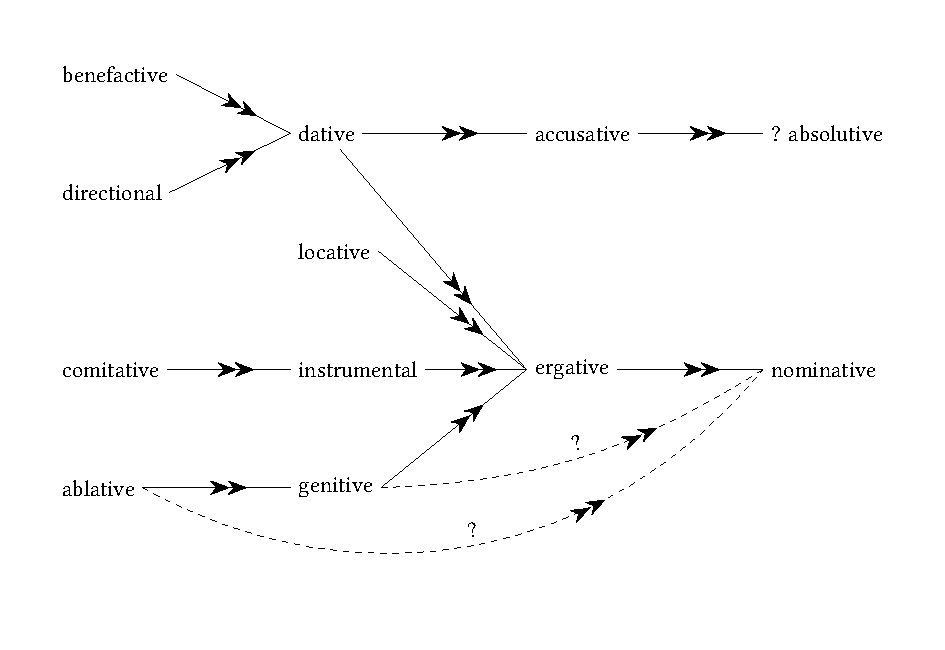
\includegraphics[width=.9\textwidth]{figures/8-someinterrelated.pdf}
\caption{Some interrelated grammaticalization channels of cases} \label{F8}
\end{figure}

\noindent\label{page120}More generally, \figref{F8} may be interpreted as a universal hierarchical layering to be found — presumably with modifications — in the case system of any individual language.\footnote{In the last two columns, the two rows represent, of course, alternative possibilities of systematic cooccurrence; we either have accusative and nominative, or ergative and absolutive.} The rightmost column constitutes the top of the hierarchy. Moving towards the left and thus descending the hierarchy, we do not arrive at any bottom. The adverbial relations discussed in \sectref{sec:3.4.1} may be arranged in similar rows and columns as above and may continue the scale to the left until grammar ceases and the lexicon begins.\footnote{This fact constitutes another principal challenge to the theory of case grammar; cf. \citet[76f]{Dillon1977}.} This layering, introduced already on p.~\pageref{page102}\chk%84
, may be captured by a number of specific hypotheses which use the criteria generally differentiating among degrees of grammaticality (see \sectref{chap:4}) and which together may be regarded as rendering the traditional notion of concrete vs. grammatical case more precise. One of these hypotheses, which takes up the considerations of p.~\pageref{page102}\chk%84
 , will be formulated here (see \citealt[§~4]{Lehmann1983}): There is a scale of structural means for the expression of case functions which starts with relational nouns and coverbs and passes through adverbs, adpositions and case markers to morphological zero expression. In every language, this scale is coupled with scale \figref{F8}, such that the least grammaticalized case functions are expressed by relational nouns or coverbs and the more grammaticalized ones successively by the other means. Both case functions and means may be skipped, but the order must be observed. Thus, the hypothesis means that each kind of structural means must be employed for a continuous segment of \figref{F8}. One more specific hypothesis entailed by this general one is: if a language has no segmental expression for some of the case functions, these form a continuous segment of \figref{F8}, starting from the right (top). With some minor exceptions, this is empirically true in an overwhelming number of languages.

 
%%please move the includegraphics inside the {figure} environment
%%\includegraphics[width=\textwidth]{\textsc{thoughts}-img5.svm}
\subsubsection{From functional sentence perspective to syntax} \label{sec:3.4.2.3}
The title of this section is reminiscent of Givón's “From discourse to syntax” (\citeyear{Givón1979}). In it, I shall report on the arguments presented in the literature (\citealt{LiEtAl1976}, \citealt{Sankoff1977}, \citealt{Hagège1978}, \citealt{Givón1979}, \citealt{Vincent1980a}) for the grammaticalization of communicative functions to syntactic functions.

The most common way to express a \textsc{topic} is by left-dislocating an \np and adjoining it as a coconstituent to a clause in which it is anaphorically resumed. This construction is becoming increasingly frequent in substandard French; see \citet{Ashby1981}. An example is \REF{ex:E92}.

\ea\label{ex:E92}
\langinfo{\LangFren}{}{}\\
 Jean, je l'ai vu hier.
\glt ‘John, I saw him yesterday.’\\
\z
\noindent There is no syntactic relation between the left-dislocated \np and the following clause or anything in it. One may therefore say that we are here at a level where syntax does not yet govern, where the discourse is structured only by the rules of functional sentence perspective.

Some languages have more or less circumlocutory means for marking the topic by more than mere sequential ordering. In German, we say \textit{was} \np \textit{betrifft/angeht} ‘as regards \np’, and in Portuguese and French, somewhat less clumsily, \textit{quanto a} = \textit{quant à} ‘as for’. The first step in the grammaticalization of such a construction is realized in Japanese. There is a postnominal particle \textit{wa}, which indicates that the preceding \np is the topic or the theme of the sentence. It may follow a bare \np, as in \REF{ex:E93}.a, or one equipped with a case marker, as in b.
 
\ea\label{ex:E93}
\langinfo{\LangJap}{}{} \\
 \ea \langinfo {\citep[43]{Jorden1962}}{}{}\\
 \gll {Matti}  {wa}  arimasen\\
  {match}  {\textsc{top}}  \textsc{exist}:\textsc{pol}:\textsc{neg}\\
\glt {‘As for matches, there aren't any.’ (topic), or:}\\
\glt {‘There aren't any matches.’ (theme)}\\
\ex \langinfo{\citep[101]{Jorden1962}}{}{}\\
\gll  Kyooto  e  wa  ikimasen  desita.\\
  Kyoto   \textsc{dir}   \textsc{top}   go:\textsc{pol}:\textsc{neg}   \textsc{aux}:\textsc{past}\\
\glt {‘To Kyoto, I did not go.’}\\
\z
\z
\noindent The theme is communicatively less salient than the topic; it is not set off by stress or a following pause, and syntactically, it is a constituent of its clause. Correspondingly, \textit{wa} is more grammatical than the topic locutions mentioned above. It is, in fact, in one distribution class, and thus mutually exclusive, with the subject marker \textit{ga} and the object marker \textit{o} (on which see below). Thus, while other \nps may keep their case markers, subject and object are neutralized before \textit{wa}.

Suppose now the following two things happen: First, for every verb, one of its semantically defined actants is destined to be the theme of a grammatically unmarked sentence. This would naturally not be done with arbitrary variation from verb to verb, but with a certain degree of semantic consistence. In particular, the agent will be a preferred theme. Second, the theme is generalized so that every sentence has one. How exactly these two steps are accomplished is largely a mystery; the empirical, in particular historical evidence for them is just not overwhelming. Anyway, both of them imply that the theme is deprived of its communicative function, because it can no longer vary independently of the syntax. It has been syntacticized, i.e. become a syntactic function. Every clause is conceived of as containing a predication about an \np which has this function, namely that of the \textsc{subject}. We thus get a grammaticalization channel ‘topic {\textgreater} theme {\textgreater} subject’ (cf. \citealt[484]{LiEtAl1976}, \citealt[83--85]{Givón1979}, \citealt[114]{Comrie1981b} and \citealt[99--101]{MallinsonEtAl1981}).

A by-product of this development is the subject-verb agreement (cf. p.~\pageref{page44}\chk%36
f.). As the left-dislocated \np is gradually integrated into the clause, the anaphoric pronoun referring to it is ousted from the subject position and becomes clitic to the verb. Since its referent is ultimately in the same clause, its function ceases to be anaphora and becomes agreement. Another form of the same development leads to the formation of a copula out of an anaphoric demonstrative, as we saw in \sectref{sec:3.1.2}.

A somewhat less common way of marking the topic is by right-dislocation. The resulting mode of expression, which is commonly called afterthought-\linebreak construction, occurs with some frequency in French (cf. \citealt[402, 427]{MallinsonEtAl1981}). An alternative to \REF{ex:E92} is \REF{ex:E94}.

\ea \label{ex:E94}
  Je l'ai vu hier, Jean
  \z
\noindent In French, neither left- nor right-dislocation will create new syntactic functions, because the subject and the object are already there. They do, however, lead to the grammaticalization of the anaphoric or cataphoric personal pronouns in the direction of agreement affixes, as the examples suggest. In other languages (see \citealt[119--121]{Hyman1975} and \citealt[170]{Vincent1980a}), the afterthought construction may be the only way of getting a nominal constituent after the verb of the clause. Therefore, if it is grammaticalized, the order of the main constituents may change. In particular, verb-initial basic word order may be assumed to arise in this way. If the subject and object are not universal, but are in complementary distribution with other organizations of the fundamental syntactic relations such as the ergative and absolutive, then these syntactic functions may not only be renovated by changes such as those exemplified or hypothesized above, but may also be created in the first place. The study of the change of accusative to ergative systems or vice versa should be able to provide the necessary empirical elucidations here.

The topicalization of the verb is a further instance of a construction which requires some circumlocution in languages such as German. The construction may be exemplified by \REF{ex:E95}.

\ea \label{ex:E95}
\langinfo{\LangGerm}\\
 Kochen tut sie nicht schlecht\\
\glt ‘As for cooking, she is not bad’
\z
\noindent In this analytic construction, the verb is split up into its lexical substance, represented by an infinitive, and its inflectional categories, represented by a finite form of the verb \textit{tun} ‘do’. The former is preposed, the latter takes the place of the main verb in the sentence. This is the regular verb topicalization construction in Standard German, to which there is no simpler alternative. The periphrastic expression is entirely motivated by the discourse function to be accomplished.\label{page123} However, in Substandard German this motivation may be absent, and we may have \textit{Sie tut nicht schlecht kochen} instead of the simple \textit{Sie kocht nicht schlecht} (cf. \citealt[156]{Ronneberger-Sibold1980} and p.~\pageref{page35}\chk%29
  above).

A last example of a construction which starts out at the discourse level with a given functional sentence perspective and then is syntacticized is the Indo-European relative construction which uses the *\textit{k}\textit{\textsuperscript{w}}\textit{i-/k}\textit{\textsuperscript{w}}\textit{o-} pronoun (cf. \citealt[Ch. \textsc{vi}.1]{Lehmann1984}). At the origin of the construction, there is a sequence of two independent sentences which are connected by functional sentence perspective: the first is the topic, the second the comment. One nominal in the first clause is marked by the *\textit{k}\textit{\textsuperscript{w}}\textit{i-/k}\textit{\textsuperscript{w}}\textit{o-} pronoun, which is originally an indefinite pronoun. The complex term which is thus implicitly formed by the first clause  is resumed in the next clause by an anaphoric pronoun. A passage such as ‘From the tree there will be shoots growing out from the ground; those you should press down into the ground’ would be expressed in this way. Its Latin manifestation would look like \REF{ex:E96}.a.

\ea\label{ex:E96}
\langinfo{Latin}{}{} \\
 \ea  \langinfo{(Cat. \textit{agr.} 51)}{}{}\\ 
 {\itshape Ab arbore abs terra pulli qui nascentur, eos in terram deprimito.}\\
 \glt ‘The shoots that will grow from the tree from the ground, those you should press down into the ground.’\\
\ex
   In terram deprimito pullos qui ... nascentur.\\
\glt  ‘You should press down into the ground the shoots that will grow ...’\\
\z
\z
\noindent \label{page125b}However, at the Latin stage the sequence is already slightly syntacticized into a complex sentence. \REF{ex:E96}.a shows the so-called correlative diptych. The relative clause is adjoined to the main clause, which means it is not its constituent and it has to either precede or follow it. At the origin, the relative clause always precedes the main clause. Later, the variant b and embedding of the relative clause become possible. Here the erstwhile indefinite pronoun has become a relative pronoun, the anaphoric pronoun vanishes, and the functional sentence perspective is no longer bound up with the construction. The relative construction is fully syntacticized.

Turning now to \textsc{focus} constructions, the most explicit way of marking the focus is the cleft-sentence. Its syntactic construction in the most diverse languages corresponds closely to the English pattern ‘it is \np that S’. To the extent that this is an autonomous pattern\footnote{The various attempts plainly to derive the cleft-sentence from a relative sentence must be considered failures; see \citealt[Ch.~V.5.3]{Lehmann1984}.}, the communicative function of focus is already minimally grammaticalized. Further grammaticalization will again reduce the syntactic complexity of the construction, simplifying the morphological means to an unanalyzable focus marker, e.g. Quechua -\textit{mi} \citep[35f]{Cole1982} and Somali \textit{baa} \citep[348f]{Sasse1977b}, and integrating the focus \np into the clause as a constituent with a regular syntactic function.

Focus constructions are grammaticalized as the normal expression of a word question in many languages. The question word is a grammaticalized focus.\footnote{\label{page125}This is the message of \citealt{Sasse1977b}, where the focus is mistakenly called topic. My discussion has also benefited from correspondence with H.-J. Sasse.} Accordingly, word questions may be constructed as cleft-sentences, for instance in French and Portuguese.

\ea\label{ex:E97}
\langinfo{\LangFren}{}{}\\
 \itshape Qu'est-ce qu'il fait?\\
 \glt ‘What is he doing?’\\
\z
\noindent \ea\label{ex:E98}
\langinfo{\LangPort}{}{}\\
\gll    Quando  é  que  ele  vem?\\
 when  is  that  he  comes\\
\glt {‘When will he come?’}\\
\z
\noindent Similarly, focus or rhematic particles will accompany question words:

\ea\label{ex:E99}
\langinfo{Quechua}{}{~\citep[18]{Cole1982}}\\
\gll may-pi-mi  pundaniki  inga-ka  kawsa-rka?\\
 where-\textsc{loc}-\textsc{foc}  first  Inka-\textsc{top}  live-\textsc{past}.3\\
\glt {‘Where did the first Inka live?’}\\
\z
\noindent \ea\label{ex:E100}
\langinfo{\LangSom}{}{~\citep[348]{Sasse1977b}}\\
 \ea
 \gll las  'aanood  b-uu  tegey.\\
   Las  Anod  \textsc{foc}-he  went\\
\glt {‘He went to Las Anod.’}\\
\ex
\gll  ħagg-uu  tegey?\\
  where:\textsc{foc}-he  went\\
\glt {‘Where did he go?’\footnotemark{}}\\
\z
\z
\footnotetext{\textit{buu} = \textit{baa}+\textit{uu}, \textit{ħagguu} = \textit{ħagge}+\textit{baa}+\textit{uu}.}

\noindent Further grammaticalization of this word question construction deletes the focus marker, leaving only the initial position of the question word, which is the unmarked order in numerous languages, including English and German. This is another example of the syntacticization of what was initially motivated by functional sentence perspective.

Another way of grammaticalizing focus markers is to associate them with definite syntactic functions. In Japanese, this concerns the subject and the direct object, while in Burmese it concerns these two and, in addition, the indirect object. If there is no emphasis on these constituents, they are left without case mark. If, however, they are in focus or otherwise stressed, postnominal case particles are attached to them, as shown in the following examples:

\ea\label{ex:E101}
\langinfo{Burmese}{}{} \\
 \ea \langinfo{\citep[4]{Kölver1985}}{}{}\\
 \gll  qamei  pawa  hya-ba-de.\\
  mother  handkerchief  search-\textsc{pol}-\textsc{fin}\\
\glt {‘Mother is looking for a handkerchief.’}\\
\ex
\gll  qamei-ga.  pawa  hya-ba-de.\\
 mother-\textsc{sbj}.\textsc{foc}  handkerchief search-\textsc{pol}-\textsc{fin}\\
\glt {‘It's mother who is looking for a handkerchief.’}\\
\ex \langinfo{\citep[9]{Kölver1985}}{}{}\\
\gll qamei pawa-gou hya-ba-de.\\
mother handkerchief-\textsc{obj}:\textsc{foc}  search-\textsc{pol}-\textsc{fin}\\
\glt {‘It's a handkerchief that mother is looking for.’}\\
\z
\z
\noindent \ea\label{ex:E102}
\langinfo{\LangJap}{}{}  \\
 \ea \langinfo{= \REF{ex:E93}.a}{}{}\\
 \gll  Matti  (wa)  arimasen\\
 match  \textsc{top}  \textsc{exist}:\textsc{pol}:\textsc{neg}\\
\glt {‘There áren't any matches.’}\\
\ex \langinfo{\citep[43]{Jorden1962}}{}{}\\
\gll  Matti  ga  arimasen.\\
 match  \textsc{sbj}.\textsc{foc} \textsc{exist}:\textsc{pol}:\textsc{neg}\\
\glt {‘There aren't any mátches.’ or: ‘It's matches what is lacking.’}\\
\z
\z
\noindent \ea\label{ex:E103}
\langinfo{\LangJap}{}{~\citep[44]{Jorden1962}}\\
 \ea
 \gll  Tabako  (wa)  kaimasita\\
   cigarette  \textsc{top}  buy:\textsc{pol}:\textsc{past}\\
\glt {‘Cigarettes I bought.’}\\
\ex
\gll  Tabako  o  kaimasita.\\
  cigarette  \textsc{obj}.\textsc{foc}  buy:\textsc{pol}:\textsc{past}\\
\glt {‘I bought cigarettes.’ or: ‘It's cigarettes what I bought.’}\\
\z
\z
\noindent As mentioned above, Burmese -\textit{ka.} has the ``Grundbedeutung'' of an ablative marker, and -\textit{kou} that of a directional. Japanese \textit{ga} goes back to a genitive marker, and \textit{o} to a perlative postposition. Thus, from the point of view of their meaning, these morphemes are relatively little grammaticalized for the syntactic functions which they mark in these examples. It seems therefore natural that they should be optional and only used for emphasis. It may be anticipated with some confidence that further grammaticalization will reduce these particles to plain case markers. The process has already begun in Japanese; the b-sentences may also be used without emphasis.

Despite the scarcity of relevant historical evidence, the development from discourse to syntax has attracted the attention of, and has seemed plausible to, several recent writers, including myself. I should like to quote some passages in order to give an impression of the importance that is being attributed to this matter. \citet[22]{Hagège1978} feels that

\begin{quote} \label{Hagege}
on peut considérer les contraintes syntaxiques comme le résultat du figement, avec démotivation plus ou moins importante, d'opérations qui, de sémantiquement et logiquement interprétables qu'elles ont été, ont pris le caractère mécanique de l'obligation qui définit ce qu'on appelle ”la grammaire“.
\end{quote}

\noindent Similarly, \citet[62]{Sankoff1977} states

\begin{quote}
that we can describe as syntacticization processes the transition between what initially appear to be ad hoc speaker strategies and what later can be fairly confidently described as syntactic rules.
\end{quote}

\noindent This may be summarized by \citet[107]{Givón1979} generalization that “human languages keep renovating their syntax via the grammaticalization of discourse.”

In what has been said above, it is implied that topic and focus, as they appear in left-dislocation and clefting, are completely free and wild, as it were, since they transcend the bounds of the simple sentence; whilst theme and rheme may be considered as tamed forms of the topic and the focus, respectively, since they may structure the simple sentence.\footnote{The theme-rheme structure of the simple sentence is grammaticalized in Imbabura Quechua \citep[95-98]{Cole1982}, which marks the theme by a suffix \textit{{}-ka} and the rheme by a suffix \textit{{}-mi}.} In a parallel fashion, the intonation contour is narrowed down on the way from topic/focus to theme/rheme: the pause after the topic, and the contrastive stress on the focus, are reduced. This is, of course, not compatible with everything that has been said about these concepts in the rather heterogeneous literature. However, as far as intonation is concerned, D. \citet{Bolinger1978} has expressed a similar view. Among the communicative (“attitudinal”) functions of the accent, he has the climatic, which tends to be associated with rightshift, and the emotional, which tends to be associated with backshift. Assuming that by ‘topic and comment’ he means what is here called theme and rheme, we may understand his suggestion (\citeyear[489]{Bolinger1978}): “The intonational treatment of topic and comment ... is probably a diluted and grammaticalized form of both the emotional and the climatic.” Such considerations are essential to the approach taken in this work, because they suggest that functional sentence perspective is not a homogeneous domain that could neatly be demarcated from semantics and syntax, but that, on the contrary, some parts of it are closer to free text formation and others are closer to syntax. I propose, then, somewhat reservedly, the grammaticalization scale of \figref{F9} (cf. \figref{fig:phases}).

The association of all the first elements and all the second elements of the pairs in the second row of \figref{F9} with each other seems possible, but not compulsory; speaking against this, we have seen subject markers expressing focus. The dots indicate that this is only the initial part of a grammaticalization scale and that it can probably be prolonged. A somewhat speculative guess would be ‘head/attribute’ as the next stage, still within syntax (cf. \citealt[Ch.~\textsc{iv}.2]{Lehmann1984}), although this construction also has different grammaticalizational origins, as we saw in \sectref{sec:3.3.3}.

\begin{figure}
\begin{tabular}{llll}

\multicolumn{2}{l}{functional sentence perspective} & syntax & morphology\\
\midrule
{topic/focus} & theme/rheme & subject/predicate & . . .\\

\end{tabular}
\caption{From discourse functions to syntactic functions}\label{F9}
\end{figure}


\noindent All of this was already anticipated by the father of grammaticalization, A. \citet[147f]{Meillet1912}. He compares free word order in Latin, which signals “expressive nuances”, with rigid word order in French, which expresses syntactic relations. For instance, subject and object of the predicate or the attribute of a head in Latin are identified independently of their sequential position and are distributed in the sentence according to its functional sentence perspective, whereas the same syntactic functions in French are identified exactly by the position of the constituents. This shows — says Meillet — that word order may be grammaticalized. Two comments may be appended to this. First, as we shall see in \sectref{sec:4.4}, reduction of word order freedom should be considered as one factor in a grammaticalization process which comprises more than that, namely the regulation of functional sentence perspective in terms of syntax, which then continues into morphology and further as indicated in \figref{fig:phases}. Second, Meillet's few remarks would seem to open up a particularly rich field of reliable historical evidence for the sort of development more postulated than demonstrated in this section.

\section{Conclusion}

In this survey of grammaticalization phenomena, the degree of detail has been rather uneven, some sections being comparatively thorough, others rather superficial. What is more, several parts of the grammar have not been mentioned at all. We have seen only some subordinating and no coordinating conjunctions, no sentence-type or other particles, no comparative and only a few possessive constructions, and so on. The material presented, however, should suffice to make my initial claim plausible, namely that grammaticalization is not a process restricted to some particular part of the grammatical system, but that it asserts itself everywhere between discourse structure and morphonology.

While we may safely assume this to be true, it is a different question whether it is possible for every grammatical category to be formed exclusively by grammaticalization. We have seen some examples of the grammaticalization of a periphrastic expression to a simple grammatical formative, where the periphrastic construction was formed not only by lexemes on their way towards grammaticalization, but also with the help of a grammatical formative of just the same category which would emerge as the result of the grammaticalization process. That is, while the grammatical formative of the output did continue a lexeme of the input, the input construction apparently presupposed the grammatical category which the output belonged to. Since reasonable discussion of this problem requires some theoretical background to be laid in the following chapters, we will defer it to §~8.3.
